\documentclass[10pt,letterpaper,final,twoside,notitlepage]{article}
\usepackage[margin=.5in]{geometry} % 1/2 inch margins on all pages
\usepackage[utf8]{inputenc} % Define the input encoding
\usepackage[USenglish]{babel} % Define language used
\usepackage{amsmath,amsfonts,amssymb}
\usepackage{amsthm} % Gives us plain, definition, and remark to use in \theoremstyle{style}
\usepackage{mathtools} % Allow for text and math in align* environment.
\usepackage{thmtools}
\usepackage{thm-restate}
\usepackage{graphicx}

\usepackage[
backend=biber,
style=alphabetic,
citestyle=authoryear]{biblatex} % Must include citation somewhere in document to print bibliography
\usepackage{hyperref} % Generate hyperlinks to referenced items
\usepackage[nottoc]{tocbibind} % Prints the Reference/Bibliography in TOC as well
\usepackage[noabbrev,nameinlink]{cleveref} % Fancy cross-references in the document everywhere
\usepackage{nameref} % Can make references by name to places
\usepackage{caption} % Allows for greater control over captions in figure, algorithm, table, etc. environments
\usepackage{subcaption} % Allows for multiple figures in one Figure environment
\usepackage[binary-units=true]{siunitx} % Gives us ways to typeset units for stuff
\usepackage{csquotes} % Context-sensitive quotation facilities
\usepackage{enumitem} % Provides [noitemsep, nolistsep] for more compact lists
\usepackage{chngcntr} % Allows us to tamper with the counter a little more
\usepackage{empheq} % Allow boxing of equations in special math environments
\usepackage[x11names]{xcolor} % Gives access to coloring text in environments or just text, MUST be before tikz
\usepackage{tcolorbox} % Allows us to create boxes of various types for examples
\usepackage{tikz} % Allows us to create TikZ and PGF Pictures
\usepackage{ctable} % Greater control over tables and how they look
\usepackage{diagbox} % Allow us to have shared diagonal cells in tables
\usepackage{multirow} % Allow us to have a single cell in a table span multiple rows
\usepackage{titling} % Put document information throughout the document programmatically
\usepackage[linesnumbered,ruled,vlined]{algorithm2e} % Allows us to write algorithms in a nice style.

\counterwithin{figure}{section}
\counterwithin{table}{section}
\counterwithin{equation}{section}
\counterwithin{algocf}{section}
\crefname{algocf}{algorithm}{algorithms}
\Crefname{algocf}{Algorithm}{Algorithms}
\setcounter{secnumdepth}{4}
\setcounter{tocdepth}{4} % Include \paragraph in toc
\crefname{paragraph}{paragraph}{paragraphs}
\Crefname{paragraph}{Paragraph}{Paragraphs}

% Create a theorem environment
\theoremstyle{plain}
\newtheorem{theorem}{Theorem}[section]
% Create a numbered theorem-like environment for lemmas
\newtheorem{lemma}{Lemma}[theorem]

% Create a definition environment
\theoremstyle{definition}
\newtheorem{definition}{Defn}
\newtheorem{corollary}{Corollary}[section]
% \begin{definition}[Term] \label{def:}
%   Make sure the term is emphasized with \emph{term}.
%   This ensures that if \emph is changed, it shows up everywhere
% \end{definition}

% Create a numbered remark environment numbered based on definition
% NOTE: This version of remark MUST go inside a definition environment
\theoremstyle{remark}
\newtheorem{remark}{Remark}[definition]
%\counterwithin{definition}{subsection} % Uncomment to have definitions use section.subsection numbering

% Create an unnumbered remark environment for general use
% NOTE: This version of remark has NO restrictions on placement
\newtheorem*{remark*}{Remark}

% Create a special list that handles properties. It can be broken and restarted
\newlist{propertylist}{enumerate}{1} % {Name}{Template}{Max Depth}
% [newlistname, LevelsToApplyTo]{formatting options}
\setlist[propertylist, 1]{label=\textbf{(\roman*)}, ref=\textbf{(\roman*)}, noitemsep, nolistsep}
\crefname{propertylisti}{property}{properties}
\Crefname{propertylisti}{Property}{Properties}

% Create a special list that handles enumerate starting with lower letters. Breakable/Restartable.
\newlist{boldalphlist}{enumerate}{1} % {Name}{Template}{Max Depth}
% [newlistname, LevelsToApplyTo]{formatting options}
\setlist[boldalphlist, 1]{label=\textbf{(\alph*)}, ref=\alph*, noitemsep, nolistsep} % Set options

\newlist{nocrefenumerate}{enumerate}{1} % {Name}{Template}{Max Depth}
% [newlistname, LevelsToApplyTo]{formatting options}
\setlist[nocrefenumerate, 1]{label=(\arabic*), ref=(\arabic*), noitemsep, nolistsep}

% Create a list that allows for deeper nesting of numbers. By default enumerate only allows depth=4.
\newlist{nestednums}{enumerate}{6}
% [newlistname, LevelsToApplyTo]{formatting options}
\setlist[nestednums]{noitemsep, label*=\arabic*.}

\tcbuselibrary{breakable} % Allow tcolorboxes to be broken across pages
% Create a tcolorbox for examples
% /begin{example}[extra name]{NAME}
% Create a tcolorbox for examples
% Argument #1 is optional, given by [], that is the textbook's problem number
% Argument #2 is mandatory, given by {}, that is the title for the example
% Avoid putting special characters, (), [], {}, ",", etc. in the title.
\newtcolorbox[auto counter,
number within=section,
number format=\arabic,
crefname={example}{examples}, % Define reference format for cref (No Capitals)
Crefname={Example}{Examples}, % Reference format for cleveref (With Capitals)
]{example}[2][]{ % The [2][] Means the first argument is optional
  width=\textwidth,
  title={Example \thetcbcounter: #2. #1}, % Parentheses and commas are not well supported
  fonttitle=\bfseries,
  label={ex:#2},
  nameref=#2,
  colbacktitle=white!100!black,
  coltitle=black!100!white,
  colback=white!100!black,
  upperbox=visible,
  lowerbox=visible,
  sharp corners=all,
  breakable
}

% Create a tcolorbox for general use
\newtcolorbox[% auto counter,
% number within=section,
% number format=\arabic,
% crefname={example}{examples}, % Define reference format for cref (No Capitals)
% Crefname={Example}{Examples}, % Reference format for cleveref (With Capitals)
]{blackbox}{
  width=\textwidth,
  % title={},
  fonttitle=\bfseries,
  % label={},
  % nameref=,
  colbacktitle=white!100!black,
  coltitle=black!100!white,
  colback=white!100!black,
  upperbox=visible,
  lowerbox=visible,
  sharp corners=all
}

% Redefine the 'end of proof' symbol to be a black square, not blank
\renewcommand{\qedsymbol}{$\blacksquare$} % Change proofs to have black square at end

% Common Mathematical Stuff
\newcommand{\Abs}[1]{\ensuremath{\lvert #1 \rvert}}
\newcommand{\DNE}{\ensuremath{\mathrm{DNE}}} % Used when limit of function Does Not Exist

% Complex Numbers functions
\renewcommand{\Re}{\operatorname{Re}} % Redefine to use the command, but not the fraktur version
\renewcommand{\Im}{\operatorname{Im}} % Redefine to use the command, but not the fraktur version
\newcommand{\Real}[1]{\ensuremath{\Re \lbrace #1 \rbrace}}
\newcommand{\Imag}[1]{\ensuremath{\Im \lbrace #1 \rbrace}}
\newcommand{\Conjugate}[1]{\ensuremath{\overline{#1}}}
\newcommand{\Modulus}[1]{\ensuremath{\lvert #1 \rvert}}
\DeclareMathOperator{\PrincipalArg}{\ensuremath{Arg}}

% Math Operators that are useful to abstract the written math away to one spot
% Number Sets
\DeclareMathOperator{\RealNumbers}{\ensuremath{\mathbb{R}}}
\DeclareMathOperator{\AllIntegers}{\ensuremath{\mathbb{Z}}}
\DeclareMathOperator{\PositiveInts}{\ensuremath{\mathbb{Z}^{+}}}
\DeclareMathOperator{\NegativeInts}{\ensuremath{\mathbb{Z}^{-}}}
\DeclareMathOperator{\NaturalNumbers}{\ensuremath{\mathbb{N}}}
\DeclareMathOperator{\ComplexNumbers}{\ensuremath{\mathbb{C}}}
\DeclareMathOperator{\RationalNumbers}{\ensuremath{\mathbb{Q}}}

% Calculus operators
\DeclareMathOperator*{\argmax}{argmax} % Thin Space and subscripts are UNDER in display

% Signal and System Functions
\DeclareMathOperator{\UnitStep}{\mathcal{U}}
\DeclareMathOperator{\sinc}{sinc} % sinc(x) = (sin(pi x)/(pi x))

% Transformations
\DeclareMathOperator{\Lapl}{\mathcal{L}} % Declare a Laplace symbol to be used

% Logical Operators
\DeclareMathOperator{\XOR}{\oplus}

% x86 CPU Registers
\newcommand{\rbpRegister}{\texttt{\%rbp}}
\newcommand{\rspRegister}{\texttt{\%rsp}}
\newcommand{\ripRegister}{\texttt{\%rip}}
\newcommand{\raxRegister}{\texttt{\%rax}}
\newcommand{\rbxRegister}{\texttt{\%rbx}}

%%% Local Variables:
%%% mode: latex
%%% TeX-master: shared
%%% End:


% These packages are more specific to certain documents, but will be availabe in the template
% \usepackage{esint} % Provides us with more types of integral symbols to use
% \usepackage[outputdir=./TeX_Output]{minted} % Allow us to nicely typeset 300+ programming languages
% This document must be compiled with the -shell-escape flag if the packages above are uncommented
\usepackage{polynom} % Give access to commands to perform long division automatically

\graphicspath{{./Drawings/EDIN01-Cryptography}} % Uncomment this to use pictures in this document
% \addbibresource{./Bibliographies/EDIN01-Cryptography.bib}

% Math Operators that are useful to abstract the written math away to one spot
% These are supposed to be document-specific mathematical operators that will make life easier
% Many fundamental operators are defined in Reference_Sheet_Preamble.tex

\DeclareMathOperator{\Divides}{\vert}
\DeclareMathOperator{\DIV}{\operatorname{div}}
\DeclareMathOperator{\lcm}{\operatorname{lcm}}
\DeclareMathOperator{\ElementOrder}{\operatorname{ord}}
\newcommand{\SetOrder}[1]{\lvert #1 \rvert}
\newcommand{\TextSetOrder}[1]{$\SetOrder{#1}$}
\newcommand{\BinaryOperation}{*}
\DeclareMathOperator{\Degree}{\operatorname{deg}}

% REQUIRES THAN \AllIntegers BE DEFINED BEFORE MAKING THE NEW COMMAND
% \input-ing the Reference Preamble before here handles this for you.
% \IntsMod{#} takes something and subscripts it with the all integers symbol
% These commands MUST be placed inside of a math environment to work
\newcommand{\IntsMod}[1]{\AllIntegers_{#1}}
% Wrapper command. You don't need to specify anything because n is specified as the modulus for you
\newcommand{\IntsModN}{\IntsMod{n}}
\newcommand{\TextIntsMod}[1]{$\IntsMod{#1}$}
% Wrapper command. You don't need to specify anything because n is specified as the modulus for you
\newcommand{\TextIntsModN}{$\IntsModN{}$}
\newcommand{\MultiplicativeGroup}[1]{\IntsMod{#1}^{*}}
\newcommand{\MultiplicativeGroupN}{\IntsModN^{*}}
\newcommand{\TextMultiplicativeGroup}[1]{$\IntsMod{#1}^{*}$}
\newcommand{\TextMultiplicativeGroupN}{$\IntsModN^{*}$}

% Used to denote cyclic subgroups
\newcommand{\CyclicSubgroup}[1]{<#1>}
\newcommand{\TextCyclicSubgroup}[1]{$\CyclicSubgroup{#1}$}
\newcommand{\MathField}[2]{#1[#2]}
\newcommand{\TextMathField}[2]{$\MathField{#1}{#2}$}
\newcommand{\FiniteMathField}[3]{\mathbb{#1}_{#2^{#3}}}
\newcommand{\TextFiniteMathField}[3]{$\FiniteMathField{#1}{#2}{#3}$}

\newcommand{\PolynomialRing}[3]{\MathField{#1_{#2}}{#3}}
\newcommand{\TextPolynomialRing}[3]{$\PolynomialRing{#1}{#2}{#3}$}
\newcommand{\FinitePolynomialRing}[3]{\MathField{\mathbb{#1}_{#2}}{#3}}
\newcommand{\TextFinitePolynomialRing}[3]{$\PolynomialRing{#1}{#2}{#3}$}

\DeclareMathOperator{\Plaintexts}{\mathcal{P}}
\DeclareMathOperator{\Messages}{\mathcal{M}}
\DeclareMathOperator{\Alphabet}{\mathcal{A}}
\DeclareMathOperator{\Message}{\mathbf{m}}
\DeclareMathOperator{\Ciphertexts}{\mathcal{C}}
\DeclareMathOperator{\CipherMessage}{\mathbf{c}}
\DeclareMathOperator{\Keyspace}{\mathcal{K}}
\DeclareMathOperator{\EncryptionRules}{\mathcal{E}}
\DeclareMathOperator{\DecryptionRules}{\mathcal{D}}
\DeclareMathOperator{\SourceMessages}{\mathcal{S}} % Only used in Authentication Section
\DeclareMathOperator{\ChannelMessages}{\mathcal{M}} % Only used in Authentication Section
\DeclareMathOperator{\MessageTags}{\mathcal{Z}} % Only used in Authentication Section
\DeclareMathOperator{\Participants}{\mathcal{P}}
\DeclareMathOperator{\SomeParticipants}{\mathcal{B}}
\DeclareMathOperator{\MoreParticipants}{\mathcal{C}}
\DeclareMathOperator{\Shares}{\mathcal{S}}
\DeclareMathOperator{\AccessStructure}{\Gamma}
\DeclareMathOperator{\QualifiedSubset}{\Gamma}
\DeclareMathOperator{\Closure}{\text{cl}}

\DeclareMathOperator{\Prob}{\operatorname{P}}
\DeclareMathOperator{\ExpectedValue}{\operatorname{\mathbb{E}}}
\DeclareMathOperator{\Given}{\vert}
\DeclareMathOperator{\Entropy}{\operatorname{H}}
\DeclareMathOperator{\BinaryEntropy}{\operatorname{h}}
\DeclareMathOperator{\RelativeEntropy}{\operatorname{D}}
\DeclareMathOperator{\Between}{\Vert}
\DeclareMathOperator{\MutualInformation}{\operatorname{I}}

\begin{titlepage}
  \title{EDIN01: Cryptography --- Reference Sheet \\ Lund University}
  \author{Karl Hallsby}
  \date{Last Edited: \today} % We want to inform people when this document was last edited
\end{titlepage}

\begin{document}
\pagenumbering{gobble}
\maketitle
\pagenumbering{roman} % i, ii, iii on beginning pages, that don't have content
\tableofcontents
\clearpage
\listoftheorems[ignoreall, show={definition, Definition}]
\clearpage
\pagenumbering{arabic} % 1,2,3 on content pages

\section{Cryptography Introduction}\label{sec:Intro_Cryptography}
\begin{definition}[Cryptographic Primitive]\label{def:Cryptographic_Primitive}
  A \emph{cryptographic primitive} is an algorithm with basic cryptographic properties.
\end{definition}

\begin{definition}[Cryptographic Protocol]\label{def:Cryptographic_Protocol}
  A \emph{cryptographic protocol} involves the back-and-forth communication among two or more parties.

  \begin{remark}[Bob and Alice]\label{rmk:Bob_and_Alice}
    Typically, the parties are named Bob and Alice.
    These are arbitrary names, but these are the most commonly used ones.
  \end{remark}
\end{definition}

There are have been several \nameref{def:Cryptographic_Protocol}s.
\begin{enumerate}[noitemsep]
\item \textit{Symmetric-key cryptography} - Methods in which both the sender and receiver share the same key
  \begin{enumerate}[noitemsep]
  \item Block ciphers
  \item Stream ciphers
  \item MAC algorithms
  \end{enumerate}
\item \textit{Public-key cryptography}: 2 different, but mathematically related keys are used.
  A public key and a private key.
  \begin{enumerate}[noitemsep]
  \item The public key cannot decrypt something that was encrypted with the private key.
  \item The public key can be shared freely, because the private key cannot be generated from the public key.
  \end{enumerate}
\item \textit{Cryptographic hash functions} are a related and important class of cryptographic algorithms.
  \begin{enumerate}[noitemsep]
  \item This is a keyless \nameref{def:Cryptographic_Primitive}.
  \item Takes an arbitrary length input and produces a fixed-length output.
  \item The mapping between the input and output is such that the output cannot generate the input, therefore making it cryptographic.
  \end{enumerate}
\end{enumerate}

\subsection{Historical Cryptography}\label{subsec:Historical_Cryptography}
Just to give a super quick background on how we've gotten to where we are today when it comes to cryptography.

\subsubsection{Monoalphabetic Ciphers}\label{subsubsec:Monoalphabetic_Ciphers}
\begin{definition}[Monoalphabetic Cipher]\label{def:Monoalphabetic_Cipher}
  In a \emph{monoalphabetic cipher} a single letter is replaced by the cipher's mapping.
  Since the cipher can do this to arbitrary letters, this could continue indefinitely for any single letter.

  These were some of the first ciphers developed by Man.
  These include simple substitute ciphers, and letter shifting ciphers.
  However, these can be broken with \emph{frequency analysis}.
\end{definition}

\subsubsection{Polyalphabetic Ciphers}\label{subsubsec:Polyalphabetic_Ciphers}
\begin{definition}[Polyalphabetic Cipher]\label{def:Polyalphabetic_Cipher}
  In a \emph{polyalphabetic cipher} multiple letters are replaced by the cipher's mapping.
  Additionally, since the cipher can output multiple letters, the ciphered letters could be run through the cipher again.

  These were developed in response to \nameref{def:Monoalphabetic_Cipher}s being broken.
  However, these can also be broken, with \emph{extended frequency analysis}.
\end{definition}

Eventually, it was realized that the secrecy of the cipher is not sensible/possible.
This leads us to the conclusion that \textbf{any cryptographic scheme should remain secure even if the adversary understands the cipher algorithm itself}.

\subsubsection{Cryptographic Keys}\label{subsubsec:Cryptographic_Keys}
The use of keys as ciphers is a slightly more modern occurrence.
\begin{definition}[Kerckhoff's Principle]\label{def:Kerckhoffs_Principle}
  \emph{Kerckhoff's Principle} states that the security of the key used should alone be sufficient for a good cipher to maintain confidentiality under an attack.
  Essentially, the security of the key used should be sufficient such that the cipher can be maintained confidently while under attack.
\end{definition}

However, only since the mid-1970s, has public key cryptography has been possible.

\begin{table}[h!]
  \centering
  \begin{tabular}{cc}
    \toprule
    Symmetric-Key Cryptography & Public-Key Cryptography \\
    \midrule
    Block ciphers & Public-Key encryption \\
    Stream ciphers & Digital Signature Schemes \\
    Cryptographic Hash Functions & Key exchange protocols \\
                               & Electronic Cash/Cryptocurrency \\
                               & Interactive Proof Systems \\
    \bottomrule
  \end{tabular}
  \caption{Uses of Key-Based Cryptography}
  \label{tab:Key_Cryptography_Uses}
\end{table}

Computers can efficiently encrypt, given the following constraints:
\begin{enumerate}[noitemsep]
\item Some modern techniques can only keep the keys secret if certain mathematical problems are \nameref{def:Intractable}.
  \begin{enumerate}[noitemsep]
  \item Integer factorization
  \item Discrete logarithm problems
  \end{enumerate}
\item However, there are no absolute proofs that a cryptographic technique is secure.
\end{enumerate}

\begin{definition}[Intractable]\label{def:Intractable}
  An \emph{intractable} problem is one in which there are no \textbf{efficient} algorithms to solve them.
\end{definition}

%%% Local Variables:
%%% mode: latex
%%% TeX-master: "../EDIN01-Cryptography-Reference_Sheet"
%%% End:


\section{Number Theory}\label{sec:Number_Theory}
Before we can start with any of the deeper cryptography stuff, we need to start with some basic number theory.
\begin{definition}[Number Theory]\label{def:Number_Theory}
  \emph{Number theory} is a branch of pure mathematics devoted primarily to the study of the integers and integer-valued functions.
  Number theorists study prime numbers as well as the properties of objects made out of integers (for example, rational numbers) or defined as generalizations of the integers (for example, algebraic integers).
\end{definition}

\begin{definition}[Divides]\label{def:Divides}
  For $a, b \in \AllIntegers$, we say that $a$ \emph{divides} $b$ (written $a \divides b$) if there exists an integer $c$ such that $b = ac$.

  Properties:
  \begin{propertylist}
  \item $a \divides a$
  \item If $a \divides b$ and $b \divides c$, then $a \divides c$.
  \item If $a \divides b$ and $a \divides c$, then $a \divides (bx + cy)$ for any $x, y \in \AllIntegers$.
  \item If $a \divides b$ and $b \divides a$, then $a = \pm b$.
  \end{propertylist}
\end{definition}

\subsection{Quotient and Remainder}\label{subsec:Quotient_and_Remainder}
For $a, b \in \AllIntegers$, with $b \geq 1$.
Then an ordinary long division of $a$ by $b$, i.e. $a \div b$ yields two integers $q$ and $r$ such that
\begin{equation}\label{eq:Quotient_and_Remainder}
  a = qb + r, \text{where } 0 \leq r < b
\end{equation}

$q$ and $r$ are called the \nameref{def:Quotient} and \nameref{def:Remainder}, respectively, and are \textbf{unique}.

\begin{definition}[Quotient]\label{def:Quotient}
  The \emph{quotient}, $q$, of $a$ divided by $b$ is denoted $a \DIV b$.
\end{definition}

\begin{definition}[Remainder]\label{def:Remainder}
  The \emph{remainder}, $r$, of $a$ divided by $b$ is denoted $a \bmod b$.
\end{definition}

\begin{example}[]{Quotient and Remainder}
  If $a=53$ and $b=9$, what is $a \bmod b$?

  \tcblower{}

  \begin{align*}
    53 &= q9 + r \\
    q &= 5 \\
    r &= 8
  \end{align*}
\end{example}

\subsection{Greatest Common Divisor}\label{subsec:Greatest_Common_Divisor}
\begin{definition}[Common Divisor]\label{def:Common_Divisor}
  An integer $c$ is a \emph{common divisor} of $a$ and $b$ if $c \divides a$ and $c \divides b$.
\end{definition}

\begin{definition}[Greatest Common Divisor]\label{def:GCD}
  A non-negative integer $d$ is called the \emph{greatest common divisor} (\emph{GCD}) of integers $a$ and $b$ if:
  \begin{enumerate}[noitemsep]
  \item $d$ is a \nameref{def:Common_Divisor} of $a$ and $b$.
  \item For every other common divisor $c$ it holds that $c \divides d$.
  \end{enumerate}

  The greatest common divisor is denoted
  \begin{equation}\label{eq:GCD}
    \gcd(a, b)
  \end{equation}

  $\gcd(a,b)$ is the \textbf{largest positive} integer dividing both $a$ and $b$ (except for $\gcd(0,0)=0$).
  
  \begin{remark}
    If $a, b \in \PositiveInts$, then $\lcm(a, b) \cdot \gcd(a, b) = a \cdot b$
  \end{remark}
\end{definition}

\begin{example}[]{Greatest Common Divisor}
  What is the $\gcd(18, 24)$?

  \tcblower{}

  Common Divisors = $\lbrace \pm 1, \pm 2, \pm 4, \pm 6 \rbrace$.

  Since we can only allow positive integers,
  \begin{equation*}
    \gcd(18, 24) = +6
  \end{equation*}
\end{example}

\subsection{Least Common Multiple}\label{subsec:Least_Common_Multiple}
\begin{definition}[Least Common Multiple]\label{def:LCM}
  A non-negative integer $d$ is called the \emph{least common multiple} (\emph{LCM}) of integers $a$ and $b$ if:
  \begin{enumerate}[noitemsep]
  \item $a \divides d$ and $b \divides d$
  \item For every integer $c$ such that $a \divides c$ and $b \divides c$, we have $d \divides c$.
  \end{enumerate}

  The least common multiple is denoted
  \begin{equation}\label{eq:LCM}
    \lcm(a, b)
  \end{equation}

  $\lcm(a, b)$ is the \textbf{smallest positive} integer divisible by both $a$ and $b$.

  \begin{remark}
    If $a, b \in \PositiveInts$, then $\lcm(a, b) \cdot \gcd(a, b) = a \cdot b$
  \end{remark}
\end{definition}

\subsection{Primality}\label{subsec:Primality}
\begin{definition}[Relatively Prime]\label{def:Relatively_Prime}
  $a, b$ are called \emph{relatively prime} if $\gcd(a, b) = 1$.
\end{definition}

\begin{definition}[Prime]\label{def:Prime}
  An integer $p \geq 2$ is called \emph{prime} if its only positive divisors are $1$ and $p$.
  Otherwise, $p$ is called a \emph{\nameref{def:Composite}}.
\end{definition}

\begin{definition}[Composite]\label{def:Composite}
  An integer $p \geq 2$ is called \emph{composite} if it has more positive divisors than just $1$ and $p$.
  Otherwise, $p$ is called a \emph{\nameref{def:Prime}}.
\end{definition}

\subsubsection{Number of Primes}\label{subsubsec:Number_of_Primes}
The number of primes $\leq x$ is denoted
\begin{equation}\label{eq:Number_of_Primes}
  \pi(x)
\end{equation}
\begin{enumerate}[noitemsep]
\item There are infinitely many primes
\item $\lim\limits_{x \rightarrow \infty} \frac{\pi(x)}{\frac{x}{\ln(x)}} = 1$
\item For $x \geq 17$, $\frac{x}{\ln(x)} < \pi(x) < \frac{1.25506x}{\ln(x)}$
\end{enumerate}

\subsection{Unique Factorization}\label{subsec:Unique_Factorization}
\begin{theorem}[Unique Factorization Theorem]\label{thm:Unique_Factorization_Theorem}
  Every integer $n \geq 2$ can be written as a product of prime powers,
  \begin{equation*}
    n = p_{1}^{e_{1}} p_{2}^{e_{2}} \cdots p_{k}^{e_{k}}
  \end{equation*}
  where $p_{1}, p_{2}, \ldots p_{k}$ are distinct primes and $e_{1}, e_{2}, \ldots e_{k}$ are positive integers.
  Furthermore, the factorization is unique up to rearrangement of the factors.
\end{theorem}

\subsubsection{\nameref{def:GCD} and \nameref{def:LCM} with Unique Factors}\label{subsubsec:GCD_LCM_Unique_Factors}
If $a = p_{1}^{e_{1}} p_{2}^{e_{2}} \cdots p_{k}^{e_{k}}$ and $b = p_{1}^{f_{1}} p_{2}^{f_{2}} \cdots p_{k}^{e_{k}}$, where $e_{i}, f_{i}, i = 1, 2, \ldots k$ are non-negative integers, then
\begin{equation}\label{eq:GCD_Unique_Factors}
  \gcd(a, b) = p_{1}^{\min(e_{1}, f_{1})} p_{2}^{\min(e_{2}, f_{2})} \cdots p_{k}^{\min(e_{k}, f_{k})}
\end{equation}
and
\begin{equation}\label{eq:LCM_Unique_Factors}
  \lcm(a, b) = p_{1}^{\max(e_{1}, f_{1})} p_{2}^{\max(e_{2}, f_{2})} \cdots p_{k}^{\max(e_{k}, f_{k})}
\end{equation}

\subsection{Euler Phi Function}\label{subsec:Euler_Phi_Function}
\begin{definition}[Euler Phi Function]\label{def:Euler_Phi_Function}
  For $n \geq 1$, let $\phi(n)$ denote the number of integers in the interval $[1, n]$, which are \nameref{def:Relatively_Prime} to $n$.
  This function is called the \emph{Euler Phi Function}.
\end{definition}
\begin{theorem}[Euler Phi Function]\label{thm:Euler_Phi_Function}
  There are a few properties of the \nameref{def:Euler_Phi_Function} that we will treat as true because of this theorem.
  \begin{enumerate}[noitemsep]
  \item If $p$ is a \nameref{def:Prime}, then $\phi(p) = p - 1$.
  \item If $\gcd(a, b) = 1$, then $\phi(ab) = \phi(a) \phi(b)$.
  \item If $n = p_{1}^{e_{1}} p_{2}^{e_{2}} \cdots p_{k}^{e_{k}}$, then
    \begin{equation*}
      \phi(n) = \left( p_{1}^{e_{1}} - p_{1}^{e_{1}-1} \right) \left( p_{2}^{e_{2}} - p_{2}^{e_{2}-1} \right) \cdots \left( p_{k}^{e_{k}} - p_{k}^{e_{k}-1} \right)
    \end{equation*}
  \end{enumerate}
\end{theorem}

\begin{lemma}[Computing the \nameref{def:GCD}]\label{lemma:Compute_GCD}
  If $a$ and $b$ are positive integers where $a > b$, then
  \begin{equation}\label{eq:Compute_GCD}
    \gcd(a, b) = \gcd(b, a \bmod b)
  \end{equation}
  \begin{remark*}
    This can be repeated to efficiently calculate the $\gcd(a, b)$.
    This is called the \nameref{def:Euclidean_Algorithm}.
  \end{remark*}
\end{lemma}

\begin{definition}[Euclidean Algorithm]\label{def:Euclidean_Algorithm}
  The \emph{euclidean algorithm} is a way to efficiently calculate the $\gcd(a, b)$.
  \begin{enumerate}[noitemsep]
  \item Set $r_{0} \leftarrow a, r_{1} \leftarrow b, i \leftarrow 1$.
  \item While $r_{i} \neq 0$ do:
    \begin{enumerate}[noitemsep]
    \item Set $r_{i+1} \leftarrow r_{i-1} \bmod r_{i}, i \leftarrow i+1$
    \end{enumerate}
  \item Return $r_{i}$
  \end{enumerate}
\end{definition}

\begin{example}{Euclidean Algorithm}
  Find the \nameref{def:GCD} of 147 and 273?

  \tcblower{}

  \begin{align*}
    273 = 1 \cdot 147 + 126 &\Rightarrow \gcd(126, 147) \\
    147 = 1 \cdot 126 + 21 &\Rightarrow \gcd(21, 126) \\
    126 = 6 \cdot 21 + 0 &\Rightarrow \gcd(21, 126) \\
  \end{align*}

  Thus, since $6 \cdot 21 = 126$, 21 is the \nameref{def:GCD} of 147 and 273.
\end{example}

\begin{theorem}
  There exist integers $x, y$ such that $\gcd(a, b)$ can be written as
  \begin{equation}\label{eq:Extended_Euclidean_Algorithm_Basis}
    \gcd(a, b) = ax + by
  \end{equation}
\end{theorem}
\begin{proof}
  \begin{align*}
    \gcd(a, b) &= r_{i} \\
               &= r_{i-2} - q_{i-1}r_{i-1} \\
               &= r_{i-2} - q_{i-1}(r_{i-3} - q_{i-2}r_{i-2}) \\
               &\vdots \\
               &= r_{0}x + r_{1}y \\
               &= ax + by
  \end{align*}
  for some integers $x, y \in \AllIntegers$.
\end{proof}

This means that the \nameref{def:Euclidean_Algorithm} can be extended to return the values of $x$ and $y$ from \Cref{eq:Extended_Euclidean_Algorithm_Basis}.

\begin{definition}[Extended Euclidean Algorithm]\label{def:Extended_Euclidean_Algorithm}
  The \emph{extended euclidean algorithm} is a way to efficiently calculate the linear pair of integers ($x, y \in \AllIntegers$) that satisfy \Cref{eq:Extended_Euclidean_Algorithm_Basis}.
  \begin{equation*}
    \gcd(a, b) = ax + by
  \end{equation*}

  \begin{enumerate}[noitemsep]
  \item If $b = 0$, then return $a, x \leftarrow 1, y \leftarrow 0$.
  \item Set $x_{2} \leftarrow 1, x_{2} \leftarrow 0, y_{2} \leftarrow 0, y_{1} \leftarrow 1$
  \item While $b > 0$ do:
    \begin{enumerate}[noitemsep]
    \item $q \leftarrow a \DIV b, r \leftarrow a-qb, x \leftarrow x_{2} - qx_{1}, y \leftarrow y_{2} - qy_{1}$
    \item $a \leftarrow b, b \leftarrow r, x_{2} \leftarrow x_{1}, x_{1} \leftarrow x, y_{2} \leftarrow y_{1}, y_{1} \leftarrow y$.
    \end{enumerate}
  \item Set $d \leftarrow a, x \leftarrow x_{2}, y \leftarrow y_{2}$ and return $d, x, y$.
  \end{enumerate}
\end{definition}

\subsection{\texorpdfstring{The Integers modulo $n$}{The Integers modulo n}}\label{subsec:Integer_Modulo_n}
Let $n$ be a positive integer.
\begin{definition}[Congruence]\label{def:Congruence}
  If $a$ and $b$ are integers, then \emph{$a$ is said to be congruent to $b$ modulo $n$}, which is written as
  \begin{equation}\label{eq:A_Congruent_B}
    a \equiv b \pmod{n}
  \end{equation}

  If $n$ divides $(a-b)$, i.e. $n \divides (a-b)$, then we call $n$ the \emph{modulus} of the congruence.

\end{definition}

\begin{theorem}
  For $a, a_{1}, b, b_{1}, c\in \AllIntegers$, we have
  \begin{propertylist}
  \item $a \equiv b \pmod{n}$ \emph{if and only if} $a$ and $b$ leave the same \nameref{def:Remainder} when divided by $n$.
  \item $a \equiv a \pmod{n}$ \label{prop:A_Congruent_B_Reflexivity}
  \item If $a \equiv b \pmod{n}$, then $b \equiv a \pmod{n}$ \label{prop:A_Congruent_B_Symmetry}
  \item If $a \equiv b \pmod{n}$ adn $b \equiv c \pmod{n}$, then $a \equiv c \pmod{n}$ \label{prop:A_Congruent_B_Transitivity}
  \item If $a \equiv a_{1} \pmod{n}$ and $b \equiv b_{1} \pmod{n}$, then $a+b = a_{1} + b_{1} \pmod{n}$ and $ab = a_{1}b_{1} \pmod{n}$.
  \end{propertylist}

  The \crefrange{prop:A_Congruent_B_Reflexivity}{prop:A_Congruent_B_Transitivity} are called \emph{reflexivity}, \emph{symmetry}, and \emph{transitivity}, respectively.
\end{theorem}

\subsection{Equivalence Classes}\label{subsec:Equivalence_Classes}
\begin{definition}[Equivalence Class]\label{def:Equivalence Class}
  Congruence modulo $n$ partitions $\AllIntegers$ into $n$ sets, called \emph{equivalence class}es, where each integer belongs to exactly one equivalence class.

  For example, these are all congruent to each other modulo $n$:
  \begin{subequations}\label{eq:Equivalence_Class}
    \begin{equation}\label{subeq:Equivalence_Class_Remainder_0}
      \lbrace \ldots, -2n, -n,\, 0, n, 2n, \ldots \rbrace
    \end{equation}
    \begin{equation}\label{subeq:Equivalence_Class_Remainder_1}
      \lbrace \ldots -2n + 1, -n+1,\, 1, n+1, 2n+1 \ldots \rbrace
    \end{equation}
  \end{subequations}

  Since all elements in an equivalent class have the same \nameref{def:Remainder}, $r$, we use $r$ as a \emph{represenatative} for the equivalence class.
  \begin{remark}
    In this case, the representatives of the equivalence classes shown in \Crefrange{subeq:Equivalence_Class_Remainder_0}{subeq:Equivalence_Class_Remainder_1} are 0 and 1, respectively.
  \end{remark}
\end{definition}

%%% Local Variables:
%%% mode: latex
%%% TeX-master: "../EDIN01-Cryptography-Reference_Sheet"
%%% End:


\section{\nameref*{sec:Number_Theory} on Sets}\label{sec:Number_Theory_on_Sets}
While this section is not technically different than \Cref{sec:Number_Theory}, it is worth it to split these up, since \Cref{sec:Number_Theory} does not deal with sets.
However, using what we learned in \Cref{sec:Number_Theory}, \nameref{sec:Number_Theory}, it is natural to extend these to sets of numbers.

\subsection{\texorpdfstring{\TextIntsModN{}}{Sets of Integers Modulo n}}\label{subsec:Z_mod_n}
\begin{definition}[\TextIntsModN{}]\label{def:Z_mod_n}
  \nameref{subsec:Integer_Modulo_n}, denoted \TextIntsModN{}, is the set of (\nameref{def:Equivalence_Class}es of) integers $\lbrace [0], [1], \ldots , [n-1] \rbrace$.
  Addition, subtraction, and multiplication are all performed with modulo $n$.
  \Crefrange{ex:Addition on Integers mod n}{ex:Multiplication on Integers mod n} demonstrate this.
\end{definition}

\begin{example}[]{Addition on Integers mod n}
  When dealing with the set of integers \TextIntsMod{15}, what is the sum of 5 and 9?
  \tcblower{}
  \begin{equation*}
    5 \bmod 15 + 9 \bmod 15 = 11 \bmod 15
  \end{equation*}

  Thus, the answer is 11.
\end{example}

\begin{example}[]{Subtraction on Integers mod n}
  When dealing with the set of integers \TextIntsMod{15}, what is 5 minus 9?
  \tcblower{}
  \begin{align*}
    5 \bmod 15 - 9 \bmod 15 &= 5 \bmod 15 + (-9 \bmod 15) \\
                            &= 5 \bmod 15 + \underbrace{-9 \bmod 15}_{-9 + 15 = 6} \\
                            &= 5 \bmod 15 + 6 \bmod 15 \\
                            &= 11 \bmod 15
  \end{align*}

  Thus, the answer is, again, 11.
\end{example}

\begin{example}[]{Multiplication on Integers mod n}
  When dealing with the set of integers \TextIntsMod{15}, what is the product of 5 and 9?
  \tcblower{}
  \begin{align*}
    5 \bmod 15 \cdot 9 \bmod 15 &= 45 \bmod 15 \\
                                &= 0
  \end{align*}

  Thus, the answer is 0, because $45 = 3 \cdot 15$.
\end{example}

\subsection{\texorpdfstring{Inverse in \TextIntsModN{}}{Inverse in Integers Modulo n}}\label{subsec:Inverse_Z_mod_n}
Addition, subtraction, and multiplication can be performed trivially in \TextIntsModN{}, as shown in \Crefrange{ex:Addition on Integers mod n}{ex:Multiplication on Integers mod n}.
However, the concept of division is a little bit more difficult.
\begin{definition}[Multiplicative Inverse]\label{def:Multiplicative_Inverse}
  Let $a \in \IntsModN{}$.
  The \emph{multiplicative inverse} of $a$ is an integer $x \in \IntsModN{}$, such that $ax = 1$.
  If such an integer, $x$, exists, then $a$ is said to be \emph{invertible} and $x$ is called the inverse of $a$, denoted as $a^{-1}$.
\end{definition}

\begin{definition}[Division in \TextIntsModN{}]\label{def:Division_Z_mod_n}
  \emph{Division} of $a$ by an element $b \in \IntsModN{}$ (written $a/b$) is defined as $ab^{-1}$, and is only defined if $b$ has a \nameref{def:Multiplicative_Inverse}.
\end{definition}

\begin{definition}[Invertible]\label{def:Invertible}
  Let $a \in \IntsModN{}$.
  Then $a$ is \emph{invertible} if and only iff
  \begin{equation}\label{eq:Invertible}
    \gcd(a, n) = 1
  \end{equation}
\end{definition}

\begin{proof}
  Assume that $\gcd(a, n) = 1$.
  We know that $1 = \gcd(a, n) = xa + yn$ for some $x, y \in \AllIntegers$.
  Since $yn$ is a multiple of $n$, namely $yn \bmod n = 0$, it is removed from the equation.
  Then $x \bmod n$ is an inverse to $a$.

  Now assume $\gcd(a, n) > 1$.
  If $a$ has an inverse $x$, then $ax = 1 \bmod n$, which means $1 = ax + ny$ for some $x, y \in \AllIntegers$, directly contradicting the assumption that $\gcd(a, n) = 1$.
\end{proof}

The two possible cases of division, i.e.\ possible and impossible, are shown in \Crefrange{ex:Possible Division on Integers mod n}{ex:Impossible Division on Integers mod n}.

\begin{example}[]{Possible Division on Integers mod n}
  When dealing with the set of integers \TextIntsMod{15}, what is the result from the division of 5 by 11?
  \tcblower{}
  \begin{align*}
    5 \bmod 15 \div 11 \bmod 15 &= 5 \cdot 11^{-1}
  \end{align*}
  Now we need to find the \nameref{def:Multiplicative_Inverse} of $1$.
  \begin{equation*}
    11^{-1} = \gcd(11, 15)
  \end{equation*}
  We can compute the \nameref{def:GCD} efficiently with the \nameref{def:Euclidean_Algorithm}.
  \begin{align*}
    15 &= 1 \cdot 11 + 4 \\
    11 &= 2 \cdot 4 + 3 \\
    4 &= 1 \cdot 3 + 1 \\
    3 &= 3 \cdot 1 + 0 \\
  \end{align*}
  Thus, the \nameref{def:Euclidean_Algorithm} gives us $\gcd(11, 15) = 1$.
  Since $\gcd(11, 15) = 1 = 1$, 11 \textbf{does} have a \nameref{def:Multiplicative_Inverse}, making the division possible.
  Now we need to run through the \nameref{def:Extended_Euclidean_Algorithm}, to find the values $x, y \in \AllIntegers$.
  \begin{align*}
    1 &= 4 - 1 \cdot 3 \\
      &= 4 - 1 \cdot (11 - 2 \cdot 4) = 3 \cdot 4 - 1 \cdot 11 \\
      &= 3 (15 - 1 \cdot 11) - 1 \cdot 11 \\
      &= 3 \cdot 15 - 3 \cdot 11 - 1 \cdot 11 \\
      &= 3 \cdot 15 - 4 \cdot 11
  \end{align*}
  Thus,
  \begin{align*}
    x &= -4 \\
    y &= 3
  \end{align*}
  Now we know
  \begin{equation*}
    {(11 \bmod 15)}^{-1} = -4 \bmod 15
  \end{equation*}
  Since $-4$ is not part of \TextIntsMod{15}, we need to find the additive inverse.
  $-4 + 15 = 11$.
  Thus,
  \begin{equation*}
    {(11 \bmod 15)}^{-1} = 11 \bmod 15
  \end{equation*}
  Now, we perform a simple substitution.
  \begin{align*}
    5 \bmod 15 / 11 \bmod 15 &= 5 \bmod 15 \cdot {(11 \bmod 15)}^{-1} \\
                             &= 5 \bmod 15 \cdot 11 \bmod 15 \\
                             &= 55 \bmod 15 \\
                             &= 10
  \end{align*}

  So, the result of the division of $5$ by $11$ is $10$.
\end{example}

\begin{example}[]{Impossible Division on Integers mod n}
  When dealing with the set of integers \TextIntsMod{15}, what is the result from the division of 5 by 9?
  \tcblower{}
  \begin{equation*}
    5 \bmod 15 \div 9 \bmod 15 = 5 \cdot 9^{-1}
  \end{equation*}
  Now we need to find the \nameref{def:Multiplicative_Inverse} of $9$.
  \begin{equation*}
    9^{-1} = \gcd(9, 15)
  \end{equation*}
  We can compute the \nameref{def:GCD} efficiently with the \nameref{def:Euclidean_Algorithm}.
  \begin{align*}
    15 &= 1 \cdot 9 + 6 \\
    9 &= 1 \cdot 6 + 3 \\
    3 &= 1 \cdot 3 + 0 \\
  \end{align*}
  Thus, the \nameref{def:Euclidean_Algorithm} gives us $\gcd(9, 15) = 3$.
  Since $\gcd(9, 15) = 3 \neq 1$, 9 does \textbf{not} have a \nameref{def:Multiplicative_Inverse}, making the division impossible.
\end{example}

\subsection{Chinese Remainder Theorem}\label{subsec:Chinese_Remainder_Theorem}
\begin{theorem}[Chinese Remainder Theorem]\label{thm:Chinese_Remainder_Theorem}
  Let the integers $n_{1}, n_{2}, \ldots, n_{k}$ be pairwise \nameref{def:Relatively_Prime}.
  Then the system of \nameref{def:Congruence}s
  \begin{align*}
    x &\equiv a_{1} \pmod{n_{1}} \\
    x &\equiv a_{2} \pmod{n_{2}} \\
      &\vdots \\
    x &\equiv a_{k} \pmod{n_{k}}
  \end{align*}
  has a unique solution modulo $n = n_{1}n_{2} \cdots n_{k}$.
\end{theorem}

\begin{definition}[Gauss's Algorithm]\label{def:Gauss_Algorithm}
  The solution $x$ to the system of \nameref{def:Congruence}s promised by the \nameref{thm:Chinese_Remainder_Theorem} can be calculated as
  \begin{equation}\label{eq:Gauss_Algorithm}
    x = \Biggl( \sum\limits_{i=1}^{k}a_{i} N_{i} M_{i} \Biggr) \bmod n
  \end{equation}
  where $N_{i} = \frac{n}{n_{i}}$ and $M_{i} = N_{i}^{-1} = {\left( \frac{n}{n_{i}} \right)}^{-1} \bmod n_{i}$ ($M_{i}$ is the \nameref{def:Multiplicative_Inverse} of $N_{i} \bmod n_{i}$).
  
  This simplifies to
  \begin{equation}\label{eq:Gauss_Algorithm_Simplified}
    x = \sum\limits_{i=1}^{k}a_{i} \frac{n}{n_{i}} \Biggl( \frac{n_{i}}{n} \bmod n \Biggr)
  \end{equation}
\end{definition}

\begin{definition}[Chinese Remainder Theorem]\label{def:Chinese_Remainder_Theorem}
  The \emph{\nameref{thm:Chinese_Remainder_Theorem}} allows us to change the way we represent elements of our set, \TextIntsModN{}.
  
  The integers modulo $n$, \TextIntsModN{}, where $n = n_{1}n_{2}$ and $\gcd(n_{1}, n_{2}) = 1$.
  An element $a \in$ \TextIntsModN{} has a unique representation: $(a \bmod n_{1}, a \bmod n_{2})$.
  We can denote this mapping by $\gamma : \IntsModN{} \rightarrow \IntsMod{n_{1}} \times \IntsMod{n_{2}}$.
  \begin{propertylist}
  \item $\gamma(a) = \gamma(b)$ if and only if $a = b$. \label{prop:Chinese_Remainder_Theorem_Property-Equivalence}
  \item For all $(a_{1}, a_{2}) \in \IntsMod{n_{1}} \times \IntsMod{n_{2}}$, there exists an $a$ such that $\gamma(a) = (a_{1}, a_{2})$.
  \item $\gamma(a+b) = \gamma(a) + \gamma(b)$
  \item $\gamma(ab) = \gamma(a) \gamma(b)$ \label{prop:Chinese_Remainder_Theorem_Property-Multiplication}
  \end{propertylist}
  These properties (\Crefrange{prop:Chinese_Remainder_Theorem_Property-Equivalence}{prop:Chinese_Remainder_Theorem_Property-Multiplication}) make $\gamma$ an \emph{\nameref{def:Isomorphism}}.

  \begin{remark}
    In the case of large integers for cryptography, knowing just one part of the number can ehlp get the other part.
    However, if the number is very large, 2048 bits for instance, these calculations start becoming \nameref{def:Intractable}.
  \end{remark}
\end{definition}

\begin{example}[]{Chinese Remainder Theorem Mapping}
  Find the mapping of $7$ when in \TextIntsMod{15}?
  \tcblower{}
  Since 7 is an element in \TextIntsMod{15},
  \begin{equation*}
    7 \Leftrightarrow (7 \bmod 3, 7 \bmod 5) = (1, 2)
  \end{equation*}
\end{example}

\subsection{\texorpdfstring{Multiplicative Groups, \TextMultiplicativeGroupN{}}{Multiplicative Groups}}\label{Multiplicative_Groups}
\begin{definition}[Multiplicative Group, \TextMultiplicativeGroupN{}]\label{def:Multiplicative_Group}
  Define the \emph{multiplicative group} of \TextIntsModN{}, denoted \TextMultiplicativeGroupN{} as the set of all elements in \TextIntsModN{} with \nameref{def:Multiplicative_Inverse}s.
  \begin{equation}\label{eq:Multiplicative_Group}
    \MultiplicativeGroupN{} = \lbrace a \in \IntsModN{} \vert \gcd(a, b) = 1 \rbrace
  \end{equation}
\end{definition}

\begin{definition}[Set Order]\label{def:Set_Order}
  The \emph{order a set}, for example, \TextMultiplicativeGroupN{}, is the number of elements in \TextMultiplicativeGroupN{} (\TextSetOrder{\MultiplicativeGroupN{}}).
  From the definition of the \nameref{def:Euler_Phi_Function}
  \begin{equation}\label{eq:Set_Order_Euler_Phi_Function}
    \SetOrder{\MultiplicativeGroupN{}} = \phi(n)
  \end{equation}

  \begin{remark}[Closed Under Multiplication]\label{rmk:Set_Order_Closed_Multiplication}
    Since the produce of two elements with \nameref{def:Multiplicative_Inverse}s is another element with a \nameref{def:Multiplicative_Inverse}, we say that \TextSetOrder{\MultiplicativeGroupN{}} is \emph{closed under multiplication}.
  \end{remark}
\end{definition}

\begin{definition}[Element Order]\label{def:Element_Order}
  The \emph{order of an element} $a$, denoted $\ElementOrder(a)$ is defined as the least positive integer $t$ ($t \in \AllIntegers$) such that
  \begin{equation}\label{eq:Element_Order}
    a^{t} = 1
  \end{equation}
\end{definition}

\begin{lemma}[Element Order]\label{lemma:Element_Order}
  Let $a \in \MultiplicativeGroupN{}$.
  If $a^{s}$ for some $s$, then $\ElementOrder(a) \Divides s$.
  In particular, $\ElementOrder(a) \Divides \phi(n)$.
\end{lemma}

\begin{proof}[Element Order]\label{proof:Element_Order}
  Let $t = \ElementOrder(a)$.
  By long division, $s = qt + r$, where $r < t$.
  Then $a^{s} = a^{qt + r} = a^{qt}a^{r}$ and since $a^{t} = 1$, from \Cref{eq:Element_Order}, we have $a^{s} = a^{r}$ and $a^{r} = 1$.
  This reduction is shown below:
  \begin{align*}
    a^{s} &= a^{qt + r} \\
          &= a^{qt}a^{r} \\
          &= {\left( a^{t} \right)}^{q} a^{r} \\
          &= {\left( 1 \right)}^{q} a^{r} \\
          &= 1^{q} a^{r} \\
          &= 1 a^{r} \\
          &= a^{r}
  \end{align*}

  But, $r<t$, so we must have $r=0$, and so $\ElementOrder(a) \Divides s$.
\end{proof}

\subsection{Euler's Theorem}\label{subsec:Eulers_Theorem}
\begin{theorem}[Euler's Theorem]\label{thm:Eulers_Theorem}
  If $a \in \MultiplicativeGroupN{}$, then
  \begin{equation}\label{eq:Eulers_Theorem}
    a^{\phi(n)} \equiv 1 \pmod{n}
  \end{equation}
\end{theorem}

\begin{proof}[Euler's Theorem]\label{proof:Eulers_Theorem}
  Let $\MultiplicativeGroupN{} = \lbrace a_{1}, a_{2}, \ldots, a_{\phi(n)} \rbrace$.
  Looking at the set of elements $A = \lbrace aa_{1}, aa_{2}, \ldots, aa_{\phi(n)} \rbrace$, it is easy to see that $A = a \MultiplicativeGroupN{}$.
  So we have 2 ways of writing the product of all of the elements, i.e.
  \begin{equation*}
    \prod\limits_{i=1}^{\phi(n)} a a_{i} = \prod\limits_{i=1}^{\phi(n)} a_{i}
  \end{equation*}
  
  This leads to
  \begin{equation*}
    \prod\limits_{i=1}^{\phi(n)} a = a^{\phi(n)} = 1
  \end{equation*}
  which is the same as what we said in \Cref{eq:Eulers_Theorem}.
\end{proof}

\subsection{Fermat's Little Theorem}\label{subsec:Fermats_Little_Theorem}
\begin{theorem}[Fermat's Little Theorem]\label{thm:Fermats_Little_Theorem}
  Let $p$ be a \nameref{def:Prime} number.
  If $\gcd(a, p) = 1$, then
  \begin{equation}\label{eq:Fermats_Little_Theorem}
    a^{p-1} \equiv 1 \pmod{p}
  \end{equation}
\end{theorem}
\begin{remark*}
  This ties in with \nameref{thm:Eulers_Theorem}, because working in \TextIntsModN{}, all exponents can be reduced by modulo $\phi(n)$.
\end{remark*}

\subsection{Generators}\label{subsec:Generators}
\begin{definition}[Generator]\label{def:Generator}
  Let $a \in \MultiplicativeGroupN{}$.
  If $\ElementOrder(a) = \phi(n)$, then $a$ is said to be a \emph{generator} (or a \emph{primitive element}) of \TextMultiplicativeGroupN{}.
  Furthermore, if \TextMultiplicativeGroupN{} has a generator, then \TextMultiplicativeGroupN{} is said to be\emph{\nameref{def:Cyclic}}.
  \begin{remark}
    It is clear that if $a \in \MultiplicativeGroupN{}$ is a \nameref{def:Generator}, then every element in \TextMultiplicativeGroupN{} can be expressed as $a^{i}$ for some integer $i$ ($i \in \AllIntegers$).
    So, we can write
    \begin{equation}\label{eq:Generator_in_Multiplicative_Group}
      \MultiplicativeGroupN{} = \lbrace a^{i} \vert 0 \leq i \leq \phi(n) - 1 \rbrace
    \end{equation}
  \end{remark}
\end{definition}

\subsection{Quadratic Residues}\label{subsec:Quadratic_Residues}
\begin{definition}[Quadratic Residue]\label{def:Quadratic_Residue}
  An element $a \in \MultiplicativeGroupN{}$ is said to be a \emph{quadratic residue} modulo $n$ (or a \emph{square}) if there exists an $x \in \MultiplicativeGroupN{}$ such that $x^{2} = a$.
  \begin{equation}\label{eq:Quadratic_Residue}
    \exists x \in \MultiplicativeGroupN{} x^{2} = a
  \end{equation}
  Otherwise, $a$ is called a \emph{\nameref{def:Quadratic_Non_Residue} modulo $n$}.
  If $x^{2} = a$, then $x$ is called the \emph{square root} of $a \bmod n$.
\end{definition}

\begin{definition}[Quadratic Non-Residue]\label{def:Quadratic_Non_Residue}
  An element $a \in \MultiplicativeGroupN{}$ is said to be a \emph{quadratic non-residue} modulo $n$ if there does not exist an $x \in \MultiplicativeGroupN{}$ such that $x^{2} = a$.
  \begin{equation*}
    \nexists x \in \MultiplicativeGroupN{} x^{2} = a
  \end{equation*}
  Otherwise, $a$ is called a \emph{\nameref{def:Quadratic_Residue} modulo $n$}.
\end{definition}
%%% Local Variables:
%%% mode: latex
%%% TeX-master: "../EDIN01-Cryptography-Reference_Sheet"
%%% End:


\section{Abstract Algebra}\label{sec:Abstract_Algebra}
In the beginning of this course, we covered some basic abstract algebra.
These include:
\begin{itemize}[noitemsep]
\item Aspects covering integers and calculus modulo $n$
\item Covering a few examples of algebraic structures
\item Some basic concepts from abstract algebra, which provide a more general treatement of algebraic structures
\item In cryptography, we are generally interested in \emph{finite} sets
\end{itemize}

\subsection{Groups}\label{subsec:Groups}
\begin{definition}[Binary Operation]\label{def:Binary_Operation}
  A \emph{binary operation}, denoted $\BinaryOperation$ on a set $S$, is a mapping from $S \BinaryOperation S$ to $S$.
  \begin{remark}
    Note that $\BinaryOperation$ is \textbf{NOT} multiplication nor any kind of convolution.
    It is just a placeholder for some \nameref{def:Binary_Operation} that can be done.
  \end{remark}
\end{definition}

\begin{definition}[Group]\label{def:Group}
  A \emph{group} is a set $G$ and a \nameref{def:Binary_Operation}, $*$, on $G$ denoted as $(G, *)$, which satisfies the following properties:
  \begin{propertylist}
  \item $a \BinaryOperation (b \BinaryOperation c) = (a \BinaryOperation b) \BinaryOperation c$ for all $a, b, c, \in G$ (Associativity).\label{prop:Group_Properties-Associativity}.
  \item There is a special element $1 \in G$ such that $a \BinaryOperation 1 = 1 \BinaryOperation a = a$ for all $a \in G$ (Identity).\label{prop:Group_Properties-Identity}
    \begin{equation*}
      \exists 1 \in G \forall a \in G \, \left( a \BinaryOperation 1 = 1 \BinaryOperation a = a \right)
    \end{equation*}

  \item For each $a \in G$ there is an element $a^{-1} \in G$ such that $a \BinaryOperation a^{-1} = a^{-1} \BinaryOperation a = 1$  (Inverse).\label{prop:Group_Properties-Inverse}
  \end{propertylist}
  
  We call 1 the \emph{identity element} as defined in \Cref{prop:Group_Properties-Identity}, and call $a^{-1}$ the \emph{inverse} of $a$.
  Furthermore,
  \begin{propertylist}[resume]
  \item If $a \BinaryOperation b = b \BinaryOperation a$ for all $a,b \in G$ (\nameref{def:Abelian}/Commutativity).\label{prop:Group_Properties-Commutativity}
    \begin{equation*}
      \forall a,b \in G \, \left( a \BinaryOperation b = b \BinaryOperation a \right)
    \end{equation*}
  \end{propertylist}
\end{definition}

\begin{example}[Exercise 1, Problem 1.8a]{Show Set Is Group}
  Let $S$ be the set of binary triples, $S = \lbrace \left( s_{0}, s_{1}, s_{2} \right) \vert s_{i} \in \IntsMod{2} \rbrace$.
  Let the operation be bitwise addition.
  \tcblower{}
  \begin{remark*}
    In this case, ``bitwise addition'' means element-wise addition, i.e.\ each element of each triple gets added together.
    Additionally, all additions are done in modulo 2.
  \end{remark*}
  I will define the bitwise addition \nameref{def:Binary_Operation} with the symbol $.+$, like how MATLAB or GNU Octave define it.
  We will need to prove that \Crefrange{prop:Group_Properties-Associativity}{prop:Group_Properties-Identity} are true.
  \Cref{prop:Group_Properties-Commutativity} is \emph{not} necessary to show that a set is a \nameref{def:Group}.
  \Cref{prop:Group_Properties-Commutativity} only shows that the \nameref{def:Group} is \nameref{def:Abelian}
  \textbf{TODO, Finish}
\end{example}

\begin{definition}[Abelian]\label{def:Abelian}
  An \emph{abelian} group, also called a \emph{commutative \nameref{def:Group}}, is a group in which the result of applying the group operation to two group elements does not depend on the order in which they are written.
  That is, these are the groups that obey the axiom of commutativity.
\end{definition}

\subsubsection{Examples of \nameref{subsec:Groups}}\label{subsubsec:Examples_of_Groups}
\begin{itemize}[noitemsep]
\item \TextAllIntegers{} with the addition \nameref{def:Binary_Operation}, denoted $(\AllIntegers, +)$ is a \nameref{def:Group}.
\item Finite \nameref{def:Group}s are $(\IntsModN{}, +)$ and $(\MultiplicativeGroupN{}, \cdot)$, where $\cdot$ denotes multiplication modulo $n$
\item \textbf{NOTE:} $(\IntsModN{}, \cdot)$ is \textbf{NOT} a \nameref{def:Group}, nor is $(\AllIntegers, \cdot)$.
\end{itemize}

\subsection{Definitions for \nameref*{subsec:Groups}}\label{subsec:Definitions_for_Groups}
\begin{definition}[Subgroup]\label{def:Subgroup}
  A non-empty subset $H$ of a \nameref{def:Group} $G$ is called a \emph{subgroup} of $G$, if $H$ itself is a \nameref{def:Group} with respect to the operation of $G$.
\end{definition}

\begin{example}[Exercise 1, Problem 1.10]{Find Subgroups}
  Find all \nameref{def:Subgroup}s in the multiplicative group \TextMultiplicativeGroup{19} (under the multiplication \nameref{def:Binary_Operation}?
  \tcblower{}
\end{example}

\begin{definition}[Cyclic]\label{def:Cyclic}
  $G$ is \emph{cyclic} if there is an element $a \in G$ such that each $b \in G$ can be written as $a^{i}$ for some integer $i$.
  The element $a$ is called a \emph{\nameref{def:Generator}} of $G$.
\end{definition}

\begin{example}[]{Cyclic}
  Find $a$, the \nameref{def:Cyclic} term in the \nameref{def:Group} \TextIntsMod{15}?
  \tcblower{}
  \begin{equation*}
    \begin{aligned}
      \IntsMod{15} &= \lbrace 3, 6, 9, 12, 0, \ldots \rbrace \\
      &= \lbrace 3, 3+3, 3+3+3, 3+3+3+3, 5 \cdot 3, \ldots \rbrace \\
    \end{aligned}
  \end{equation*}

  Thus, $\CyclicSubgroup{a} = 3 \rightarrow \CyclicSubgroup{3}$.
\end{example}

\begin{definition}[Element Order]\label{def:Element_in_Group_Order}
  The \emph{order of an element} $a$, denoted $\ElementOrder(a)$ is defined as the least positive integer $t$ ($t \in \AllIntegers$) such that
  \begin{equation}\label{eq:Element_in_Group_Order}
    a^{t} = 1
  \end{equation}
  If such an integer $t$ does not exist, then the order of $a$ is defined to be $\infty$.
\end{definition}

\begin{example}[Exercise 1, Problem 1.8c]{Order of Element in Group}
  Given the element $(1, 1, 1,)$ from the group of bit triples, $S = \lbrace \left( s_{0}, s_{1}, s_{2} \right) \vert s_{i} \in \IntsMod{2} \rbrace$, using an bitwise addition \nameref{def:Binary_Operation}, what is the \nameref{def:Element_in_Group_Order} of $(1, 1, 1)$?
  The identity element of this \nameref{def:Group} is $1 = (0, 0, 0)$.
  \tcblower{}
  It is important to remember the note in \Cref{rmk:Element_in_Group_Order_Term_Explanation}, especially for this problem.

  Since the given \nameref{def:Binary_Operation} was ``bitwise'', i.e.\ element-wise, I will define the operation to be $.+\,$.
  In this case, the \nameref{def:Element_in_Group_Order} of any element in this \nameref{def:Group} will be the number of element-wise additions that must occur to get the identity element, $1$.

  For this problem, since we are working in the modulo 2 domain, we have some basic facts:
  \begin{align*}
    (0 + 0) \bmod 2 &= 0 \\
    (1 + 0) \bmod 2 &= 1 \\
    (0 + 1) \bmod 2 &= 1 \\
    (1 + 1) \bmod 2 &= 0
  \end{align*}
  And for subtraction:
  \begin{align*}
    (0 - 0) \bmod 2 &= 0 \\
    (1 - 0) \bmod 2 &= 1 \\
    (0 - 1) \bmod 2 &= -1 \bmod 2 = 1 \\
    (1 - 1) \bmod 2 &= 0
  \end{align*}

  We start by constructing the equation needed to solve this problem.
  \begin{equation*}
    (1, 1, 1) .+ a = (0, 0, 0)
  \end{equation*}
  Now we can move the $(1, 1, 1)$ term over to the left, and since we are working in the modulo 2 domain, the ``negative'' that would be introduced by normal subtraction (negative addition) is irrelevant.
  Thus, we end up with
  \begin{align*}
    a &= (0, 0, 0) .+ (1, 1, 1) \\
      &= (1, 1, 1)
  \end{align*}
  This means that if $t$ from \Cref{eq:Element_in_Group_Order} is 2, we get the identity element $1$.
  So, our answer is $t = 2$, thus $\ElementOrder \bigl[ (1, 1, 1) \bigr] = 2$.
\end{example}

\begin{lemma}
  Let $a \in G$ be an element of finite \nameref{def:Element_in_Group_Order} $t$.
  Then the set of all powers of $a$ forms a \nameref{def:Cyclic} \nameref{def:Subgroup} of $G$, denoted by \TextCyclicSubgroup{a}.
  Furthermore, the \nameref{def:Element_in_Group_Order} of \TextCyclicSubgroup{a} is $t$.
\end{lemma}

\begin{definition}[Left Coset]\label{def:Left_Coset}
  Let $H$ be a \nameref{def:Subgroup} in $G$ and pick an element $a \in G$.
  A set of elements of the form
  \begin{equation}\label{eq:Left_Coset}
    aH = \lbrace ah \vert h \in H \rbrace
  \end{equation}
  is called the \emph{left coset} of $H$.
  If $G$ is commutative, it is simply called a \emph{coset}.

  The set consisting of all such left cosets is written $G/H$.
  Note that $H$ itself is a left coset.
  Furthermore, every left coset contains the same number of elements (the order of $H$) and every element is contained in exactly one left coset.

  So, the elements of $G$ are partitioned into $\SetOrder{G} / \SetOrder{H}$ different cosets, each containing \TextSetOrder{H} elements.
\end{definition}

\subsection{Properties of \nameref*{subsec:Groups}}\label{subsec:Properties_of_Groups}
\begin{propertylist}
\item Suppose $a^{n} = 1$ for some $n > 0$. We must have $ElementOrder(a) \Divides n$.
  \begin{enumerate}[noitemsep]
  \item Write $n = k \cdot \ElementOrder(a) + r$, where $0 \leq r \leq \ElementOrder(a)$.
  \item Then, $1 = a^{n} = a^{k \cdot \ElementOrder(a) + r} = a^{r}$ and $r = 0$.
  \end{enumerate}
\item There is a $k$ such that $a^{k} = 1$ for all $a \in G$.
  \begin{enumerate}[noitemsep]
  \item If $G$ is a finite \nameref{def:Group}, all elements must have finite \nameref{def:Element_in_Group_Order}.
  \item Choose $k$ as the product of the \nameref{def:Element_in_Group_Order} of all different elements in $G$.
  \item Then, $a^{k} = 1$ for all $a \in G$
  \end{enumerate}
\end{propertylist}

\subsubsection{Lagrange's Theorem}\label{subsubsec:Lagranges_Theorem}
\begin{theorem}[Lagrange's Theorem]
  If $G$ is a finite group and $H$ is a \nameref{def:Subgroup} of $G$, then \TextSetOrder{H} divides \TextSetOrder{G}.
  In particular if $a \in G$, then the order of $a$ divides \TextSetOrder{G}.
\end{theorem}

\begin{remark*}
  If \TextSetOrder{G} is a \nameref{def:Prime} number, then the order of an element $a$ is either 1 or \TextSetOrder{G}.
  In particular, if \TextSetOrder{G} is a \nameref{def:Prime} number, then $G$ must be \nameref{def:Cyclic}.
\end{remark*}

\subsection{Rings}\label{subsec:Rings}
\begin{definition}[Ring]\label{def:Ring}
  A \emph{ring} (with unity) consists of a set $R$ with two \nameref{def:Binary_Operation}s.
  A ring is denoted as $(R, +, *)$., where $+$ and $*$ are \textbf{not} addition and multiplication respectively, but placeholders for the two \nameref{def:Binary_Operation}s.
  A ring must also satisfy the following conditions:
  \begin{propertylist}
  \item $(R, +)$ is an \nameref{def:Abelian} \nameref{def:Group} with an identity element denoted 0.
  \item $a \cdot (b \cdot c) = (a \cdot b) \cdot c$ for all $a, b, c \in R$ (Associativity).\label{prop:Ring_Properties-Associativity}
    \begin{equation*}
      \forall a, b, c \in R \, a \cdot (b \cdot c) = (a \cdot b) \cdot c
    \end{equation*}

  \item There is a multiplicative identity, denoted 1, with the multiplicative identity not being equal to the identity element of the underlying \nameref{def:Abelian} \nameref{def:Group} ($1 \neq 0$), such that $1 \cdot a = a \cdot 1 = a$ for all $a \in R$ (Multiplicative Identity).\label{prop:Ring_Properties-Multiplicative_Identity}
    
  \item $a \cdot (b+c) = (a \cdot b) + (a \cdot c)$ and $(b+c) \cdot a = (b \cdot a) + (c \cdot a)$ for all $a, b, c \in R$ (Distributive).\label{prop:Ring_Properties-Distributivity}
    \begin{equation*}
      \begin{aligned}
        \forall a, b, c \in R \: a \cdot (b+c) &= (a \cdot b) + (a \cdot c) \\
        \forall a, b, c \in R \: (b+c) \cdot a &= (b \cdot a) + (c \cdot a) \\
      \end{aligned}
    \end{equation*}
  \end{propertylist}
  
  A \emph{commutative ring} is a ring where additionally
  \begin{propertylist}[resume]
  \item $a \cdot b = b \cdot a$ for all $a, b \in R$ (Commutativity)\label{prop:Ring_Properties-Commutativity}
    \begin{equation*}
      \forall a, b \in R \: a \cdot b = b \cdot a
    \end{equation*}
  \end{propertylist}

  \begin{remark}[Ring Multiplicative Inverses]\label{rmk:Ring_Multiplicative_Inverses}
    Note that we haven't said anything about multiplicative inverses yet.
  \end{remark}
\end{definition}

\begin{definition}[Invertible Element]\label{def:Invertible_Element}
  An element $a \in R$ is called an \emph{invertible element} or a \emph{unit} if there is an element $b \in R$ such that
  \begin{equation}\label{eq:Invertible_Element}
    a \cdot b = b \cdot a = 1
  \end{equation}

  \begin{remark}
    The set of \nameref{def:Invertible_Element}s in a \nameref{def:Ring} $R$ forms a \nameref{def:Group} under multiplication.
    For example, the \nameref{def:Group} of \nameref{def:Invertible_Element}s of the \nameref{def:Ring} \TextIntsModN{} is \TextMultiplicativeGroupN{}.
  \end{remark}
  
  \begin{remark}[Multiplicative Inverse]\label{rmk:Ring_Multiplicative_Inverse}
    The \nameref{def:Multiplicative_Inverse} of an element $a \in R$ is denoted by $a^{-1}$, assuming it exists.
    The division expression $a/b$ should then be interpreted as $a \cdot b^{-1}$.
  \end{remark}
\end{definition}

\subsubsection{Examples of \nameref*{subsec:Rings}}\label{subsubsec:Examples_of_Rings}
\begin{itemize}[noitemsep]
\item A commutative ring is $(\AllIntegers, +, \cdot)$, where $+$ and $\cdot$ are the susual operations of addition and multiplication.
\item Finite Ring: \TextIntsModN{} with addition and multiplication modulo $n$
  \begin{itemize}[noitemsep]
  \item The additive inverse of $a \in R$ is denoted $-a$. So the subtraction expression $a-b$ should be interpreted as $a + (-b)$.
  \item The multiplication of $a \cdot b$ is equivalently written $ab$.
  \item Similarly $a^{2} = aa = a \cdot a$.
  \end{itemize}
\end{itemize}

\subsection{Fields}\label{subsec:Fields}
\begin{definition}[Field]\label{def:Field}
  A \emph{field} is a commutative \nameref{def:Ring} where all nonzero elements from the underlying set have \nameref{def:Multiplicative_Inverse}s.
\end{definition}

\begin{example}[Exercise 1, Problem 1.11]{Prove Set is Not Field}
  Prove that \TextIntsMod{4} is not a \nameref{def:Field}?
  \tcblower{}
  We begin by checking that all elements from the underlying set, \TextIntsMod{4}, have \nameref{def:Multiplicative_Inverses}.
\end{example}

\begin{definition}[Characteristic]\label{def:Field_Characteristic}
  The \emph{characteristic} of a field is the smallest integer $m > 0$ such that
  \begin{equation}\label{eq:Field_Characteristic}
    \overbrace{1 + 1 + \cdots + 1}^{m} = 0
  \end{equation}

  If no such integer $m$ exists, the characteristic is defined to be 0.
\end{definition}

\begin{definition}[Finite Field]\label{def:Finite_Field}
  A \nameref{def:Field} is \emph{finite} only if \Cref{thm:Finite_Field} is satisfied.
\end{definition}

\begin{theorem}[Finite Field]\label{thm:Finite_Field}
  \TextIntsModN{} is a \nameref{def:Field} if and only if $n$ is a \nameref{def:Prime} number.
  If $n$ is a \nameref{def:Prime}, the \nameref{def:Field_Characteristic} of \TextIntsModN{} is $n$.
\end{theorem}

\begin{definition}[Subfield]\label{def:Subfield}
  A subset $F$ of a \nameref{def:Field} $E$ is called a \emph{subfield} of $E$ if $F$ is itself a \nameref{def:Field} with respect to the operations of $E$.
  
  \begin{remark}[Extension Field]\label{rmk:Extension_Field}
    Likewise, we say $E$ is an \emph{extension field} of $F$.
  \end{remark}
\end{definition}

\begin{definition}[Isomorphism]\label{def:Isomorphism}
  Two \nameref{def:Field}s are \emph{isomorphic} if they are structurally the same, but elements hvae a different representation.
  For example, for a \nameref{def:Prime}, $p$, \TextIntsMod{p} is a \nameref{def:Field} or \nameref{def:Set_Order} $p$.
  So we associate the \nameref{def:Finite_Field} \TextFiniteMathField{F}{p} with \TextIntsMod{p} and its representation.
\end{definition}

\subsubsection{Examples of \nameref*{subsec:Fields}}\label{subsubsec:Examples_of_Fields}
\begin{itemize}[noitemsep]
\item The rational Numbers: \TextRationalNumbers{}
\item The Real Numbers: \TextRealNumbers{}
\item The Complex Numbers: \TextComplexNumbers{}
\item \nameref{def:Finite_Field}:
  \begin{itemize}[noitemsep]
  \item \TextIntsMod{p}, where $p$ is \nameref{def:Prime}
  \end{itemize}
\end{itemize}

\subsection{Polynomial \nameref*{subsec:Rings}}\label{subsec:Polynomial_Rings}
\nameref{subsec:Polynomial_Rings} are getting their own subsection separate from other \nameref{subsec:Rings}, because they are actually a more general case of what we have learned already.
\begin{definition}[Polynomial]\label{def:Polynomial}
  A \emph{polynomial} in the indeterminate $x$ over the \nameref{def:Ring} $R$ is an expression of the form
  \begin{equation}\label{eq:Polynomial_Ring}
    f(x) = a_{n}x^{n} + \cdots + a_{2}x^{2} + a_{1}x + a_{0}
  \end{equation}
  where each $a_{i} in R$, $a_{n} neq 0$, and $n \geq 0$.

  \begin{remark}
    \textbf{Remember that even integers can be polynomials!}
    This means that everything we have learned about \nameref{subsec:Rings} already is actually a special case of \nameref{subsec:Polynomial_Rings}.
    \begin{equation*}
      1 = 0x^{m} + 0x^{m-1} + \cdots + 0x + 1
    \end{equation*}
  \end{remark}
\end{definition}

\begin{definition}[Degree]\label{def:Polynomial_Degree}
  We say that $f(x)$ has \emph{degree} $n$, denoted
  \begin{equation}\label{eq:Polynomial_Degree}
    \Degree f(x) = n
  \end{equation}

  \begin{remark}
    We also allow $f(x)$ to be the \nameref{def:Polynomial} with all coefficients being zero, in which case, the \nameref{def:Polynomial_Degree} is defined to be $-\infty$.
  \end{remark}
\end{definition}

\begin{definition}[Monic]\label{def:Monic_Polynomial}
  A \nameref{def:Polynomial} is said to be \emph{monic} if the leading coefficient is equal to 1.
  \begin{equation}\label{eq:Monic_Polynomial}
    a_{n} = 1
  \end{equation}
\end{definition}

\begin{definition}[Polynomial Ring]\label{def:Polynomial_Ring}
  Let $R$ be a commutative \nameref{def:Ring} (i.e. \Cref{prop:Ring_Properties-Commutativity} is fulfilled).
  Then the \emph{polynomial ring}, denoted by $R[x]$ is the ring formed by the set of all \nameref{def:Polynomial}s in the indeterminate $x$ having coefficients from $R$.
  The operations are addition and multiplication of \nameref{def:Polynomial}s, with the coefficient arithmetic performed in $R$.
\end{definition}

\begin{example}[Lecture 2]{Polynomial Ring}
  Find the \nameref{def:Polynomial_Ring} formed when the underlying \nameref{def:Ring} is \TextIntsMod{2}?
  \tcblower{}
  \begin{equation*}
    \IntsMod{2} \underset{R[x]}{\Longrightarrow} \IntsMod{2}[x] = \lbrace 0, 1, x, x+1, x^{2}, x^{2}+1, x^{2}+x, x^{2}+x, x^{2}+x+1, \ldots \rbrace
  \end{equation*}
\end{example}

If you consider the \TextMathField{F}{x}, where $F$ denotes an arbitrary \nameref{def:Field}.
\TextMathField{F}{x} has many properties in common with integers.

\begin{definition}[Irreducible]\label{def:Irreducible_Polynomial}
  A polynomial $f(x) \in \MathField{F}{x}$, of \nameref{def:Polynomial_Degree} $d \geq 1$ is \emph{irreducible} if $f(x)$ cannot be written as a product of 2 polynomials, $g(x), h(x) \in \MathField{F}{x}$, where the $\Degree g(x)$ and $\Degree h(x)$ are both less than $d$.

  \begin{remark}[Relation Between Irreducible Polynomials and Prime Numbers]\label{rmk:Irreducible_Polynomials_and_Prime_Numbers}
    \nameref{def:Irreducible_Polynomial} polynomials are the \nameref{def:Polynomial_Ring} counterpart of \nameref{def:Prime} numbers.
  \end{remark}
\end{definition}

\subsubsection{Long Division of \nameref*{def:Polynomial}s}\label{subsubsec:Polynomial_Long_Division}
Similarly as for integers (\Cref{subsec:Integer_Long_Division}), we have a division algorithm for polynomials.
\begin{definition}[Polynomial Long Division]\label{def:Polynomial_Long_Division}
  If $a(x), b(x) \in \MathField{F}{x}$, with $b(x) \neq 0$, then there are polynomials $q(x), r(x) \in \MathField{F}{x}$ such that
  \begin{equation}\label{eq:Polynomials_Long_Division}
    a(x) = q(x) b(x) + r(x)
  \end{equation}
  where
  \begin{itemize}[noitemsep]
  \item $\Degree r(x) < \Degree b(x)$.
  \item $q(x)$ and $r(x)$ are unique.
  \item $q(x)$ is referred to as the \nameref{def:Polynomial_Quotient}
  \item $r(x)$ is referred to as the \nameref{def:Polynomial_Remainder}
  \end{itemize}
\end{definition}

\begin{definition}[Polynomial Quotient]\label{def:Polynomial_Quotient}
  The \emph{\nameref{def:Polynomial} quotient}, $q(x)$, of $a(x)$ divided by $b(x)$ ($a(x) \div b(x)$, $a(x) / b(x)$) is denoted $a(x) \DIV b(x)$.
\end{definition}

\begin{definition}[Polynomial Remainder]\label{def:Polynomial_Remainder}
  The \emph{\nameref{def:Polynomial} remainder}, $r(x)$, of $a(x)$ divided by $b(x)$ ($a(x) \div b(x)$, $a(x) / b(x)$) is denoted $a(x) \bmod b(x)$.
\end{definition}

\begin{example}[Lecture 3]{Long Division of Polynomials}
  \textbf{TODO}
\end{example}

\subsubsection{Properties of \nameref*{subsec:Polynomial_Rings}}\label{subsubsec:Polynomial_Ring_Properties}
\begin{definition}[Divide]\label{def:Polynomial_Ring_Properties-Divide}
  If $g(x), h(x) \in \MathField{F}{x}$, then $h(x)$ is said to \emph{divide} $g(x)$, written
  \begin{equation}\label{eq:Polynomial_Ring_Properties-Divide}
    h(x) \Divides g(x) \text{if } g(x) \bmod h(x) = 0
  \end{equation}
\end{definition}

\begin{definition}[Congruent]\label{def:Polynomial_Ring_Properties-Congruent}
  Let $g(x), h(x) \in \MathField{F}{x}$.
  Then, $g(x)$ is said to be \emph{congruent} to $h(x) \bmod f(x)$ if $f(x) \Divides \bigl( g(x) - h(x) \bigr)$.
  We denote this
  \begin{equation}\label{eq:Polynomial_Ring_Properties-Congruent}
    g(x) \equiv h(x) \pmod{f(x)}
  \end{equation}
\end{definition}

\begin{propertylist}
\item $g(x) \equiv h(x) \pmod{f(x)}$ if and only if $g(x)$ and $h(x)$ leave the same remainder when divided by $f(x)$.\label{prop:Polynomial_Ring_Properties-Equivalence}
\item $g(x) \equiv g(x) \pmod{f(x)}$.\label{prop:Polynomial_Ring_Properties-Reflexivity}
\item If $g(x) \equiv h(x) \pmod{f(x)}$, the $h(x) \equiv g(x) \pmod{f(x)}$.\label{prop:Polynomial_Ring_Properties-Symmetry}
\item If $g(x) \equiv h(x) \pmod{f(x)}$ and $h(x) \equiv s(x) \pmod{f(x)}$, then $g(x) \equiv s(x) \pmod{f(x)}$.\label{prop:Polynomial_Ring_Properties-Transitivity}
\item If $g(x) \equiv g_{1}(x) \pmod{f(x)}$ and $h(x) \equiv h_{1}(x) \pmod{f(x)}$, then:\label{prop:Polynomial_Ring_Properties-Linearity}
\begin{itemize}[noitemsep]
\item $g(x) + h(x) \equiv g_{1}(x) + h_{1}(x) \pmod{f(x)}$
\item $g(x) h(x) \equiv g_{1}(x) h_{1}(x) \pmod{f(x)}$
\end{itemize}
\end{propertylist}

We can divide \TextMathField{F}{x} into sets called \nameref{def:Polynomial_Ring_Properties-Equivalence_Classes}, where each \nameref{def:Polynomial_Ring_Properties-Equivalence_Classes} contains all \nameref{def:Polynomial}s that leaves a certain \nameref{def:Polynomial_Remainder} when divided by $f(x)$.

\begin{definition}[Equivalence Class]\label{def:Polynomial_Ring_Properties-Equivalence_Classes}
  By $\MathField{F}{x} / f(x)$, we denote the set of \emph{equivalence class}es of \nameref{def:Polynomial}s in \TextMathField{F}{x} of degree less than $\Degree f(x0$.
  The addition and multiplication operations are performed $\mod f(x)$.
\end{definition}

\begin{definition}[Representative]\label{def:Polynomial_Ring_Properties-Representative}
  Since the \nameref{def:Polynomial_Remainder}, $r(x)$ itself is a \nameref{def:Polynomial} in the \nameref{def:Polynomial_Ring_Properties-Equivalence_Classes} we use it as a \emph{representative} of the \nameref{def:Polynomial_Ring_Properties-Equivalence_Classes}.
\end{definition}

\begin{definition}[Commutative Ring]\label{def:Polynomial_Ring_Properties-Commutative_Ring}
  A commutative \nameref{def:Ring} for \nameref{def:Polynomial}s is defined as
  \begin{equation}\label{eq:Polynomial_Ring_Properties-Commutative_Ring}
    \MathField{F}{x} / f(x)
  \end{equation}
  \begin{remark}
    Note that this is the inverse condition of when a \nameref{def:Polynomial_Ring} is a \nameref{def:Polynomial_Ring_Properties-Field}.
  \end{remark}
\end{definition}

\begin{definition}[Field]\label{def:Polynomial_Ring_Properties-Field}
  If $f(x) \in \MathField{F}{x}$ is \nameref{def:Irreducible_Polynomial}, then $\MathField{F}{x} / f(x)$ is a \nameref{def:Field}.
  \begin{remark}
    Note that this is the inverse condition of when a \nameref{def:Polynomial_Ring} is a \nameref{def:Polynomial_Ring_Properties-Commutative_Ring}
  \end{remark}
\end{definition}

\begin{definition}[Finite Field]\label{def:Polynomial_Ring_Properties-Finite_Field}
  A \emph{finite \nameref{def:Polynomial_Ring_Properties-Field}} is a \nameref{def:Polynomial_Ring_Properties-Field} which contains a finite number of elements, i.e. the \nameref{def:Set_Order} of the \nameref{def:Polynomial_Ring_Properties-Field} is not $\infty$.

  \begin{propertylist}
  \item If $F$ is a \nameref{def:Polynomial_Ring_Properties-Finite_Field}, then the \nameref{def:Set_Order} of $F$ is $p^{m}$ for some \nameref{def:Prime} $p$ and integer $m \geq 1$.\label{prop:Polynomial_Ring_Properties-Order}
  \item For every \nameref{def:Prime} power order $p^{m}$, there is a unique (up to \nameref{def:Isomorphism}) \nameref{def:Polynomial_Ring_Properties-Finite_Field} of \nameref{def:Set_Order} $p^{m}$. This \nameref{def:Polynomial_Ring_Properties-Field} is denoted by \TextFiniteMathField{F}{p}{m} or $GF \left(p^{m} \right)$.\label{prop:Polynomial_Ring_Properties-Uniqueness}
  \item If \TextFiniteMathField{F}{q}{} is a \nameref{def:Polynomial_Ring_Properties-Finite_Field} of \nameref{def:Set_Order} $q = p^{m}$, i.e. \TextFiniteMathField{F}{p}{m}, the the \emph{\nameref{def:Field_Characteristic}} of \TextFiniteMathField{F}{q}{} is $p$.
    Furthermore, \TextMathField{F}{q} contains a copy of \TextIntsMod{p} as a \emph{\nameref{def:Subfield}}.\label{prop:Polynomial_Ring_Properties-Characteristic}
  \item Let \TextFiniteMathField{F}{q}{} be a \nameref{def:Polynomial_Ring_Properties-Finite_Field} of \nameref{def:Set_Order} $q = p^{m}$, i.e. \TextFiniteMathField{F}{p}{m}.
    Then every \nameref{def:Subfield} of \TextFiniteMathField{F}{q}{} has \nameref{def:Set_Order} $p^{n}$ for some positive integer $n$ where $n \Divides m$.
    Conversely, if $n \Divides m$, then there is exactly one \nameref{def:Subfield} of \TextFiniteMathField{F}{q}{} of \nameref{def:Set_Order} $p^{n}$.\label{prop:Polynomial_Ring_Properties-Subfield}
  \item An element $a \in \FiniteMathField{F}{q}{}$ is in the \nameref{def:Subfield} \TextFiniteMathField{F}{p}{n} if and only if $a^{p^{n} - 1} = 1$.\label{prop:Polynomial_Ring_Properties-Element_in_Subfield}
  \end{propertylist}
\end{definition}

\begin{definition}[Multiplicative Group]\label{def:Polynomial_Ring_Properties-Multiplicative_Group}
  The non-zero elements of \TextFiniteMathField{F}{q} all have inverses and thus, they form a \nameref{def:Group} under multiplication.
  This \nameref{def:Group} is called the \emph{multiplicative group} of \TextFiniteMathField{F}{q} and denoted by $\FiniteMathField{F}{q}{}^{*}$.
  It can be shown that $\FiniteMathField{F}{q}{}^{*}$ is a \nameref{def:Cyclic} \nameref{def:Group} (of \nameref{def:Set_Order} $q-1$).
  Especially, this means that $a^{q-1} = 1$ for all $a \in \FiniteMathField{F}{q}{}$.
\end{definition}

\begin{definition}[Primitive Element]\label{def:Polynomial_Ring_Properties-Primitive_Element}
  A \nameref{def:Generator} of the \nameref{def:Cyclic} \nameref{def:Group} $\FiniteMathField{F}{q}{}^{*}$ is called a \emph{primitive element}.
\end{definition}

\subsubsection{Extension of \nameref*{def:GCD}, \nameref*{def:Euclidean_Algorithm}, and \nameref*{def:Extended_Euclidean_Algorithm}}\label{subsubsec:Extend_GCD_Euclidean_Algorithms}
\begin{definition}[Greatest Common Divisor]\label{def:Polynomial_Ring_GCD}
  Let $g(x), h(x) \in \FinitePolynomialRing{Z}{p}{x}$, where not both are zero.
  Then the \emph{greatest common divisor}, \emph{GCD}, of $g(x)$ and $h(x)$, denoted $\gcd\bigl( g(x), h(x) \bigr)$, is the \nameref{def:Monic_Polynomial} of greatest \nameref{def:Polynomial_Degree} in \TextFinitePolynomialRing{Z}{p}{x} which \nameref{def:Polynomial_Ring_Properties-Divide}s both $g(x)$ and $h(x)$.

  \begin{remark}
    By definition $\gcd(0, 0) = 0$.
  \end{remark}
\end{definition}

\begin{theorem}[Unique Factorization of Polynomials]\label{thm:Unique_Factorization_of_Polynomials}
  Every non-zero polynomial $f(x) \in \FinitePolynomialRing{Z}{p}{x}$ has a factorization
  \begin{equation}\label{eq:Unique_Factorization_of_Polynomials}
    f(x) = a {f_{1}(x)}^{e_{1}} {f_{2}(x)}^{e_{2}} \cdots {f_{k}(x)}^{e_{k}}
  \end{equation}
  where each $f_{i}(x)$ is a distinct \nameref{def:Monic_Polynomial} \nameref{def:Irreducible_Polynomial} \nameref{def:Polynomial} in \TextFinitePolynomialRing{Z}{p}{x}, the $e_{i}$ are positive integers, and $a \in \IntsMod{p}$, where $p$ is for \nameref{def:Prime}s.
  The factorization is unique up to the rearrangement of factors.
\end{theorem}

\begin{definition}[Polynomial Euclidean Algorithm]\label{def:Polynomial_Euclidean_Algorithm}
  Takes 2 non-negative \nameref{def:Polynomial}s $a(x), b(x) \in \FinitePolynomialRing{F}{q}{x}$.
  Returns the $\gcd \bigl( a(x), b(x) \bigr)$
  \begin{enumerate}[noitemsep]
  \item Set $r_{0}(x) \leftarrow a(x)$, $r_{1}(x) \leftarrow b(x)$, $i \leftarrow 1$.
  \item While $r_{i}(x) \neq 0$ do:
    \begin{enumerate}[noitemsep]
    \item Set $r_{i+1}(x) \leftarrow r_{i-1}(x) \bmod r_{i}(x)$, $i \leftarrow i + 1$
    \end{enumerate}
  \item Return the value $r_{i}(x)$.
  \end{enumerate}
  
  This is demonstrated in \Cref{ex:Polynomial Euclidean Algorithm}
\end{definition}

\begin{example}[Lecture 3]{Polynomial Euclidean Algorithm}
  \textbf{TODO}
\end{example}

\begin{definition}[Extended Euclidean Algorithm]\label{def:Polynomial_Extended_Euclidean_Algorithm}
  let $a(x)$ and $b(x)$ be two non-negative polynomials in \TextPolynomialRing{F}{q}{x}.
  Then, there exists polynomials $s(x), t(x)$ such that $\gcd \bigl( a(x), b(x) \bigr)$ can be written as
  \begin{equation}\label{eq:Polynomial_Extended_Euclidean_Algorithm}
    \gcd \bigl( a(x), b(x) \bigr) = a(x) s(x) + b(x) t(x)
  \end{equation}

  This is demonstrated in \Cref{ex:Polynomial Extended Euclidean Algorithm}
\end{definition}

\begin{example}[Lecture 3]{Polynomial Extended Euclidean Algorithm}
  \textbf{TODO}
\end{example}

\begin{definition}[Polynomial Basis Representation]
  The most common representation of element of a \nameref{def:Finite_Field} \TextFiniteMathField{F}{q}, where $q = p^{m}$, $p$ is a \nameref{def:Prime}, and is a \emph{polynomial basis representation}.
\end{definition}

\begin{theorem}\label{thm:Polynomial_Ring-Addition_Multiplication_Elements}
  Let $f(x) \in \FinitePolynomialRing{Z}{p}{x}$ be an \nameref{def:Irreducible_Polynomial} of \nameref{def:Polynomial_Degree} $m$.
  Then $\FinitePolynomialRing{Z}{p}{x} / f(x)$ is a \nameref{def:Polynomial_Ring_Properties-Finite_Field} of \nameref{def:Set_Order} $p^{m}$.
  The elements are all \nameref{def:Polynomial}s of \nameref{def:Polynomial_Degree} less than $m$.
  Addition and multiplication of elements is performed modulo $f(x)$.
\end{theorem}

\begin{lemma}\label{lemma:Polynomial_Ring-Monic_Irreducible_Polynomial_Existence}
  For each $m \geq 1$, there exists a \nameref{def:Monic_Polynomial} that is also an \nameref{def:Irreducible_Polynomial} of \nameref{def:Polynomial_Degree} $m$ over \TextIntsMod{p}.
\end{lemma}
%%% Local Variables:
%%% mode: latex
%%% TeX-master: "../EDIN01-Cryptography-Reference_Sheet"
%%% End:


\section{Classical Cryptography}\label{sec:Classical_Cryptography}
\begin{definition}[Cryptosystem]\label{def:Cryptosystem}
  A \emph{cryptosystem} five-tuple $(\Plaintexts, \Ciphertexts, \Keyspace, \EncryptionRules, \DecryptionRules)$ where the following conditions are satisfied:
  \begin{enumerate}[noitemsep]
  \item $\Plaintexts$ is a finite set of possible \emph{\nameref{def:Plaintext}}, producing a message, $\Message$.
  \item $\Ciphertexts$ is a finite set of possible \emph{\nameref{def:Ciphertext}}
  \item $\Keyspace$, the \emph{\nameref{def:Keyspace}}, is a finite set of all possible keys
  \item For each $K \in \Keyspace$, there is an \emph{\nameref{def:Encryption_Rule}} $e_{K}\in \EncryptionRules$ and a corresponding \emph{\nameref{def:Decryption_Rule}} $d_{K} \in \DecryptionRules$.
    Each $e_{K} : \Plaintexts \rightarrow \Ciphertexts$ and $d_{K} : \Ciphertexts \rightarrow \Plaintexts$ are functions such that $d_{K} \left( e_{K}(x) \right) = x$ for every \nameref{def:Plaintext} element $x \in \Plaintexts$.
  \end{enumerate}
\end{definition}

This can be illustrated with the \nameref{fig:Shannon_Model_Symmetric_Encryption}.

\begin{figure}[h!]
  \centering
  % \includegraphic{Shannon_Model_Symmetric_Encryption.png}
  \caption{Shannon Model for Symmetric Encryption}
  \label{fig:Shannon_Model_Symmetric_Encryption}
\end{figure}

A convention is to give the various parties in play names:
\begin{itemize}[noitemsep]
\item Alice
\item Bob
\item Caesar
\item Eve (The enemy)
\end{itemize}

\begin{definition}[Plaintext]\label{def:Plaintext}
  \emph{Plaintext} is the information that Alice wants to send to Bob, and is denoted $\Plaintexts$
  This information can be in any arbitrary format, we do not care, however the elements in the message are drawn from the \nameref{def:Alphabet}.
  However, Alice does not want Eve to be able to understand what she sends to Bob.

  The message to be sent is:
  \begin{equation}\label{eq:Plaintext}
    \Message \in \Plaintexts = \left( m_{1}, m_{2}, \ldots, m_{n} \right) \forall m \in \Alphabet
  \end{equation}
\end{definition}

\begin{definition}[Alphabet]\label{def:Alphabet}
  Let $\Alphabet$ be a finite set, which is called the \emph{alphabet}.
  We often use the English letters as the alphabet, we number them $\mathtt{a} = 0, \mathtt{b} = 1, \ldots, \mathtt{z} = 25$.
  This given $\Alphabet = \IntsMod{26}$ and $\SetOrder{\Alphabet} = 26$.
\end{definition}

\begin{definition}[Ciphertext]\label{def:Ciphertext}
  A \emph{ciphertext} is a piece of \nameref{def:Plaintext} information that has been run through an element of \nameref{def:Encryption_Rule} set.

  \begin{equation}\label{eq:Ciphertext}
    \CipherMessage = e_{K} (\Message)
  \end{equation}
\end{definition}

\begin{definition}[Keyspace]\label{def:Keyspace}
  \emph{Keyspace}, denoted $\Keyspace$.
  Each \emph{key} in the keyspace describes a certain function
  \begin{equation}\label{eq:Keyspace}
    e_{K} : \Plaintexts^{n} \rightarrow \Ciphertexts^{n'}
  \end{equation}
  \textbf{TODO}
\end{definition}

\begin{definition}[Encryption Rule]\label{def:Encryption_Rule}
  The \emph{encryption rule} is an element $e_{K}$ from the set of all encryption rules, $\EncryptionRules$.
  \begin{equation}\label{eq:Encryption_Rule}
    e_{K} : \Plaintexts \rightarrow \Ciphertexts \text{where } e_{K} \in \EncryptionRules
  \end{equation}
  Namely, the encryption rule element is used to map the \nameref{def:Plaintext} pieces of information that Alice wants to send to a corresponding \nameref{def:Ciphertext} that she can send to Bob.

  \begin{remark}[Invertible]\label{rmk:Encryption_Rule_Invertible}
    Each \nameref{def:Encryption_Rule} \textbf{must} be \emph{invertible}, thus allowing decryption of the ciphertext.
  \end{remark}
\end{definition}

\begin{definition}[Decryption Rule]\label{def:Decryption_Rule}
  The \emph{decryption rule} is an element $d_{K}$ from the set of all decryption rules, $\DecryptionRules$.
  \begin{equation}\label{eq:Decryption_Rule}
    d_{K} : \Ciphertexts \rightarrow \Plaintexts \text{where } d_{K} \in \DecryptionRules
  \end{equation}
  Namely, the decryption rule element is used to map the \nameref{def:Ciphertext} pieces of information that Alice sent to a corresponding \nameref{def:Plaintext} that Bob can use.

  \begin{remark}
    \begin{equation}\label{eq:Decrypt_Encryption}
p      d_{K}(e_{K}(\Message)) = \Message \: \forall \Message \in \Plaintexts
    \end{equation}
  \end{remark}
\end{definition}

\subsection{The Caesar Cipher}\label{subsec:The_Caesar_Cipher}
%%% Local Variables:
%%% mode: latex
%%% TeX-master: "../EDIN01-Cryptography-Reference_Sheet"
%%% End:


\section{Information Theory}\label{sec:Information_Theory}
Information theory is heavily influenced by probability and its theories.
For \textbf{much} greater detail on some of the concepts presented here, refer to the \href{file:./Math_374-Reference_Sheet.pdf}{Math 374 - Probability and Statistics} document.

\begin{definition}[Random Experiment]\label{def:Random_Experiment}
  A \emph{random experiment} is an experiment whose outcome varies in an unpredictable fashion when performed under the same conditions.
\end{definition}

\subsection{Sample Space}\label{subsec:Sample_Space}
\begin{definition}[Sample Space]\label{def:Sample_Space}
  The \emph{sample space} is the set of \textbf{all} possible outcomes, the \nameref{def:Elementary_Event}s, denoted
  \begin{equation}\label{eq:Sample_Space}
    \Omega = \lbrace \omega_{1}, \omega_{2}, \ldots, \omega_{n} \rbrace
  \end{equation}
\end{definition}

\begin{definition}[Elementary Event]\label{def:Elementary_Event}
  The possible outcomes in a \nameref{def:Sample_Space} are called \emph{elementary event}s.
  In \Cref{eq:Sample_Space}, they are denoted
  \begin{equation}\label{eq:Elementary_Event}
    \omega_{i}
  \end{equation}
\end{definition}

\begin{definition}[Event]\label{def:Event}
  An \emph{event} is any subset of $\Omega$.
  \begin{equation}\label{eq:Event}
    E \subset \Omega
  \end{equation}
\end{definition}

\begin{definition}[Probability]\label{def:Probability}
  The \emph{probability} of an \nameref{def:Event} $E$ is given by
  \begin{equation}\label{eq:Probability}
    \Prob(E) = \sum\limits_{\omega \in E} \Prob(\omega)
  \end{equation}
\end{definition}

\begin{definition}[Random Variable]\label{def:Random_Variable}
  A \emph{random variable} $X$ is a function that assigns a real number $X(\zeta)$ to each outcome $\zeta$ in the \nameref{def:Sample_Space} of the \nameref{def:Random_Experiment}.
\end{definition}

\subsection{Discrete Random Variables}\label{subsec:Discrete_Random_Variables}
\begin{definition}[Discrete Random Variable]\label{def:Discrete_Random_Variable}
  A \emph{discrete random variable} is a \nameref{def:Random_Variable} that assumes values from a finite set, $\mathcal{X}$
  It is a mapping
  \begin{equation}\label{eq:Discrete_Random_Variable}
    X(\omega) : \Omega \mapsto \mathcal{X}
  \end{equation}
\end{definition}

\begin{definition}[Probability Distribution]\label{def:Probability_Distribution}
  A \nameref{def:Discrete_Random_Variable} has a \emph{probability distribution} $P(X=x)$
  \begin{equation}\label{eq:Probability_Distribution}
    \Prob(X=x) = \sum\limits_{\omega : X(\omega) = x} \Prob(x)
  \end{equation}

  If $E \subset \mathcal{X}$, then $X \in E$ is an \nameref{def:Event} and
  \begin{equation}\label{eq:7}
    \Prob(X \in E) = \sum\limits_{x \in E} \Prob(x)
  \end{equation}
\end{definition}

\begin{propertylist}
\item A pair of \nameref{def:Random_Variable}s defined on the same \nameref{def:Sample_Space} can be considered as a single \nameref{def:Random_Variable}, say $Z = (X,Y)$.
\item $Z$ takes values in $\mathcal{X} \times \mathcal{Y}$, with $Z(\omega) = \bigl( X(\omega), Y(\omega) \bigr)$
\item $\Prob(Z) = \Prob(X,Y)$
\item Consider the joint \nameref{def:Event} $G$ as both \nameref{def:Event}s $E$ and $F$ occurring. Then $G$ corresopnds to the \nameref{def:Event} $G = E \cap F$.
\item The probability of the joint event $\Prob(G) = \Prob(E,F) = \Prob(E \cap F)$
\end{propertylist}

\begin{definition}[Expected Value/Mean of Single Discrete Random Variable]\label{def:Expected_Value_of_Single_Discrete}
  The \emph{expected value} or \emph{mean} of a single discrete random variable $X$ is defined by
  \begin{equation}\label{eq:Expected_Value_of_Single_Discrete}
    m_{X} = \ExpectedValue \left[ X \right] = \sum_{x \in S_{X}} x \cdot p_{X} \left( x \right)
  \end{equation}
  \begin{remark}\label{rmk:Expected_Value_of_Single_Discrete_Countably_Infinite}
    If $X$ is countably infinite, you will have an infinite series that exists only if
    \begin{equation}\label{eq:Expected_Value_of_Single_Discrete_Countably_Infinite}
      \sum_{s \in S_{X}} \lvert x \rvert \cdot p_{X} \left( x \right)
    \end{equation}
    is absolutely convergent.
  \end{remark}
\end{definition}

\subsubsection{Independent Discrete Random Variables}\label{subsubsec:Independent_Discrete_Random_Variables}
\begin{definition}[Independent]\label{def:Independent}
  2 \nameref{def:Event}s, $E$ and $F$, are said to be \emph{independent} if
  \begin{equation}\label{eq:Independent}
    \Prob(E,F) = \Prob(E) \Prob(F)
  \end{equation}

  2 \nameref{def:Random_Variable}s, $X$ and $Y$, are said to be \emph{independent \nameref{def:Random_Variable}s} if
  \begin{equation}\label{eq:Independent_Random_Variables}
    \Prob(X=x, Y=y) = \Prob(X=x) \Prob(Y=y), \forall x \in \mathcal{X}, y \in \mathcal{Y}
  \end{equation}
\end{definition}

\subsubsection{Conditional Probability of  Discrete Random Variables}\label{subsubsec:Conditional_Probability_Discrete_Random_Variables}
\begin{definition}[Conditional Probability]\label{def:Conditional_Probability}
  The \emph{conditional probability} $\Prob(E \Given F)$ (Read as ``the probability of $E$ given $F$'') is defined as
  \begin{equation}\label{eq:Conditional_Probability}
    \Prob(E \Given F) = \frac{\Prob(E,F)}{\Prob(F)} \:\: \text{where } \Prob(F) \neq 0
  \end{equation}

  For \nameref{def:Random_Variable}s, a similar definition is used.
  \begin{equation}\label{eq:Conditional_Probability_Random_Variables}
    \Prob(X=x \Given Y=y) = \frac{\Prob(X=x, Y=y)}{\Prob(Y=y)}
  \end{equation}
\end{definition}

\subsection{Entropy}\label{subsec:Entropy}
\begin{definition}[Entropy]\label{def:Entropy}
  The \emph{entropy} $\Entropy(X)$ of a \nameref{def:Discrete_Random_Variable} $X$ is defined as
  \begin{equation}\label{eq:Entropy}
    \Entropy(X) = - \sum\limits_{x \in \mathcal{X}} \Prob(x) \log_{2}\bigl( \Prob(x) \bigr)
  \end{equation}

  \begin{remark}[Probability is 0]\label{rmk:Entropy_Probability_0}
    By convention,
    \begin{equation}\label{eq:Entropy_Probability_0}
      0 \log_{2} (0) = 0
    \end{equation}

    This can be justified by saying $\lim\limits_{x \rightarrow 0} x \log_{2}(x) = 0$
  \end{remark}

  \begin{remark}[Entropy Bits]\label{rmk:Entropy_Bits}
    Since this logarithm is expressed in base-2, the output has the units of ``bits''.
    \textbf{These are not the same as bits in a computer}.
    They are just a unit, if the natural logarithm $\ln$ were used, the unit would be ``nats''.
  \end{remark}

  \Cref{eq:Entropy} can be expressed using the \nameref{def:Expected_Value_of_Single_Discrete}.
  \begin{equation}\label{eq:Entropy-Expected_Value}
    \Entropy(X) = \ExpectedValue \left[ - \log_{2}\bigl( \Prob(X) \bigr) \right]
  \end{equation}

  The \nameref{def:Entropy} of multiple \nameref{def:Discrete_Random_Variable}s can be expressed as
  \begin{equation}\label{eq:Entropy-Multiple_Discrete_Random_Variables}
    \Entropy(X,Y) = - \sum\limits_{x \in \mathcal{X}, y \in \mathcal{Y}} \Prob(x, y) \log_{2} \bigl( \Prob(x, y) \bigr)
  \end{equation}
\end{definition}

\begin{itemize}[noitemsep]
\item The actual values of $X$ are not used or needed in the calculation of \nameref{def:Entropy}, only the \nameref{def:Probability_Distribution}
\item The \nameref{def:Entropy} of $X$ can be calculated even if $X$ does not take on numerical values.
\item An interpretation of \nameref{def:Entropy} can be seen as \emph{uncertainty} about the outcome of the \nameref{def:Random_Variable}.
\item If $X$ takes one value with $\Prob(X=x) = 1$, and all other values have $\Prob(X \neq x) = 0$, then the \nameref{def:Entropy} is 0 bits.
\item If the probabilities are evenly distributed among the possible outcomes, then the \nameref{def:Entropy} is $\log_{2}(\text{Num Outcomes})$.
\end{itemize}

\subsubsection{Properties of \nameref*{subsec:Entropy}}\label{subsubsec:Entropy_Properties}
\begin{propertylist}
\item If $X$ is a \nameref{def:Discrete_Random_Variable} taking values in the set $\mathcal{X} = \lbrace x_{1}, x_{2}, \ldots, x_{\SetOrder{\mathcal{X}}} \rbrace$, then\label{prop:Entropy_Bounds}
  \begin{equation}\label{eq:Entropy_Bounds}
    0 \leq \Entropy(X) \leq \log_{2} \SetOrder{\mathcal{X}}
  \end{equation}
\item $\Entropy(X) = 0$ if and only if $\Prob(x) = 1$ \textbf{for some} $x \in \mathcal{X}$.\label{prop:Entropy_Min_Bound}
\item $\Entropy(X) = \log_{2} \SetOrder{\mathcal{X}}$ if and only if $\Prob(x) = \frac{1}{\SetOrder{\mathcal{X}}}$ \textbf{for all} $x \in \mathcal{X}$.\label{prop:Entropy_Max_Bound}
\item If there are multiple \nameref{def:Discrete_Random_Variable}s, the \nameref{def:Entropy} of their combination can be broken up\label{prop:Entropy_Splitting}
  \begin{equation}\label{eq:Entropy_Splitting}
    \Entropy(X_{1}X_{2}\ldots X_{n}) = \Entropy(X_{1}) + \Entropy(X_{2} \Given X_{1}) + \Entropy(X_{3} \Given X_{1}X_{2}) + \cdots + \Entropy(X_{n} \Given X_{1}X_{2} \ldots X_{n-1})
  \end{equation}
\item \Cref{prop:Entropy_Splitting} leads to the very useful equation\label{prop:Entropy_Multiple_Variable_Equivalence}
  \begin{equation}\label{eq:Entropy_Multiple_Variable_Equivalence}
    \Entropy(XY) = \Entropy(X) + \Entropy(Y \Given X) = \Entropy(Y) + \Entropy(X \Given Y)
  \end{equation}
\item Due to \nameref{prop:Conditional_Entropy_Bounded_By_Entropy} in \Cref{par:Conditional_Entropy_Properties}, if and only if $X$ and $Y$ are \nameref{def:Independent},\label{prop:Entropy_Independent_Random_Variable}
  \begin{equation}\label{eq:Entropy_Independent_Random_Variable}
    \Entropy(XY) = \Entropy(X) + \Entropy(Y)
  \end{equation}
\end{propertylist}

\begin{definition}[Entropy of Binary \nameref*{def:Discrete_Random_Variable}]\label{def:Entropy_Binary_Discrete_Random_Variable}
  In the special case, when $\SetOrder{\mathcal{X}} = 2$, there is a special notation
  \begin{equation}\label{eq:24}
    \BinaryEntropy(p) = -p \log_{2} (p) - (1-p) \log_{2} (1-p)
  \end{equation}
\end{definition}

\subsubsection{Conditional Entropy}\label{subsubsec:Conditional_Entropy}
\begin{definition}[Conditional Entropy]\label{def:Conditional_Entropy}
  The \emph{conditional \nameref{def:Entropy}}, $\Entropy(X \Given Y)$ (Read as ``the entropy of $X$ given $Y$ occurs'') is defined as
  \begin{equation}\label{eq:Conditional_Entropy}
    \Entropy(X \Given Y) = - \sum\limits_{x \in \mathcal{X}, y \in \mathcal{Y}} \Prob(x, y) \log_{2} \bigl( \Prob(x \Given y) \bigr)
  \end{equation}

  \Cref{eq:Conditional_Entropy} can be expressed with \nameref{def:Expected_Value_of_Single_Discrete}.
  \begin{equation}\label{eq:Conditional_Entropy-Expected_Value}
    \Entropy(X \Given Y) = \ExpectedValue \left[ -\log_{2} \bigl( \Prob(X \Given Y) \bigr) \right]
  \end{equation}

  If $\Prob(y) \neq 0$, we can introduce the notation
  \begin{equation}\label{eq:Conditional_Entropy-Nonzero_Given}
    \Entropy(X \Given Y) = \sum\limits_{y \in \mathcal{Y}} \Prob(y) \Entropy(X \Given Y=y)
  \end{equation}
\end{definition}

\paragraph{Properties of \nameref*{subsubsec:Conditional_Entropy}}\label{par:Conditional_Entropy_Properties}
\begin{propertylist}
\item If $X$ and $Y$ are \nameref{def:Discrete_Random_Variable}s taking values from the sets $\mathcal{X} = \lbrace x_{1}, x_{2}, \ldots, x_{\SetOrder{\mathcal{X}}} \rbrace$ and $\mathcal{Y} = \lbrace y_{1}, y_{2}, \ldots, y_{\SetOrder{\mathcal{Y}}} \rbrace$, respectively, then\label{prop:Conditional_Entropy_Bounds}
  \begin{equation}\label{eq:Conditional_Entropy_Bounds}
    0 \leq \Entropy(X \Given Y) \leq \log_{2} \SetOrder{\mathcal{X}}
  \end{equation}
\item $\Entropy(X \Given Y) = 0$ if and only if, \textbf{for every} $y$, $\Prob(x \Given Y) = 1$ \textbf{for some} $x \in \mathcal{X}$.\label{prop:Conditional_Entropy_Min_Bound}
\item $\Entropy(x \Given Y) = \log_{2} \SetOrder{\mathcal{X}}$ if and only if \textbf{for every} $y$, $\Prob(x \Given y = \frac{1}{\SetOrder{\mathcal{X}}}$ \textbf{for all} $x \in \mathcal{X}$.\label{prop:Conditional_Entropy_Max_Bound}
\item Similar properties hold for $\Entropy(X \Given Y=y)$
\item The \nameref{def:Entropy} of a \nameref{def:Random_Variable}, $X$, can never increase by knowledge of the outcome of another \nameref{def:Random_Variable}.\label{prop:Conditional_Entropy_Bounded_By_Entropy}
  \begin{equation}\label{eq:Conditional_Entropy_Bounded_By_Entropy}
    \Entropy(X \Given Y) \leq \Entropy(X)
  \end{equation}
\end{propertylist}

\subsubsection{Relative Entropy}\label{subsubsec:Relative_Entropy}

\subsection{Mutual Information}\label{subsec:Mutual_Information}
\subsubsection{Properties of \nameref*{subsec:Mutual_Information}}\label{subsubsec:Mutual_Information_Properties}
%%% Local Variables:
%%% mode: latex
%%% TeX-master: "../EDIN01-Cryptography-Reference_Sheet"
%%% End:


\section{Shannon's Theory of Secrecy}\label{sec:Shannon_Theory_of_Secrecy}
\begin{definition}[Shannon's Theory of Secrecy]\label{def:Shannon_Theory_of_Secrecy}
  \emph{Shannon's Theory of Secrecy} was developed by \href{https://en.wikipedia.org/wiki/Claude_Shannon}{Claude Shannon}.
  It is an attack/defense model for a \nameref{def:Symmetric_Encryption} system.

  This model operates under the assumptions that there is \nameref{def:Security-Unconditional} and only \nameref{def:Attack-Ciphertext_Only}s.

  \begin{remark}[Flaws of this Model's Assumptions]\label{rmk:Shannon_Theory_of_Secrecy_Assumption_Flaws}
    These assumptions are very strong.
    In reality, these assumptions would correspond to the \textbf{absolute best-case scenario}.
  \end{remark}

  There is a set of \nameref{def:Encryption_Rule}s, one for each $k$, which maps \nameref{def:Plaintext} letters in a message $\mathbf{m} = m_{1}, m_{2}, \ldots, m_{i} \in \Plaintexts$ to \nameref{def:Ciphertext} letters $\mathbf{c} = c_{1}, c_{2}, \ldots, c_{i} \in \Ciphertexts$.
\end{definition}

\subsection{Attack and Security Assumptions}\label{subsec:Shannon_Attack_Security_Assumptions}
There are several possible assumptions for Eve's attack on Alice's message.
\begin{enumerate}[noitemsep]
\item \emph{\nameref{def:Attack-Ciphertext_Only}}: Eve has only the ciphertext $C$, and wants to get the key $K$ or the plaintext message $M$.
\item \emph{\nameref{def:Attack-Known_Plaintext}}: Eve has both the ciphertext $C$ and the plaintext message $M$, and wants the key $K$.
\item \emph{\nameref{def:Attack-Chosen_Plaintext}}: Eve knows $M$ and and can arbitrarily choose $M$ to get $C$ back. She wants to get the key $K$.
\item \emph{\nameref{def:Attack-Chosen_Ciphertext}}: Eve has the \nameref{def:Decryption_Rule}, $d_{K}$ and can feed in any arbitrary $C$. She is attempting to find the key $K$.
\item \emph{\nameref{def:Attack-Related_Key}}: The message $M$ is encrypted with a key $K$ similar to another.
\item \emph{\nameref{def:Attack-Side_Channel}}: Eve is attacking the implementation of the \nameref{def:Encryption_Rule}, $e_{K}$, by observing some other outputs.
  \begin{itemize}[noitemsep]
  \item The power consumed by the algorithm
  \item The network communcations occurring
  \end{itemize}
\end{enumerate}

\begin{definition}[Ciphertext-Only Attack]\label{def:Attack-Ciphertext_Only}
  In a \emph{ciphertext-only attack}, Eve has only the ciphertext $C$, and wants to get the key $K$ or the plaintext message $M$.
\end{definition}

\begin{definition}[Known-Plaintext Attack]\label{def:Attack-Known_Plaintext}
  In a \emph{known-plaintext attack}, Eve has both the ciphertext $C$ and the plaintext message $M$, and wants the key $K$.
\end{definition}

\begin{definition}[Chosen-Plaintext Attack]\label{def:Attack-Chosen_Plaintext}
  In a \emph{chosen-plaintext attack}, Eve knows $M$ and and can arbitrarily choose $M$ to get $C$ back. She wants to get the key $K$.
\end{definition}

\begin{definition}[Chosen-Ciphertext Attack]\label{def:Attack-Chosen_Ciphertext}
  In a \emph{chosen-ciphertext attack}, Eve has the \nameref{def:Decryption_Rule}, $d_{K}$ and can feed in any arbitrary $C$.
  She is attempting to find the key $K$.

  \begin{remark}[Lunchtime Attack]\label{rmk:Attack-Lunchtime}
    Sometimes the \nameref{def:Attack-Chosen_Ciphertext} is called a \emph{lunchtime attack}, because an arbitrary \nameref{def:Plaintext} can be fed through the \nameref{def:Encryption_Rule} quickly.
    This means the output can be found quickly, for example, while a coworker is having lunch.
  \end{remark}
\end{definition}

\begin{definition}[Related-Key Attack]\label{def:Attack-Related_Key}
  In a \emph{related-key attack}, the message $M$ is encrypted with a key $K$ similar to another, already broken key.
\end{definition}

\begin{definition}[Side Channel Attack]\label{def:Attack-Side_Channel}
  In a \emph{side channel attack}, Eve is attacking the implementation of the \nameref{def:Encryption_Rule}, $e_{K}$, by observing some other outputs.
  \begin{itemize}[noitemsep]
  \item The power consumed by the algorithm
  \item The network communcations occurring
  \end{itemize}
\end{definition}

\subsection{Security Scenarios}\label{subsec:Shannon_Security_Scenarios}
There are several scenarios we have for our \nameref{def:Encryption_Rule} and \nameref{def:Decryption_Rule}.
In the order of \textbf{strongest security} to \textbf{weakest security}:
\begin{enumerate}[noitemsep]
\item \emph{\nameref{def:Security-Unconditional}}: A \nameref{def:Cryptographic_Primitive} is unconditionally secure if it cannot be broken even if Eve has infinite computational power.
  \begin{itemize}[noitemsep]
  \item This means she can also perform an exhautive key search (Brute Force)
  \end{itemize}
\item \emph{\nameref{def:Security-Computational}}: A \nameref{def:Cryptographic_Primitive} is computationally secure if the best algorithm to break the key requires at least $T$ operations, where $T$ is a very large number.
\item \emph{\nameref{def:Security-Provable}}: A \nameref{def:Cryptographic_Primitive} is provably secure if the key can be reduced to a well known and well-studied problem.
  \begin{itemize}[noitemsep]
  \item Semiprime Integer Factorization is an example a key that is provably secure.
  \end{itemize}
\item \emph{\nameref{def:Security-Heuristic}}: If there is no known method of breaking the \nameref{def:Cryptographic_Primitive}, but the security cannot be proven in any sense.
\end{enumerate}

\begin{definition}[Unconditional Security]\label{def:Security-Unconditional}
  A \nameref{def:Cryptographic_Primitive} has \emph{unconditional security}, is \emph{unconditionally secure}, if it cannot be broken even if Eve has infinite computational power.
  \begin{itemize}[noitemsep]
  \item This means she can also perform an exhautive key search (Brute Force)
  \end{itemize}
\end{definition}

\begin{definition}[Computational Security]\label{def:Security-Computational}
  A \nameref{def:Cryptographic_Primitive} has \emph{computational security}, is \emph{computationally secure}, if the best algorithm to break the key requires at least $T$ operations, where $T$ is a very large number.
\end{definition}

\begin{definition}[Provable Security]\label{def:Security-Provable}
  A \nameref{def:Cryptographic_Primitive} has \emph{provable security}, is \emph{provably secure}, if the key can be reduced to a well known and well-studied problem.
  \begin{itemize}[noitemsep]
  \item Semiprime Integer Factorization is an example a key that is provably secure.
  \end{itemize}
\end{definition}

\begin{definition}[Heuristic Security]\label{def:Security-Heuristic}
  A \nameref{def:Cryptographic_Primitive} has \emph{heuristic security}, is \emph{heuristically secure}, if there is no known method of breaking the \nameref{def:Cryptographic_Primitive}, but the security cannot be proven in any sense.
\end{definition}

\begin{definition}[Perfect Secrecy]\label{def:Perfect_Secrecy}
  A cryptosystem has \emph{perfect secrecy} if \Cref{eq:Perfect_Secrecy} is true.
  \begin{equation}\label{eq:Perfect_Secrecy}
    \MutualInformation(M;C) = 0 = H(M) - H(M \Given C)
  \end{equation}
\end{definition}

\subsection{Shannon's Theory with Discrete Random Variables}\label{subsec:Shannon_Theory_Discrete_Random_Variables}
\nameref{def:Shannon_Theory_of_Secrecy} can be modelled with 3 random variables:
\begin{equation}\label{eq:Shannon_Theory_Discrete_Random_Variables}
  \begin{aligned}
    \mathbf{M} &= (M_{1}, M_{2}, \ldots, M_{N}) \text{ and } \Prob(\mathbf{M}) \\
    \mathbf{C} &= (C_{1}, C_{2}, \ldots, C_{N}) \text{ and } \Prob(\mathbf{C}) \\
    K &\in \Keyspace \text{ and } \Prob(K) \\
  \end{aligned}
\end{equation}

\begin{definition}[Key \nameref*{def:Entropy}]\label{def:Key_Entropy}
  The \emph{key \nameref{def:Entropy}} is the uncertainty Eve faces regarding an unknown key that she has no experience with.
  \begin{equation}\label{eq:Key_Entropy}
    \Entropy(K) = - \sum\limits_{k \in \Keyspace} \Prob(k) \log_{2} \bigl( \Prob(k) \bigr)
  \end{equation}

  \begin{remark}[Key Entropy Upper Bound]\label{rmk:Key_Entropy_Upper_Bound}
    \begin{equation}\label{eq:Key_Entropy_Upper_Bound}
      \Entropy(K) \leq \log_{2} \SetOrder{\Keyspace}
    \end{equation}
  \end{remark}
\end{definition}

\begin{definition}[Message \nameref*{def:Entropy}]\label{def:Message_Entropy}
  The \emph{message \nameref{def:Entropy}} is the uncertainty regarding the transmitted message.
  \begin{equation}\label{eq:Message_Entropy}
    \Entropy(\mathbf{M}) = - \sum\limits_{\mathbf{m} \in \Plaintexts^{N}} \Prob(\mathbf{m}) \log_{2} \bigl( \Prob(\mathbf{m}) \bigr)
  \end{equation}

  \begin{remark}[Message Entropy Upper Bound]\label{rmk:Message_Entropy_Upper_Bound}
    \begin{equation}\label{eq:Message_Entropy_Upper_Bound}
      \Entropy(\mathbf{M}) \leq \log_{2} \SetOrder{\Plaintexts}^{N}
    \end{equation}
  \end{remark}
\end{definition}

\begin{definition}[Key Equivocation]\label{def:Key_Equivocation}
  \emph{Key equivocation} is the case when Eve uses her knowledge of the \nameref{def:Ciphertext} to help break the key.
  \begin{equation}\label{eq:Key_Equivocation}
    \Entropy(K \Given \mathbf{C}) = - \sum\limits_{k \in \Keyspace, \mathbf{c} \in \Ciphertexts^{N}} \Prob(k, \mathbf{c}) \log_{2} \bigl( \Prob(k \Given \mathbf{c}) \bigr)
  \end{equation}

  \begin{remark}[\nameref*{def:Key_Equivocation} Upper Bound]\label{def:Key_Equivocation_Upper_Bound}
    The uncertainty of the key can never increase by observing $\mathbf{C}$.
    Otherwise, why even encrypt the \nameref{def:Plaintext}?
    \begin{equation}\label{eq:Key_Equivocation_Upper_Bound}
      \Entropy(K \Given \mathbf{C}) \leq \Entropy(K)
    \end{equation}
  \end{remark}
\end{definition}

\begin{definition}[Message Equivocation]\label{def:Message_Equivocation}
  \emph{Message equivocation} is the case when Eve uses her knowledge of the \nameref{def:Ciphertext} to help break the \nameref{def:Plaintext}.
  \begin{equation}\label{eq:Message_Equivocation}
    \Entropy(\mathbf{M} \Given \mathbf{C}) = - \sum\limits_{\mathbf{m} \in \Plaintexts^{N}, \mathbf{c} \in \Ciphertexts^{N}} \Prob(\mathbf{m}, \mathbf{c}) \log_{2} \bigl( \Prob(\mathbf{m} \Given \mathbf{c}) \bigr)
  \end{equation}

  \begin{remark}[\nameref*{def:Message_Equivocation} Upper Bound]\label{def:Message_Equivocation_Upper_Bound}
    The uncertainty of the message can never increase by observing $\mathbf{C}$.
    Otherwise, why even encrypt the \nameref{def:Plaintext}?
    \begin{equation}\label{eq:Message_Equivocation_Upper_Bound}
      \Entropy(\mathbf{M} \Given \mathbf{C}) \leq \Entropy(\mathbf{M})
    \end{equation}
  \end{remark}
\end{definition}

\begin{theorem}[\nameref*{def:Message_Equivocation} Bounded by \nameref*{def:Key_Equivocation}]\label{thm:Message_Equivocation_Bounded_Key_Equivocation}
  For an encryption scheme, we have
  \begin{equation}\label{eq:Message_Equivocation_Bounded_Key_Equivocation}
    \Entropy(\mathbf{M} \Given \mathbf{C}) \leq \Entropy(K \Given \mathbf{C})
  \end{equation}
\end{theorem}

%%% Local Variables:
%%% mode: latex
%%% TeX-master: "../EDIN01-Cryptography-Reference_Sheet"
%%% End:


\section{Stream Ciphers --- LFSR Sequences}\label{sec:Stream_Ciphers}
There are 2 main types of \nameref{def:Symmetric_Encryption} algorithms:
\begin{enumerate}[noitemsep]
\item \nameref{def:Block_Cipher}s
\item \nameref{def:Stream_Cipher}s
\end{enumerate}

\begin{definition}[Block Cipher]\label{def:Block_Cipher}
  \emph{Block cipher}s encrypt a block of symbols of a fixed size from the \nameref{def:Plaintext} message using an fixed-size encryption transformation.
\end{definition}

\begin{definition}[Stream Cipher]\label{def:Stream_Cipher}
  \emph{Stream cipher}s encrypt individual characters of the \nameref{def:Plaintext} using an encryption transofrmation that varies with time.
  The 2 elements that make up a stream cipher are \textbf{memory} and a \textbf{combinatorial function}.
  \begin{enumerate}[noitemsep]
  \item Memory
    \begin{itemize}[noitemsep]
    \item \nameref{def:LFSR}s
    \item Tables (Arrays)
    \end{itemize}
  \item Combinatorial Function
    \begin{itemize}[noitemsep]
    \item Nonlinear Boolean functions, S-boxes
    \item XOR, Modular addition, cyclic rotations, multiplication
    \end{itemize}
  \end{enumerate}
\end{definition}

\begin{definition}[Keystream]\label{def:Keystream}
  The \emph{keystream} is the output of the generator, which gets used on the \nameref{def:Plaintext} message to form the \nameref{def:Ciphertext}
  \begin{equation}\label{eq:Keystream}
    \mathbf{z} = z_{1}, z_{2}, \ldots
  \end{equation}

  \begin{remark}[Attacks]\label{rmk:Keystream_Attack_Vectors}
    For a synchronous \nameref{def:Stream_Cipher}, a \nameref{def:Attack-Known_Plaintext}, \nameref{def:Attack-Chosen_Plaintext}, or \nameref{def:Attack-Chosen_Ciphertext} is equivalent to having access to the \nameref{def:Keystream}.
  \end{remark}

  \begin{remark}[Secret Key]\label{rmk:Keystream_Secret_Key}
    When the \nameref{def:Keystream} first starts, because it is a synchronous system, it needs to have a starting value with which to generate subsequent values.
    This first value may be fixed, and is the secret key, $K$, in this case.
  \end{remark}
\end{definition}

\subsection{Assumptions}\label{subsec:Stream_Cipher_Assumptions}
We assume that
\begin{itemize}[noitemsep]
\item The output \nameref{def:Keystream} of length $N$ is known to Eve.
\end{itemize}

\subsection{Attacks}\label{subsec:Stream_Cipher_Attacks}
An attack is considered successful only if the complexity of performing it is considerably lower than the exhaustive keysearch of complexity $2^{k}$.

The attack types that are of interest are:
\begin{itemize}[noitemsep]
\item \emph{\nameref{def:Attack-Key_Recovery}}: Eve tries to recover the \nameref{rmk:Keystream_Secret_Key}, $K$.
\item \emph{\nameref{def:Attack-Distinguishing}}: Eve tries to determine whether a given sequence $\hat{\mathbf{z}} = z_{1}, z_{2}, \ldots, z_{N}$ is likely to have been generated from the considered \nameref{def:Stream_Cipher}, or if it's a truly random sequence.
\end{itemize}

\begin{definition}[Key Recovery Attack]\label{def:Attack-Key_Recovery}
  In a \emph{key recovery attack}, Eve tries to recover the \nameref{rmk:Keystream_Secret_Key}, $K$.
\end{definition}

\begin{definition}[Distinguishing Attack]\label{def:Attack-Distinguishing}
  In a \emph{distinguishing attack}, Eve tries to determine whether a given sequence $\hat{\mathbf{z}} = z_{1}, z_{2}, \ldots, z_{N}$ is likely to have been generated from the considered \nameref{def:Stream_Cipher}, or if it's a truly random sequence.

  Let $D(\mathbf{z})$ be an algorithm that takes in a sequence $\mathbf{z}$ of length $N$, and outputs either ``X'' or ``RANDOM''.
  With probability $\frac{1}{2}$, the sequence $\mathbf{z}$ is produced by a generator $X$ otherwise, it is a random sequence.
  The probability that $D(\mathbf{z})$ correctly determines the origin of $\mathbf{z}$ is written $\Prob \bigl( D(\mathbf{z}) \bigr) = \frac{1}{2} + \epsilon$.
  If $\epsilon$ is not very close to zero, then $D(\mathbf{z})$ is a \emph{distinguisher} for the generator $X$, because it can more often than not distinguish that the sequence is nonrandom.

  \begin{remark}
    A \nameref{def:Attack-Distinguishing} is a much weaker attack than a \nameref{def:Attack-Key_Recovery}.
  \end{remark}
\end{definition}

\subsection{Linear Feedback Shift Registers}\label{subsec:LFSRs}
\begin{definition}[Linear Feedback Shift Register]\label{def:LFSR}
  A \emph{linear feedback shift register} is a data storage element.
  A register has $L$ delay (storage) elements, each of which is capable of storing one element from the field \TextFiniteMathField{F}{q}{}, and a clock signal.
  When the clock signal is applied, the register's delay elements are shifted one step, and the value shifted into the beginning is calculated as a linear function of the contents of the register.

  \begin{figure}[h!]
    \centering
    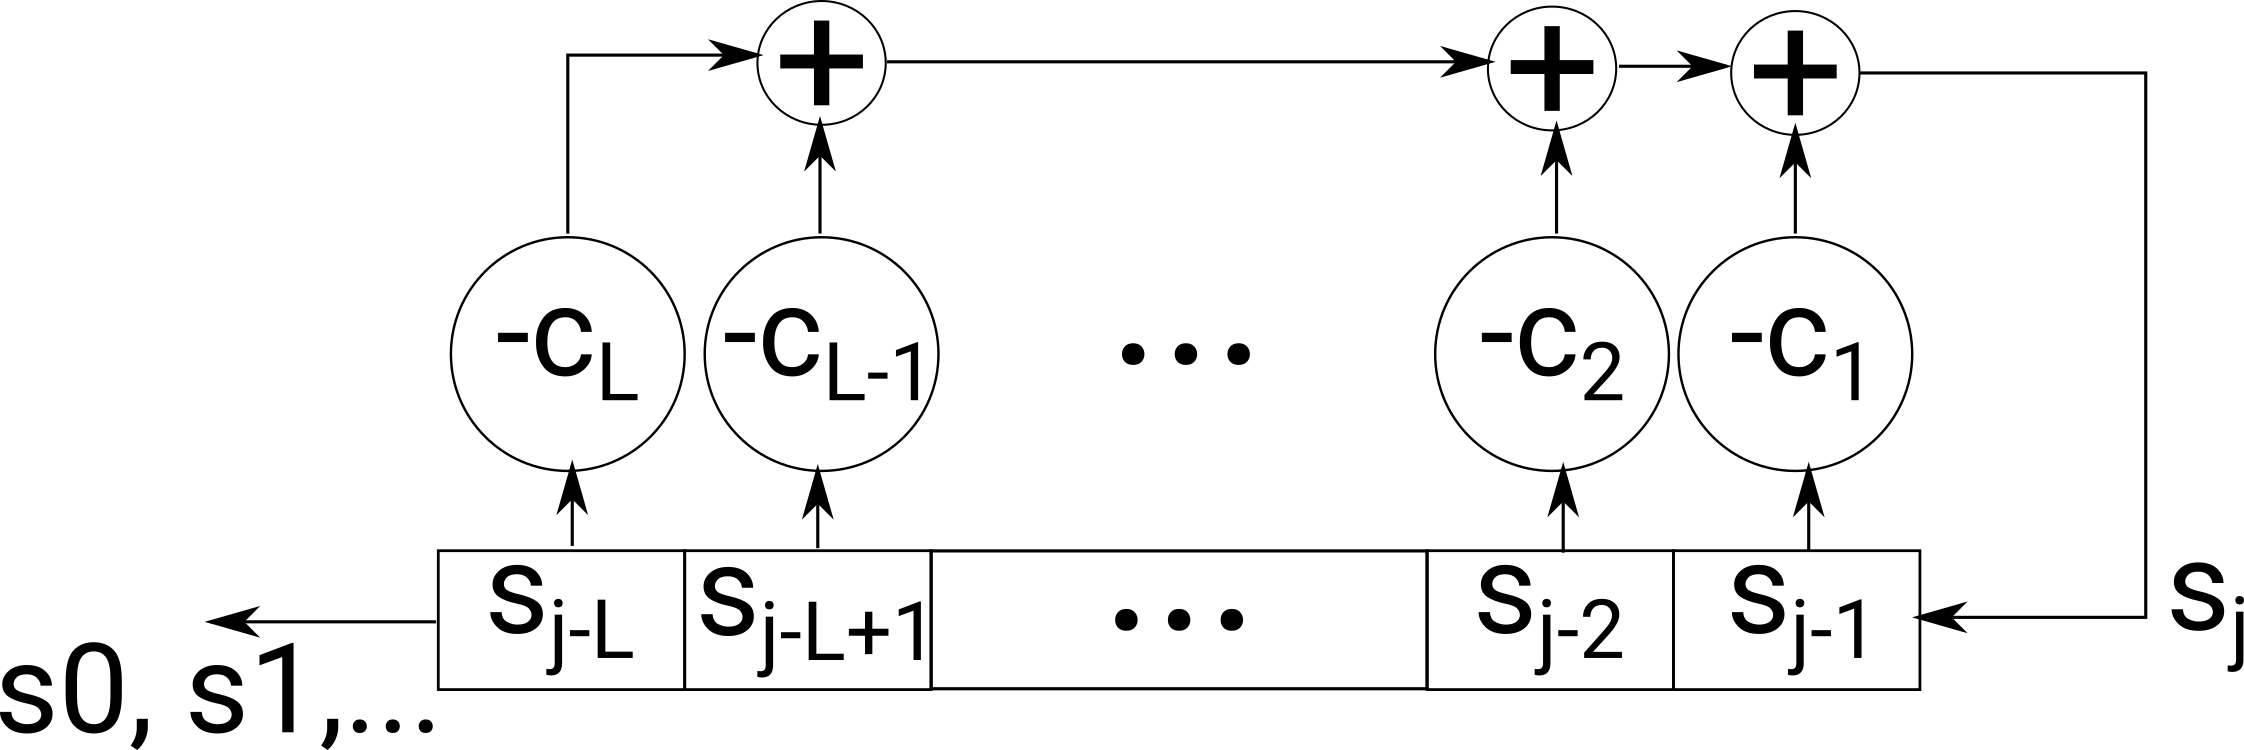
\includegraphics[scale=0.50]{./Drawings/EDIN01-Cryptography/Linear_Feedback_Shift_Register.png}
    \caption{\nameref{def:LFSR}}
    \label{fig:LSFR}
  \end{figure}
\end{definition}

\begin{definition}[Shift Register Equation]\label{def:Shift_Register_Equation}
  The \emph{shift register equation} is a way of describing the coefficients, $c_{1}, c_{2}, \ldots, c_{L} \in \FiniteMathField{F}{q}{}$, and their recurrence relation
  \begin{equation}\label{eq:Shift_Register_Equation}
    s_{j} = -c_{1}s_{j-1} - c_{2}s_{j-2} - \cdots - c_{L}s_{j-L}
  \end{equation}
  for $j = L, L+1, \ldots$.

  If  $c_{0} = 1$, we can write
  \begin{equation}\label{eq:Shift_Register_Equation-Summation}
    \sum\limits_{i=0}^{L} c_{i}s_{j-i} = 0, \text{ for } j = L, L+1, \ldots
  \end{equation}

  \begin{remark}[Initial State]\label{rmk:Shift_Register_Initial_State-Fibonacci}
    The first $L$ symbols, $s_{0}, s_{1}, \ldots, s_{L-1}$ form the \emph{initial state}.
  \end{remark}

  \begin{remark}[Fibonacci Implementation]\label{rmk:Shift_Register-Fibonacci}
    The \nameref{def:LFSR} setup shown in \Cref{fig:LSFR} is implemented in a \emph{fibonacci}-style.
  \end{remark}
\end{definition}

%%% Local Variables:
%%% mode: latex
%%% TeX-master: "../EDIN01-Cryptography-Reference_Sheet"
%%% End:


\section{Block Ciphers}\label{sec:Block_Ciphers}
\begin{definition}[Block Cipher]\label{def:Block_Cipher}
  A \emph{block cipher} encrypts a fixed-length block of plaintext bits $x$ to a fixed-length block of ciphertext $y$.
  This transformation is controlled by the secret key $K$, and is written $E_{K}(x) = y$.

  The secret key defines a fixed mapping of the plaintext block $x$ to the ciphertext block $y$.
  This can sometimes make block ciphers a form of \nameref{subsec:Simple_Substitution_Cipher}.

  Block ciphers are usually implemented with several \nameref{def:Round_Function}s, based on the \nameref{def:Round_Key}.
\end{definition}

\begin{definition}[Round Function]\label{def:Round_Function}
  \nameref{def:Block_Cipher}s are usually implemented as iterated ciphers, where a simple encryption function is iteratively applied for $N$ rounds.
  This is called a \emph{round function}.
  It is commonly denoted
  \begin{equation}\label{eq:Round_Function}
    h(w_{i-1}, k_{i})
  \end{equation}
  where
  \begin{itemize}[noitemsep]
  \item $i$ is the current round (current iteration).
  \item $w$ is the input plaintext block.
  \item $k$ is the \nameref{def:Round_Key} on the $i$th iteration.
  \item $h$ is the \nameref{def:Round_Function}.
  \end{itemize}

  These functions must also be invertible, namely,
  \begin{equation}\label{eq:Round_Function_Invertible}
    h^{-1} \bigl( h(w_{i-1}, k_{i}), k_{i} \bigr) = w_{i-1}
  \end{equation}

  \textbf{These functions must be efficient to compute, and be efficient to compute the inverse round function.}
\end{definition}

\begin{definition}[Round Key]\label{def:Round_Key}
  The \emph{round key} is derived from the key $K$.
  The way in which the round key is derived from $K$ is called the \emph{key schedule}.
\end{definition}

If we want to mathematically illustrate the implementation of a \nameref{def:Block_Cipher}'s encryption with a iterative cipher, it is defined as:
\begin{align*}
  w_{0} &= x \\
  w_{1} &= h(w_{0}, k_{1}) \\
  w_{2} &= h(w_{1}, k_{2}) \\
        &\vdots \\
  w_{N-1} &= h(w_{N-2}, k_{N-1}) \\
  w_{N} &= h(w_{N-1}, k_{N}) \\
\end{align*}
\begin{itemize}[noitemsep]
\item $x$ is the plaintext block.
\item $w_{i}$ are intermediate values in the implementation of the iteration.
\item $w_{N}$ is the final output from the cipher.
\item $h(w_{i-1}, k_{i})$ denotes the round function.
\item $k_{i}$ is the round key used in the $i$th round.
\end{itemize}

For the same iterative cipher, the decryption function $D_{K}(y)$ is just the application of the \nameref{def:Round_Key}s in reverse order.
\begin{align*}
  w_{N} &= y \\
  w_{N-1} &= h^{-1}(w_{N}, k_{N}) \\
  w_{N-2} &= h^{-1}(w_{N-1}, k_{N-2}) \\
        &\vdots \\
  w_{1} &= h^{-1}(w_{2}, k_{2}) \\
  w_{0} &= h^{-1}(w_{1}, k_{1}) = x \\
\end{align*}

\subsection{Examples of Iterated Ciphers}\label{subsec:Examples_Iterated_Ciphers}
\subsubsection{Feistel Ciphers/DES}\label{subsubsec:Feistel_Cipher_DES}
\begin{definition}[Feistel Cipher]\label{def:Feistel_Cipher}
  A \emph{Feistel cipher} is a type of iterated cipher that is easy to implement in both hardware and software.
  However, it is not safe to use anymore.

  An example of these is the DES encryption algorithm.

  The block being run through the \nameref{def:Round_Function} is split in half; a left and right half, denoted
  \begin{equation}\label{eq:Feistel_Cipher_Block}
    w_{i} = (L_{i}, R_{i})
  \end{equation}

  The \nameref{def:Round_Function} $h(L_{i-1}, R_{i-1}, k_{i})$ is implemented as
  \begin{equation}\label{eq:Feistel_Cipher_Round_Function_Encryption}
    \begin{aligned}
      L_{i} &= R_{i-1} \\
      R_{i} &= L_{i-1} \XOR f(R_{i-1}, k_{i})
    \end{aligned}
  \end{equation}
  where $f(R_{i-1}, k_{i})$ can be any function.

  The decryption function for the Feistel cipher is implemented as
  \begin{equation}\label{eq:Feistel_Cipher_Round_Function_Decryption}
    \begin{aligned}
      L_{i-1} &= R_{i} \XOR f(R_{i-1}, k_{i}) \\
      R_{i-1} &= L_{i}
    \end{aligned}
  \end{equation}
  and $(L_{0}, R_{0})$ gives back $x$.
\end{definition}

\subsubsection{SP Network}\label{subsubsec:SP_Network}
\begin{definition}[SP Network]\label{def:SP_Network}
  An \emph{SP network} is a iterated \nameref{def:Block_Cipher} that consists of a mix between substitutions (\emph{S}) (\nameref{subsec:Simple_Substitution_Cipher}s) and permutations (\emph{P}) or linear transformations (~\pageref{subsubsec:Transposition_Cipher}s).
  The \nameref{def:Round_Key} is added to the input to the \nameref{def:Round_Function} in a simple way ($\XOR$).

  An example of these is the AES (Advanced Encryption Scheme) cipher.
\end{definition}

\begin{definition}[S-Box]\label{def:S_Box}
  An \emph{S-Box} is the substitution portion of an \nameref{def:SP_Network}.
  They are usually taken over a small alphabet, and only have 4, 6, or 8 bits as input.
\end{definition}

\subsection{Modes of Operation}\label{subsec:Modes_of_Operation}
\begin{definition}[Mode of Operation]\label{def:Mode_of_Operation}
  A \emph{mode of operation} describes how to repeatedly apply a cipher's single-block operation to securely transform amounts of data larger than a block.
  This is helpful because, by themselves, \nameref{def:Block_Cipher}s can only encrypt/decrypt one block.
  To accomplish this, the plaintext is split up into blocks, and each block is encrypted.
  \begin{equation*}
    x_{1}, x_{2}, \ldots, x_{N}, x_{N+1}, \ldots
  \end{equation*}

  Let $X_{1} = (x_{1}, x_{2}, \ldots, x_{N})$ be the first block with length $N$.
  Let $X_{2} = (x_{N+1}, x_{N+2}, \ldots, x_{2N})$ be the second block, also with length $N$.
  The encryption is then done blockwise
  
  Most modes require a unique binary sequence, often called an \nameref{def:Initialization_Vector} (IV), for each encryption operation.

  There are 3 modes of operation that are discussed in this course:
  \begin{enumerate}[noitemsep]
  \item \nameref{subsubsec:Electronic_Codebook_Mode}
  \item \nameref{subsubsec:Cipher_Block_Chaining_Mode}
  \item \nameref{subsubsec:Counter_Mode}
  \end{enumerate}
\end{definition}

\begin{definition}[Initialization Vector]\label{def:Initialization_Vector}
  An \emph{initialization vector} (\emph{IV}) is a unique binary sequence that is used for each encryption operation.
  The IV has to be non-repeating and, for some modes, random as well.
\end{definition}

\subsubsection{Electronic Codebook (ECB) Mode}\label{subsubsec:Electronic_Codebook_Mode}
\begin{equation}\label{eq:Electronic_Codebook_Mode_Encryption}
  C_{I} = E_{K}(X_{i}) \:\: i=1, 2, \ldots
\end{equation}

The steps required to operate a block cipher in ECB mode are illustrated in \Crefrange{subfig:ECB_Mode_Steps_Encryption}{subfig:ECB_Mode_Steps_Decryption}.
\begin{figure}[ht!]
  \centering
  \begin{subfigure}[h!]{0.45\linewidth}
    \centering
    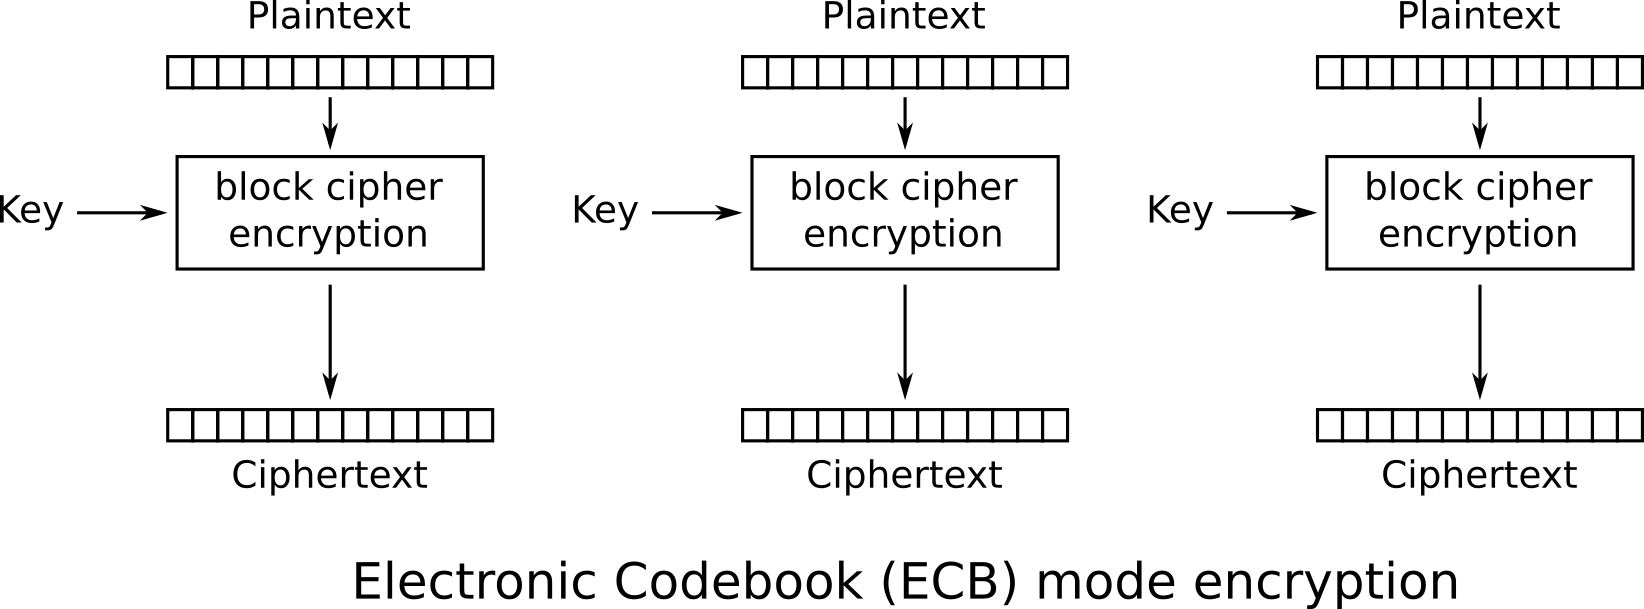
\includegraphics[scale=0.55]{./Drawings/EDIN01-Cryptography/ECB_Mode-Encryption.png}
    \caption{\nameref{subsubsec:Electronic_Codebook_Mode} Encryption Steps}
    \label{subfig:ECB_Mode_Steps_Encryption}
  \end{subfigure}
  \vline{}
  \begin{subfigure}[h!]{0.45\linewidth}
    \centering
    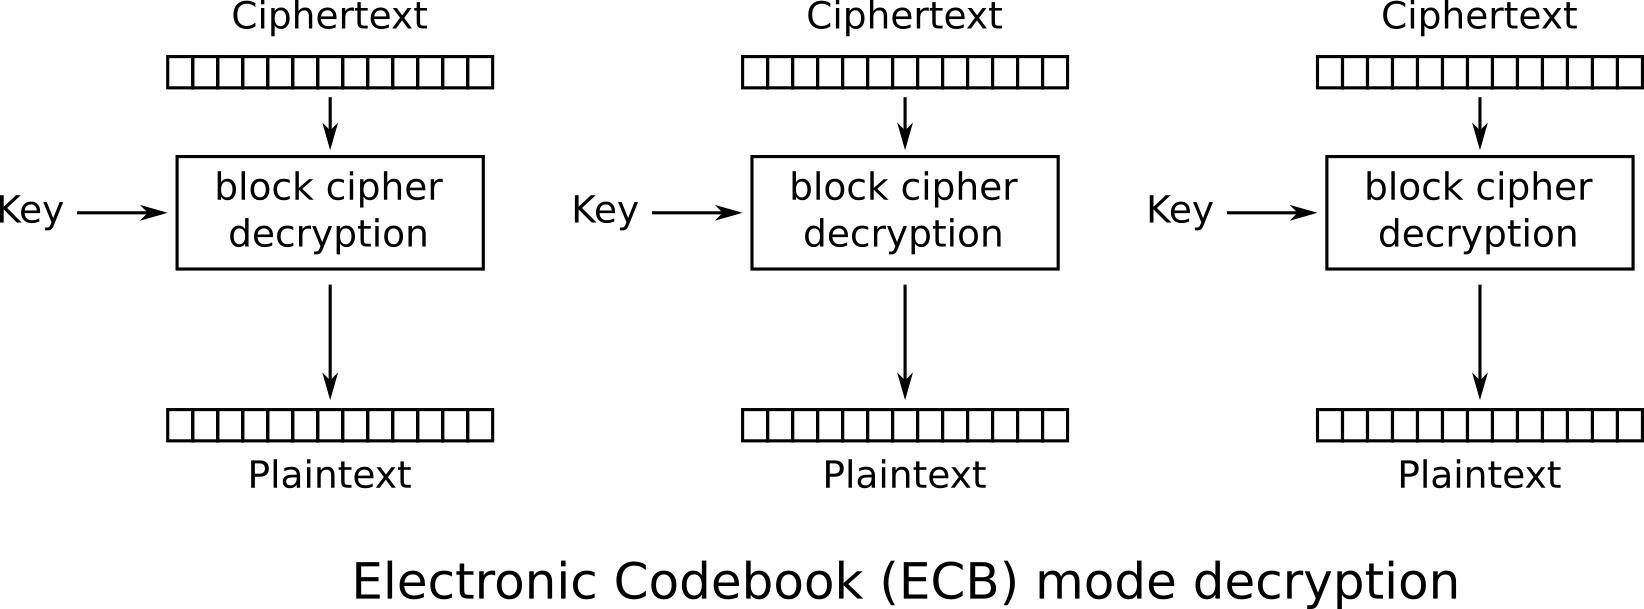
\includegraphics[scale=0.55]{./Drawings/EDIN01-Cryptography/ECB_Mode-Decryption.png}
    \caption{\nameref{subsubsec:Electronic_Codebook_Mode} Decryption Steps}
    \label{subfig:ECB_Mode_Steps_Decryption}
  \end{subfigure}
  \caption{\nameref*{subsubsec:Electronic_Codebook_Mode} Steps}
  \label{fig:Electronic_Codebook_Mode_Steps}
\end{figure}

\paragraph{Problems with \nameref*{subsubsec:Electronic_Codebook_Mode}}\label{par:Problems_Electronic_Codebook_Mode}
If 2 plaintext blocks are the same, then the 2 corresponding ciphertext blocks are \emph{also} the same.
For example,
\begin{figure}[ht!]
  \centering
  \begin{subfigure}[h!]{0.45\linewidth}
    \centering
    
\includegraphics[scale=0.50]{./Drawings/EDIN01-Cryptography/Tux.png}
    \caption{Original Plaintext}
    \label{subfig:ECB_Mode_Plaintext_Input}
  \end{subfigure}
  \begin{subfigure}[h!]{0.45\linewidth}
    \centering
    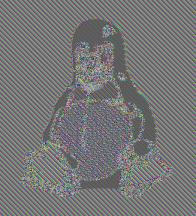
\includegraphics[scale=0.55]{./Drawings/EDIN01-Cryptography/Tux_ECB.jpg}
    \caption{ECB Mode Encrypted Plaintext}
    \label{subfig:ECB_Mode_Encrypted_Plaintext}
  \end{subfigure}
  \caption{Problem with ECB Mode}
  \label{fig:Problem_Electronic_Codebook_Mode}
\end{figure}

Notice how one could still make out the outline of the image in \Cref{subfig:ECB_Mode_Encrypted_Plaintext}.
This is undesirable, because some information is still leaked to the attacker, even after encryption.
Obviously, we need something better than ECB Mode.

\subsection{Advanced Encryption Scheme}\label{subsec:AES}
\textbf{TODO}
\begin{definition}[Advanced Encryption Scheme]\label{def:AES}
  \textbf{TODO}
\end{definition}

%%% Local Variables:
%%% mode: latex
%%% TeX-master: "../EDIN01-Cryptography-Reference_Sheet"
%%% End:


\section{Public-Key Encryption}\label{sec:Public_Key_Encryption}
\begin{definition}[Public-Key Encryption Scheme]\label{def:Public_Key_Encryption_Scheme}
  A public-key encryption scheme is a set of encryption transformations $\lbrace E_{e} : e \in \Keyspace \rbrace$ and a set of decryption transformations $\lbrace D_{d} : d \in \Keyspace \rbrace$.
  For each $e \in \Keyspace$ there is a corresponding $d \in \Keyspace$ such that $D_{d} \bigl(E_{e} (M) \bigr) = M,  \forall M$.

  Furthermore, after choosing such a pair $(e, d)$, the \emph{public key} $e$ (or the \emph{public parameter}) is made public, while the associated \emph{secret key} $d$ is kept secret.
  For the scheme to be secure, it must be computationally infeasible to compute $d$ and/or $E_{e}^{-1}(C)$, knowing the public value $e$.
  These types of schemes are built with \nameref{def:One_Way_Function}s and/or \nameref{def:Trapdoor_One_Way_Function}s.

  This means that the encryption key can be public, allowing anyone to send an encrypted message to the receiver.
  Then, only the receiver can decrypt the message, because the decryption key is kept secret.

  \begin{remark}[Construction]
    These are constructed through multiple \nameref{def:Trapdoor_One_Way_Function}s.
  \end{remark}
\end{definition}

\begin{definition}[One-Way Function]\label{def:One_Way_Function}
  An informal definition of a \emph{one-way function} $f(x)$ is a function from a set $\mathcal{X}$ to a set $\mathcal{Y}$ such that $f(x)$ is easy to compute for all $x \in \mathcal{X}$, but for ``essentially all'' elements $y \in \mathcal{Y}$ it is ``computationally infeasible'' to find any $x \in \mathcal{X}$ such that $f(x) = y$.

  \begin{remark}[``Essentially All'']\label{rmk:One_Way_Function-Essentially_All}
    There are some special values where \nameref{def:One_Way_Function}s to not behave normally, in that the function becomes computationally feasible to solve.
  \end{remark}
\end{definition}

\begin{definition}[Trapdoor One-Way Function]\label{def:Trapdoor_One_Way_Function}
  A \emph{trapdoor one-way function} $f(x)$ is a \nameref{def:One_Way_Function} $f : \mathcal{X} \mapsto \mathcal{Y}$ such that if one knows some specific information $T$, called the \emph{trapdoor information}, then $f(x)$ is computationally easy to invert $f$, i.e., for any $y \in \mathcal{Y}$ it is easy to find a $x \in \mathcal{X}$ such that $f(x) = y$.
  For anyone without knowledge of the trapdoor information $T$, $f(x)$ is a \nameref{def:One_Way_Function}.
\end{definition}

\subsection{RSA Public-Key Encryption Scheme}\label{subsec:RSA_Public_Key_Encryption_Scheme}
\begin{definition}[RSA Public-Key Encryption Scheme]\label{def:RSA_Public_Key_Encryption_Scheme}
  The \emph{RSA public-key encryption scheme} is defined as follows.
  Let $n = pq$, where $p$ and $q$ are two large \nameref{def:Prime}s.
  Let $\Messages = \Ciphertexts = \IntsMod{n}$.
  Pick a number $e$ that is \nameref{def:Relatively_Prime} to $\phi(n)$ (the \nameref{def:Set_Order} of \TextIntsMod{n}) and calculate a number $d$ such that $ed = 1 \bmod \phi(n)$.
  The \emph{public key} is the \underline{two numbers} $(n, e)$ and the public encryption transformation $E(M)$ is
  \begin{equation}\label{eq:RSA_Public_Key_Encryption_Scheme-Encryption}
    E(M) = M^{e} \bmod n
  \end{equation}

  and the associated decryption transformation is
  \begin{equation}
    \label{eq:RSA_Public_Key_Encryption_Scheme-Decryption}
    D(C) = C^{d} \bmod n
  \end{equation}
\end{definition}

\begin{proof}[RSA Public-Key Encryption Scheme]\label{proof:RSA_Public_Key_Encryption_Scheme}
  To verify that the \nameref{def:RSA_Public_Key_Encryption_Scheme} returns the plaintext after it was encrypted by the public key, we first assume that $n$, $e$, and $d$ are all properly defined.
  By extension, this means that $E(M)$ and $D(C)$ are also well-defined.

  We start be substituting the ciphertext, $C$ in \Cref{eq:RSA_Public_Key_Encryption_Scheme-Decryption} with the definition of the cipher text.
  \begin{equation*}
    \begin{aligned}
      D(C) &= C^{d} \bmod n \\
      &= {(M^{e})}^{d} \bmod n \\
      &= M^{ed} \bmod n
    \end{aligned}
  \end{equation*}

  Now, we note that $ed = 1 \bmod \phi(n)$, which means we can write
  \begin{equation*}
    ed = 1 + t \phi(n)
  \end{equation*}
  for some integer $t$.

  So, we continue, and use our two equations together.
  \begin{equation*}
    \begin{aligned}
      D(C) &= M^{ed} \bmod n \\
      &= M^{1 + \phi(n)} \bmod n \\
      &= M \cdot M^{\phi(n)} \bmod n \\
    \end{aligned}
  \end{equation*}

  From Euler's formula, we know $x^{\phi(n)} = 1$ for any $x \in \MultiplicativeGroup{n}$ (From \Cref{def:Multiplicative_Inverse} of \nameref{def:Multiplicative_Inverse}).
  We also assume that $M$ is invertible, otherwise the entire scheme falls apart, since a non-invertible message means it cannot be decrypted once encrypted.
  \begin{equation*}
    \begin{aligned}
      D(C) &= M \cdot M^{\phi(n)} \bmod n \\
      &= (M \cdot 1) \bmod n \\
      &= M \bmod n
    \end{aligned}
  \end{equation*}
\end{proof}

\begin{example}[Lecture 12, Example 3]{RSA Public-Key Encryption Scheme}
  Let $p = 47$ and $q = 167$.
  Then, $n = pq = 7849$.
  Compute $\phi(n)$,
  \begin{equation*}
    \begin{aligned}
      \phi(n) &= \phi(7849) \\
      &= \phi(47 \cdot 167) \\
      &= (47 - 1) (167 - 1) \\
      &= 7636
    \end{aligned}
  \end{equation*}

  Now, we choose a value of $e$ such that $e$ and $\phi(n)$ are \nameref{def:Relatively_Prime}, $\gcd(e, \phi(n)) = 1$.
  We choose $e=25$. (This is just one correct $e$. There are many more.)
  Since we chose $e$ where $\gcd(e, \phi(n)) = 1$, $e$ is a \nameref{def:Multiplicative_Inverse} in $\IntsMod{\phi(n)} = \IntsMod{7636}$.

  We can use the \nameref{def:Euclidean_Algorithm} and Bezout's lemma to find the inverse.
  \begin{equation*}
    d = 2749
  \end{equation*}

  Thus,
  \begin{equation*}
    25 \cdot 2749 = 1 \bmod 7636
  \end{equation*}

  Since this is true, we publish our public key, $(n, e) = (7636, 25)$.
  \tcblower{}
  Now, to send a message, Alice uses \Cref{eq:RSA_Public_Key_Encryption_Scheme-Encryption}.
  Her message has $M = 2728$.
  \begin{equation*}
    \begin{aligned}
      C &= M^{e} \bmod n \\
      &= 2728^{25} \bmod 7849 \\
      &= 2401 \bmod 7849
    \end{aligned}
  \end{equation*}

  When Bob receives this ciphertext, he can decrypt it using \Cref{eq:RSA_Public_Key_Encryption_Scheme-Decryption}.
  \begin{equation*}
    \begin{aligned}
      M &= C^{d} \bmod n \\
      &= 2401^{2749} \bmod 7849 \\
      &= 2728 \bmod 7849
    \end{aligned}
  \end{equation*}

  Thus, Bob gets Alice's original message, and he is likely the only one who was able to decrypt it.
\end{example}

\subsubsection{Security of the \nameref*{subsec:RSA_Public_Key_Encryption_Scheme}}\label{subsubsec:RSA_Encryption_Scheme-Security}
The \nameref{def:RSA_Public_Key_Encryption_Scheme} relies on the factorization problem.
Namely, that for large semi-prime numbers, it is difficult to find its constiuent \nameref{def:Prime} factors.
However, this \textbf{does not} mean that breaking RSA is equivalent to solving a factorization problem.
It is currently unknown if there is a way to break RSA without factoring the integer $n$.

\subsubsection{Implementation of the \nameref*{subsec:RSA_Public_Key_Encryption_Scheme}}\label{subsubsec:RSA_Encryption_Scheme-Implementation}
In order to compute $M^{e} \bmod n$ we need $L = \lceil \log_{2} n \rceil$ bits to store a value from \TextIntsMod{n}.

To easily compute the exponentiation of $M$ with $e$, we apply the \emph{square and multiply algorithm}.
\begin{definition}[Square and Multiply Algorithm]\label{def:Square_Multiply_Algorithm}
  The \emph{square and multiply algorithm} is a way to efficiently compute exponents.
  If the expression in question is $M^{e}$, we first rewrite $e$ as a sum of powers of 2.
  \begin{equation*}
    e = e_{0} + e_{1} \cdot 2 + e_{2} \cdot 2^{2} + \cdots + e_{L-1} w^{L-1}
  \end{equation*}
  where $e_{i} \in \IntsMod{2}$ and $0 \leq i \leq L-1$.

  Next, $L-1$ squarings of $M$ occurs.
  \begin{equation*}
    M^{2}, \Bigl( M^{4} = {\left( M^{2} \right)}^{2} \Bigr), \Bigl( M^{4} = {\left( M^{4} \right)}^{2} \Bigr), \ldots
  \end{equation*}
  in \TextIntsMod{n} (i.e.\ reducing modulo $n$ every time).

  Lastly, we perform at most $L-1$ multiplications by computing $M^{e}$ as
  \begin{equation*}
    M^{e} = M^{e_{0}} \cdot {\left( M^{2} \right)}^{e_{1}} \cdot {\left( M^{4} \right)}^{e_{2}} \cdots {\left( M^{2^{L-1}} \right)}^{e_{L-1}}
  \end{equation*}
\end{definition}

\begin{example}[Lecture 14, Example 1]{Square and Multiply Algorithm}
  Compute $2728^{25}$ in \TextIntsMod{7849} using the \nameref{def:Square_Multiply_Algorithm}?
  \tcblower{}
  First, rewrite 25 as a result of products of 2.
  \begin{align*}
    25 &= 16 + 8 + 1 \\
    &= 1 (2^{4}) + 1 (2^{3}) + 0 (2^{2}) + 1 (2^{1}) + 1 (2^{0})
  \end{align*}
  This results in
  \begin{equation*}
    2728^{25} = 2728^{1} \cdot 2728^{8} \cdot 2728^{16}
  \end{equation*}

  Now we perform the squarings required until we get to $2728^{16}$.
  \begin{align*}
    2728^{2} &= 7441984 \bmod 7849 = 1132 \\
    2728^{4} &= {(2728^{2})}^{2} = 1132^{2} \bmod 7849 = 2037 \\
    2728^{8} &= {(2728^{4})}^{2} = 2037^{2} \bmod 7849 = 5097 \\
    2728^{16} &= {(2728^{8})}^{2} = 5097^{2} \bmod 7849 = 7068
  \end{align*}

  Now substituting our values in and multiplying through (ensuring we reduce modulo $n$ at the end).
  \begin{align*}
    2728^{25} &= 2728^{16+8+1} \\
              &= (2728 \cdot 5097 \cdot 7068) \bmod 7849 \\
              &= 2401
  \end{align*}

  Our answer is $2728^{25} \bmod 7849 = 2401$.
\end{example}

\subsection{Primality Testing}\label{subsec:Primality_Testing}
How do we check whether a given number $m$ is a \nameref{def:Prime} number?

The na\"{\i}ve approach said to perform trial divisions such that $x \Divides m$ for all integers $x$ where $2 \leq x \leq \sqrt{m}$.
The problem with this is that if $m$ is a 1024-bit number, for instance, then $\sqrt{m}$ is 512-bits, and performing $2^{512}$ tests is not possible.

So, we have probabilistic theorems for determining primality of numbers.

\subsubsection{Probabilistic Algorithms for Testing Primality}\label{subsubsec:Probabilistic_Algorithms_Testing_Primality}
\paragraph{Fermat's Little Theorem}\label{par:Fermats_Little_Theorem}
\begin{theorem}[Fermat's Little Theorem]\label{thm:Fermats_Little_Theorem}
  Fermat's Little Theorem states that
  \begin{equation}\label{eq:Fermats_Little_Theorem}
    a^{m-1} = 1 \bmod m
  \end{equation}
  if $m$ is a \nameref{def:Prime} and $a$ such that $1 \leq a \leq m-1$.

  When $m$ is not a \nameref{def:Prime}, we cannot know what we will receive when computing $a^{m-1}$.
  However, if $a^{m-1} \neq 1 \bmod m$, we know \textbf{for certain} that $m$ is \textbf{not} a \nameref{def:Prime} number.
\end{theorem}

\begin{remark*}[Error Probability of \nameref{thm:Fermats_Little_Theorem}]
  The error probability after repeating the test $k$ times would be less than $\frac{1}{2^{k}}$.
\end{remark*}

\begin{definition}[Pseudo-Prime]\label{def:Pseudo_Prime}
  A composite $m$ such that $a^{m-1} = 1 \bmod m$ is said to be a \emph{pseudo-prime} to the base $a$.
\end{definition}

\begin{definition}[Carmichael Number]\label{def:Carmichael_Number}
  A number is called a \emph{Carmichael number} if a composite $m$ is such that it is a \nameref{def:Pseudo_Prime} for every base $a$ with $\gcd(a, m) = 1$.

  \begin{remark}[Smallest \nameref*{def:Carmichael_Number}]
    The smallest \nameref{def:Carmichael_Number} is 561.
  \end{remark}
\end{definition}

\begin{theorem}[Miller-Rabin Test]\label{thm:Miller_Rabin_Test}
  The Miller-Rabin test states that we choose a random integer as base, $a$.
  Then write $m -1 = 2^{b} \cdot q$, where $q$ is odd.

  If $a^{q} = 1 \bmod m$ or $a^{2^{c} \cdot q} = -1 \bmod m$ for any $c < b$ then return ``$m$ probably \nameref{def:Prime}'' and go back and choose a new base.
  Otherwise, return ``$m$ is definitely \textbf{not} \nameref{def:Prime}''.

  One can prove that the probability that $m$ is probably \nameref{def:Prime} with to the below equation.
  \begin{equation}\label{eq:Miller_Rabin_Test_Success_Probability}
    \Prob \left( \text{``$m$ probably prime''} \Given \text{``$m$ not prime''} \right) < \frac{1}{4}
  \end{equation}
\end{theorem}

\subsection{Factoring}\label{subsec:Factoring}
All \nameref{def:Public_Key_Encryption_Scheme}s used today rely on the intractability of factoring large semi-primes.

\subsubsection{\texorpdfstring{Pollard's $(p-1)$-Method}{Pollard's Method}}\label{subsubsec:Pollards_Method}
\begin{theorem}[\texorpdfstring{Pollard's $(p-1)$-Method}{Pollard's Method}]\label{thm:Pollards_Method}
  Let $n = pq$ and let $p-1$ factor as
  \begin{equation*}
    p-1 = q_{1}q_{2} \cdots q_{k}
  \end{equation*}
  where each $q_{i}$ is a \nameref{def:Prime} power.

  There is a condition where each $q_{i} < B$ where $B$ is a predetermined ``bound''.
  If this condition is valid, then we have
  \begin{equation*}
    (p-1) \Divides B!
  \end{equation*}

  We compute $a = 2^{B!} \bmod n$.
  Now let $a' = 2^{B!} \bmod p$.
  Since $p \Divides n$, we must have $a \bmod p = a'$.

  \nameref{thm:Fermats_Little_Theorem} states that
  \begin{equation*}
    2^{p-1} = 1 \bmod p
  \end{equation*}
  and since $(p-1) \Divides B!$, we also have $a' = 1 \bmod p$, which leads to $a = 1 \bmod p$.

  So, $p \Divides (a-1)$ and since $p \Divides n$, we also have $p = \gcd(a-1, n)$.
\end{theorem}

The algorithm stands as:
\begin{enumerate}[noitemsep]
\item Compute $a^{2B!} \bmod n$.
\item Compute the unknown prime $p$ as $p = \gcd(a-1, n)$.
\end{enumerate}

An important conclusion to draw here is that the \nameref{def:Prime}s $p$ and $q$ must be chosen such that $p-1$ and $q-1$ each contains a large \nameref{def:Prime} in their factorization.
The usual approach is to generate a random \nameref{def:Prime} $p_{1}$ and test whether $p = 2p_{1} + 1$ is a prime number.
If so, we choose $p$.

\subsubsection{Other Factoring Methods}\label{subsubsec:Other_Factoring_Methods}
There are many modern factoring methods that are more efficient than \nameref{thm:Pollards_Method}.
\begin{enumerate}[noitemsep]
\item Quadratic Sieve
\item Number Field Sieve
\item Elliptic Curve Factorization
\item Pollard's Rho Algorithm Method
\item etc.
\end{enumerate}

\subsubsection{Computational Complexity of Factoring}\label{subsubsec:Factoring_Computational_Complexity}
We often use the function to model complexity of algorithms with sub-exponential behavior.
\begin{equation}\label{eq:Sub_Exponential_Behavior}
  L_{N}(\alpha, \beta) = e^{\bigl( \beta + O(1){(\log(N))}^{\alpha} {\log(\log(N))}^{1-\alpha}\bigr)}
\end{equation}

Number field sieves are currently the most successful method for factoring semi-\nameref{def:Prime} numbers with more than 100 decimal digits.
It can factor numbers of the size $2^{512}$
Its complexity behavior is sub-exponential, with $L_{N}(\frac{1}{3}, 1.923)$.

\subsection{Uses of Public-Key Cryptography}\label{subsec:Uses_Public_Key_Cryptography}
There are 3 basic \nameref{def:Cryptographic_Primitive}s that \nameref{def:Public_Key_Encryption_Scheme}s are used for.
\begin{enumerate}[noitemsep]
\item \nameref{def:Public_Key_Encryption_Scheme}: A messis encrypted with a recipient’s public key and cannot be decrypted by anyone except the recipient possessing the private key.
\item \nameref{subsec:Digital_Signatures}: A message signed with a sender’s private key can be verified by anyone who has access to the sender’s public key, thereby proving that the correct original sender signed it and that the message has not been tampered with during message transmission (authenticity and nonrepudiation).
\item \nameref{subsec:Key_Exchange}: A cryptographic protocol that allows two parties that have no prior knowledge of each other to jointly establish a shared secret key.
\end{enumerate}

The major problem with using a public key is linking it an entity or principal.
The most common solution to this problem is the use of a \nameref{def:Digital_Certificate}.

\begin{definition}[Digital Certificate]\label{def:Digital_Certificate}
  A \emph{digital certificate} is a ``stamp of approval'' that the public key belongs to who the principal says it belongs to.
  There is a third-party called a \nameref{def:Certificate_Authority} that handles the signing of entity's/principal's public keys to ensure they are authentic.

  A digital certificate has the form of
  \begin{center}
    (Alice, $\ldots$, Alice's public key, CA's signature)
  \end{center}
\end{definition}

\begin{definition}[Certificate Authority]\label{def:Certificate_Authority}
  A \emph{certificate authority} or (\emph{CA}) is a third-party that vouches for the validity of the public keys in use by an entity/principal.
\end{definition}

\subsubsection{Digital Certificates and Certificate Authorities}\label{subsubsec:Digital_Certificate_Certificate_Authorities}
A \nameref{def:Certificate_Authority}-based system works by establishing a ``web of trust''.
\begin{enumerate}[noitemsep]
\item All users have a trusted copy of the public key of the \textbf{\nameref{def:Certificate_Authority}}. For example, these are embedded in your web browser.
\item The \nameref{def:Certificate_Authority} signs data strings containing the following information.
  \begin{center}
    (Alice, $\ldots$, Alice's public key, CA's signature)
  \end{center}
  This data string and the associated signature is called a \nameref{def:Digital_Certificate}.
  The \nameref{def:Certificate_Authority} only signs the data if it believes the public key really belongs to Alice.
\item When Alice sends her public key, contained in the digital certificate, you now trust that the public key is really Alice's, since you trust the \nameref{def:Certificate_Authority} and you checked their signature too.
\end{enumerate}

\subsection{The Discrete Logarithm Problem}\label{subsec:Discrete_Log_Problem}
\begin{definition}[Discrete Logarithm Problem]\label{def:Discrete_Log_Problem}
  Let $(G, *)$ be an \nameref{def:Abelian} \nameref{def:Group}.
  The \emph{discrete logarithm problem} states that given $g, h \in G$, find an $x$ (if it exists) such that $g^{x} = h$.

  The difficulty of this problem depends on the group $G$ chosen.
  \begin{itemize}[noitemsep]
  \item Very Easy: Polynomial Time Algorithm. $(\IntsModN{}, +)$
  \item Hard: Sub-Exponential Time Algorithm. $(\FiniteMathField{F}{p}{*})$
  \item Very Hard: Exponential Time Algorithm. Elliptic Curve Groups (Not discussed in this course).
  \end{itemize}
\end{definition}

\subsection{Key Exchange}\label{subsec:Key_Exchange}
\begin{definition}[Key Exchange]\label{def:Key_Exchange}
  \emph{Key exchange} is a cryptographic protocol that allows two parties that have no prior knowledge of each other to jointly establish a shared secret key.
\end{definition}

\subsubsection{Diffie Hellman Key Exchange}\label{subsubsec:Diffie_Hellman_Key_Exchange}
\begin{definition}[Diffie Hellman Key Exchange]\label{def:Diffie_Hellman_Key_Exchange}
  The \emph{Diffie Hellman Key Exchange} is a type of \nameref{def:Key_Exchange} that allows 2 parties to agree to a secret key over an insecure channel without having met before.

  Let $G = \FiniteMathField{F}{p}{*}$ and $g \in \FiniteMathField{F}{p}{*}$.
  The basic message flows for this protocol is:
  \begin{enumerate}[noitemsep]
  \item Alice selects a secret $a$, and Bob selects a secret $b$.
  \item Alice sends $A = g^{a} \bmod p$ to Bob.
  \item Bob sends $B = g^{b} \bmod p$ to Alice.
  \item Alice computes $K_{A} = B^{a} \bmod p = g^{b^{a}} = g^{ba}$.
  \item Bob computes $K_{B} = A^{b} \bmod p= g^{a^{b}} = g^{ab}$.
  \item If both $K_{A} = K_{B}$, then the secret key has been created for Alice and Bob.
  \end{enumerate}

  \begin{remark}[Flaws in \nameref*{def:Diffie_Hellman_Key_Exchange}]\label{rmk:Flaws_Diffie_Hellman_Key_Exchange}
    While this would work for most cases, the entire \nameref{def:Diffie_Hellman_Key_Exchange} protocol is vulnerable to a \emph{Man-in-the-Middle attack}.
  \end{remark}
\end{definition}

\begin{example}[Lecture 15, Example 1]{Diffie Hellman Key Exchange}
  Given the comain parameters $p = 2147482659$, $g = 2$ and the secret keys chosen by Alice $a = 12345$ and Bob $b = 654323$, compute their shared key?
  \tcblower{}
  \begin{align*}
    &\text{Alice} & &\text{Bob} \\
    a &= 12345 & b &=654323 \\
    A &= g^{a} = 2^{12345} \bmod 2147482659 = 428647416 & B &= g^{b} = 2^{654323} \bmod 2147482659 = 450904856 \\
    K_{A} &= B^{a} \bmod 2147482659 & K_{B} &= A^{b} \bmod 2147482659\\
    &= 450904856^{12345} \bmod 2147482659 & &= 428647416^{654323} \bmod 2147482659 \\
    &= 1333327162 & &= 1333327162
  \end{align*}

  Thus, Alice and Bob have managed to agree on a secret key of $K=1333327162$.
\end{example}

%%% Local Variables:
%%% mode: latex
%%% TeX-master: "../EDIN01-Cryptography-Reference_Sheet"
%%% End:


\section{Hash Functions}\label{sec:Hash_Functions}
\begin{definition}[Hash Function]\label{def:Hash_Function}
  A cryptographic \emph{hash function} $h$ is a function which takes \textbf{arbitrary} length bit strings as input and produces a \textbf{fixed length} bit string as output, the \emph{hash value}.
  There are a few requirements for hash functions:
  \begin{enumerate}[noitemsep]
  \item It must be a \nameref{def:One_Way_Function}
  \item \nameref{def:Preimage_Resistant}
  \item \nameref{def:Second_Preimage_Resistant}
  \item \nameref{def:Collision_Resistant}
  \end{enumerate}
\end{definition}

\begin{definition}[Preimage Resistant]\label{def:Preimage_Resistant}
  A \nameref{def:Hash_Function} given an output hash value of $n$ bits, is considered \emph{preimage resistant} if the time complexity for finding the input plaintext is $O(2^{n})$.

  \begin{remark}[Assumption of Preimage Resistance]\label{rmk:Preimage_Resistant_Assumption}
    Assuming a \nameref{def:Hash_Function} is \nameref{def:Preimage_Resistant} for almost every element of the range of $h$ is a weaker assumption than assuming it is either \nameref{def:Second_Preimage_Resistant} or \nameref{def:Collision_Resistant}.
  \end{remark}
\end{definition}

\begin{definition}[Second Preimage Resistant]\label{def:Second_Preimage_Resistant}
  A \nameref{def:Hash_Function} that is \emph{second preimage resistant} is one where given one message, it is difficult to find another message with the same hash value.

  \begin{remark}[Assumption of Second Preimage Resistance]\label{rmk:Second_Preimage_Resistant_Assumption}
    Assuming a \nameref{def:Hash_Function} is \nameref{def:Second_Preimage_Resistant} is a weaker assumption than assuming it is \nameref{def:Collision_Resistant}.
  \end{remark}
\end{definition}

\begin{definition}[Collision Resistant]\label{def:Collision_Resistant}
  A \nameref{def:Hash_Function} is \emph{collision resistant} if it is hard to find 2 plaintext messages with the exact same hash value.

  \begin{remark}[Assumption of Collision Resistance]\label{rmk:Collision_Resistant_Assumption}
    Assuming a \nameref{def:Hash_Function} is \nameref{def:Collision_Resistant} is the strongest assumption we can make about a well-crafted \nameref{def:Hash_Function}.
  \end{remark}
\end{definition}

\subsection{Usages of Hash Functions}\label{subsec:Hash_Functions_Usages}
There are several reasons to use \nameref{def:Hash_Function}s.
\begin{itemize}[noitemsep]
\item \emph{Commitment to messages} by disclosing the hash of a message, then later showing the message. This allows the hash to be checked. However, this requires a few different things.
  \begin{itemize}[noitemsep]
  \item If the \nameref{def:Hash_Function} is collision-resistant, you cannot cheat by substituting your original message for another.
  \end{itemize}
\item \emph{Verify integrity} of downloaded files
  \begin{itemize}[noitemsep]
  \item Torrents use this to make sure you download the right contents. If something goes wrong, only the right small chunk can be redownloaded.
  \end{itemize}
\item \emph{Digital signatures} for things that require confirmation of action from the user/requester.
\item \emph{SSL/TLS} for integrity protection
\item \emph{Storing passwords} in operating systems (\texttt{/etc/shadow} on *nix machines) and websites.
  \begin{itemize}[noitemsep]
  \item You can add salt to change the hash around, usually for webserver passwords. These password databases store the userid, the salt added to the password, and the hashed password. At login time, the password and random number are hashed together again, and compared.
  \end{itemize}
\end{itemize}

\subsection{Merkle-Damg\r{a}rd Construction}\label{subsec:Merkle_Damgard_Construction}
\begin{definition}[Merkle-Damg\r{a}rd Construction]\label{def:Merkle_Damgard_Construction}
  Since \nameref{def:Hash_Function}s have an essentially infinite domain, due to their arbitrary length input, designing a \nameref{def:Hash_Function} can be quite diffcult.
  However, if we break the input down into blocks, we can use a \emph{compression function} to map bits from input length $s$ into output hash values of lengths $n$.
  These compression functions can be chained together to produce a function that acts on an infinite domain.
  The chaining method most frequently used by \nameref{def:Hash_Function}s is the \emph{Merkle-Damg\r{a}rd Construction}.
\end{definition}

\begin{theorem}
  If the compression function $f$ is \nameref{def:Collision_Resistant}, then the \nameref{def:Hash_Function} $h$ is also \nameref{def:Collision_Resistant}.
\end{theorem}

\begin{definition}[Length Strengthening]\label{def:Length_Strengthening}
  The input message is preprocessed by first padding with zero bits to obtain a message which has length a multiple of $l$ bits.
  Then a final block of $l$ bits is added which encodes the original length of the unpadded message in bits.
  The construction is limited to hashing messages with length less than $2l$ bits.
\end{definition}

\subsection{SHA-1}\label{subsec:SHA_1}
The internal state of the algorithm is a set of 5 32-bit values.
\begin{equation*}
  (H_{1}, H_{2}, H_{3}, H_{4}, H_{5})
\end{equation*}
and 4 round constants
\begin{equation*}
  y_{1}, y_{2}, y_{3}, y_{4}
\end{equation*}

\nameref{def:Length_Strengthening} is used, but is slightly modified in the SHA-1 algorithm.
First, a one bit is appended to the plaintext message, to signal its end.
Then zeros are padded until the length of the plaintext message is a multiple of 512-bits.
Lastly, the number of bits of the message is appended as a separate, final, block.

\begin{algorithm}[H]
  \DontPrintSemicolon{}
  \SetKwInOut{Input}{Input}\SetKwInOut{Output}{Output}

  \Input{$(H_{1}, H_{2}, H_{3}, H_{4}, H_{5})$ and $(y_{1}, y_{2}, y_{3}, y_{4})$}
  \Output{Concatenation of $(H_{1}, H_{2}, H_{3}, H_{4}, H_{5})$}
  \BlankLine{}

  $(A, B, C, D, E) = (H_{1}, H_{2}, H_{3}, H_{4}, H_{5})$\;
  \For{$j=16$ \KwTo{} $79$}{
    $X_{j} = \bigl( (X_{j-3} \XOR X_{j-8} \XOR X_{j-14} \XOR X_{j-16}) \lll 1 \bigr)$
  }
  Execute Round 1 (\Cref{algo:SHA_1_Round_1}) \;
  Execute Round 2 (\Cref{algo:SHA_1_Round_2}) \;
  Execute Round 3 (\Cref{algo:SHA_1_Round_3}) \;
  Execute Round 4 (\Cref{algo:SHA_1_Round_4}) \;
  \caption{SHA-1 Overview}
  \label{algo:SHA_1_Overview}
\end{algorithm}


\subsection{Security Status of Various Hash Functions}\label{subsec:Hash_Functions_Security_Status}
In practice, MD5 and SHA-1 are the most common, but are also broken.
\begin{itemize}[noitemsep]
\item MD5 is broken in practice
\item SHA-1 is broken in theory, no efficient implementation has been developed yet.
\end{itemize}

There are 2 new versions of the SHA family that have not been broken yet.
\begin{enumerate}[noitemsep]
\item SHA-2
\item SHA-3
  \begin{itemize}[noitemsep]
  \item Output of an NIST competition in 2012.
  \end{itemize}
\end{enumerate}

\subsection{SHA-3}\label{subsec:SHA_3}
\begin{definition}[SHA-3]\label{def:SHA_3}
  \emph{SHA-3} uses a sponge construction, where the message blocks are XORed together into the initial bits of the state.
\end{definition}

\subsection{Message Authentication Codes}\label{subsec:MACs}
\begin{definition}[Message Authentication Code]\label{def:MAC}
  A \emph{message authentication code} is a \nameref{def:Hash_Function} that uses a key.

  \begin{remark}[Relation to \nameref*{def:Block_Cipher}s]\label{rmk:MAC_Block_Cipher_Relation}
    Many \nameref{def:Block_Cipher}s provide a \nameref{def:Mode_of_Operation} to work with \nameref{def:MAC}s.
  \end{remark}
\end{definition}

There are 2 major designs:
\begin{enumerate}[noitemsep]
\item HMAC (Based on \nameref{def:Hash_Function})
\item CBC-MAC (Based on \nameref{def:Block_Cipher} in CBC-Mode)
\end{enumerate}

There are 2 na\"{\i}ve implementations of a \nameref{def:MAC}s.
\begin{enumerate}[noitemsep]
\item
  \begin{equation*}
    \text{MAC}_{k}(m) = h(m \Vert k)
  \end{equation*}
\item
  \begin{equation*}
    \text{MAC}_{k}(m) = h(m \Vert k)
  \end{equation*}
\end{enumerate}

\subsubsection{HMAC}\label{subsubsec:HMAC}
HMAC is a MAC based on a \nameref{def:Hash_Function}.
\begin{equation}\label{eq:HMAC}
  \text{HMAC}_{k}(m) = h((k \XOR) \Vert h((k \XOR ipad) \Vert m))
\end{equation}
\begin{itemize}[noitemsep]
\item opad = $\mathtt{0x5c5c5c} \ldots$
\item ipad = $\mathtt{0x363636} \ldots$
\end{itemize}

The implementation in \Cref{eq:HMAC} was developd in 1996, and when used with MD5 and/or SHA-1, it is immune to previous attacks.

\subsubsection{Usages of Message Authentication Codes}\label{subsubsec:MAC_Usages}
\begin{itemize}[noitemsep]
\item Authenticate origin of messages
  \begin{itemize}[noitemsep]
  \item A symmetric key is shared between the sender and receiver.
  \item Both the sender and receiver can create and verify a MAC.
  \end{itemize}
\end{itemize}

%%% Local Variables:
%%% mode: latex
%%% TeX-master: "../EDIN01-Cryptography-Reference_Sheet"
%%% End:


\section{Authentication}\label{sec:Authentication}
There are 3 ways we can confirm authenticity with authentication schemes:
\begin{enumerate}[noitemsep]
\item Unconditionally Secure \nameref{subsec:Authentication_Codes}
\item \nameref{def:MAC}
\item \nameref{subsec:Digital_Signatures}
\end{enumerate}

\subsection{\nameref*{subsec:MACs} with Authentication}\label{subsec:MAC_Authentication}
\nameref{def:MAC}s can be used as an authentication technique that uses \nameref{def:Cryptographic_Primitive}s (\nameref{def:Block_Cipher}s and \nameref{def:Hash_Function}s) to provide authentication.

\begin{remark*}
  It is assumed that the sender and reciever both share the same key used for the \nameref{def:MAC}.
\end{remark*}

\subsubsection{Problems with \nameref*{subsec:MACs} and Authentication}\label{subsubsec:MAC_Problems_Authentication}
\nameref{def:MAC}s do not protect against an unlimited enemy, i.e.\ an unlimited number of attackers or an attacker with infinite computing power.
However, they are able to authenticate many messages without changing the key.

\subsubsection{CBC-MAC for Authentication}\label{subsubsec:CBC_MAC_Authentication}
CBC-MAC is a \nameref{def:Mode_of_Operation} for \nameref{def:Block_Cipher}s to operate with \nameref{def:MAC}s.
A \nameref{def:Block_Cipher} is secure for fixed-length messages, but insecure for variable-length messages.
The problem is that the same key $K$ cannot be reused anywhere.

\subsection{Digital Signatures}\label{subsec:Digital_Signatures}
This is an asymmetric (\nameref{def:Public_Key_Encryption_Scheme}) solution.
The advantages of this are:
\begin{itemize}[noitemsep]
\item No need to distribute/establish a common secret key
\item Nonrepudiation, if the receiver received an authentic message, the sender cannot deny having sending it
\end{itemize}

The disadvantages of this are:
\begin{itemize}[noitemsep]
\item Signature schemes rely on the hardness of problems, like semiprime integer factoring.
\item These signature schemes also rely on large numbers.
\item Both of these factors slow down the process of this technique compared to others.
\end{itemize}

\subsection{Authentication Codes}\label{subsec:Authentication_Codes}
\begin{definition}[Authentication Code]\label{def:Authentication_Code}
  An \emph{authentication code} is used to check if the received message was sent by the claimed sender.
  They are also used to verify that the message was not modified (by a third-party, not random errors) during transmission.

  The authentication code requires there be \emph{secret keys} that are known to the sender and receiver, but not to the enemy.

  There can be several models of authentication codes.
  In this course, we only look at \nameref{subsubsec:Authentication_Code_Unconditionally_Secure_Model}.
  The formula defining this type of authentication code is given in \Cref{eq:Unconditional_Authentication_Code}.
\end{definition}

\subsubsection{The Unconditionally Secure Model}\label{subsubsec:Authentication_Code_Unconditionally_Secure_Model}
An unconditionally secure solution is given below.
\begin{itemize}[noitemsep]
\item The transmitted information, the \emph{source message} (\nameref{def:Plaintext}) is denoted $s$ and $s \in \SourceMessages$.
\item The source message is mapped to a \emph{channel message} $m$ where $m \in \ChannelMessages$.
\item Using the secret key $k$ where $k \in \Keyspace$.
\end{itemize}

\begin{equation}\label{eq:Unconditional_Authentication_Code}
  f : \SourceMessages \times \Keyspace \rightarrow \mathcal{M} : (s, k) \mapsto m
\end{equation}
\begin{itemize}[noitemsep]
\item An important property of $f$ is that if $f(s, e) = m$ and $f(s', e) = m$, then $s = s'$ (Injective for each $k \in Keyspace$).
\item Meaning the receiver must check whether a source message $s$ even exists.
\item If such an $s$ exists, $m$ is valid.
\item Otherwise, the message $m$ is not authentic.
\end{itemize}

\begin{large}
  \textbf{The mapping $f$, along with $\SourceMessages$, $\ChannelMessages$, and $\Keyspace$ define an \nameref{def:Authentication_Code} (\emph{A-Code}).}
\end{large}

\subsubsection{Attacks on Authentication Codes}\label{subsubsec:Attacks_Authentication_Codes}
There are only 2 reasonable attacks on \nameref{def:Authentication_Code}s possible.
\begin{enumerate}[noitemsep]
\item \nameref{par:Attack_Authentication_Code-Impersonation}
\item \nameref{par:Attack_Authentication_Code-Substitution}
\end{enumerate}

\begin{definition}[Probability of Deception]\label{def:Probability_of_Deception}
  The \emph{probability of deception} is the probability that a non-authentic message is authenticated by the \nameref{def:Authentication_Code} system as a valid message.
  It is based off probabilities of success of \nameref{def:Attack_Authentication_Code-Impersonation}s and \nameref{def:Attack_Authentication_Code-Substitution}s.
  
  \begin{equation}\label{eq:Probability_of_Deception}
    \Prob_{D} = \max(\Prob_{i}, \Prob_{S})
  \end{equation}
\end{definition}

\begin{theorem}[Square Root Bound]\label{thm:Prob_Deception_Square_Root_Bound}
  By first multiplying the Simmons' Bounds on the probabilities of success of each attack, we can find their combined probability.
  Using \Cref{thm:Impersonation-Simmons_Bound} and \Cref{thm:Substitution-Simmons_Bound} and multiplying:
  \begin{equation*}
    \Prob_{I}\Prob_{S} \geq 2^{-\MutualInformation(M; K) - \Entropy(K \Given M)} = 2^{-\Entropy(K)}
  \end{equation*}

  From $\Entropy(K) \leq \log_{2} \SetOrder{\Keyspace}$ we can find the \emph{square root bound} of the \nameref{def:Probability_of_Deception} \textbf{for any \nameref{def:Authentication_Code}}.
  \begin{equation}\label{eq:Prob_Deception_Square_Root_Bound}
    \Prob_{D} \geq \frac{1}{\sqrt{\SetOrder{\Keyspace}}}
  \end{equation}
\end{theorem}

\paragraph{Impersonation Attacks}\label{par:Attack_Authentication_Code-Impersonation}
\paragraph{Substitution Attacks}\label{par:Attack_Authentication_Code-Substitution}
\subsection{Systematic Authentication Codes}\label{subsec:Systematic_Authentication_Codes}
\end{definition}

%%% Local Variables:
%%% mode: latex
%%% TeX-master: "../EDIN01-Cryptography-Reference_Sheet"
%%% End:


\section{Secret Sharing Schemes}\label{sec:Secret_Sharing_Schemes}
\begin{definition}[Threshold Scheme]\label{def:Threshold_Scheme}
  Let $k$ and $n$ be positive integers, where $k \leq n$.
  A $(k, n)$-\emph{threshold scheme} is a method of sharing a secret key $K$ among a set of $n$ participants in such a way that any $k$ participants can compute the value of the secret, but no group of $k-1$ or fewer may do so.

  \begin{itemize}[noitemsep]
  \item The set of participants is denoted $\Participants$.
  \item The secret $K$ is chosen by the \emph{dealer} $D$.
  \item When $D$ shares the secret $K$ amount the participants in $\Participants$, $D$ gives each participant some partial information, called a \emph{share}.
  \item The shares are secret. No participant knows any other participant's share.
  \item At a later time, some participants, where $\SomeParticipants \subseteq \Participants$, would like to compute $K$. They members of $\SomeParticipants$ pool their shares together and compute $K$.
  \end{itemize}
\end{definition}

\subsection{Shamir Threshold Scheme}\label{subsec:Shamir_Threshold_Scheme}
\begin{definition}[Shamir Threshold Scheme]\label{def:Shamir_Threshold_Scheme}
  The \emph{Shamir threshold scheme} is a famous \nameref{def:Threshold_Scheme}.
  It uses:
  \begin{itemize}[noitemsep]
  \item $\Participants = \lbrace P_{1}, P_{2}, \ldots, P_{n} \rbrace$.
  \item $\Keyspace$ is the set of all secrets.
  \item $\Shares$ is the set of all shares.
  \item $\Keyspace = \IntsMod{p}$, where $p \geq n + 1$ is a \nameref{def:Prime}.
  \item $\Shares = \IntsMod{p}$.
  \end{itemize}

  \begin{equation}\label{eq:Shamir_Threshold_Scheme}
    a(x) = \sum\limits_{j=0}^{k-1} a_{j} x^{j} \bmod p
  \end{equation}

  \begin{algorithm}[H]
    \DontPrintSemicolon{}
    \SetKwInOut{Init}{Initialization}

    \Init{$D$ chooses $n$ distinct non-zero elements from $\IntsMod{p}$, denoted $x_{i}$, where $1 \leq i \leq n$.
      All these values are public.}
    \BlankLine{}

    \textbf{Distribution of Shares} \;
    $D$ wants to share the secret $K \in \IntsMod{p}$.
    $D$ constructs a random \nameref{def:Polynomial} of \nameref{def:Polynomial_Degree} at most $k-1$.
    $D$ randomly chooses $k-1$ elements of $\IntsMod{p}$, denoted $a_{1}, a_{2}, \ldots, a_{k-1}$. \;
    \textbf{$K = a_{0} = a(0)$}.
    \BlankLine{}
    $D$ computes $y_{i} = a(x_{i})$ for $1 \leq i \leq n$, using \Cref{eq:Shamir_Threshold_Scheme}. \;
    \begin{equation*}
      a(x) = \sum\limits_{j=0}^{k-1} a_{j}x^{j} \bmod p
    \end{equation*} \;
    $D$ gives participant $P_{i}$ the share $y_{i}$ and the value $x_{i}$ as a pair, $(x_{i}, y_{i})$. \;
    \BlankLine{}
    Now, any $k$ participants can reconstruct the polynomial $a(x)$ and get the secret $K$ back. \;
    However, if there are $k-1$ or fewer participants, there is no way to recover $K = a_{0} = a(0)$.
    \caption{Shamir Threshold Scheme}
    \label{algo:Shamir_Threshold_Scheme}
  \end{algorithm}
\end{definition}

\subsubsection{\texorpdfstring{How can $k$ Participants Reconstruct $a(x)$?}{Successfully Reconstruct the Key}}\label{subsubsec:How_k_Participants_Reconstruct}
\begin{enumerate}[noitemsep]
\item Assume that $\SomeParticipants = \lbrace P_{1}, P_{2}, \ldots, P_{k} \rbrace$.
\item The participants in $\SomeParticipants$ know
  \begin{equation*}
    y_{i} = a(x_{i}), \; 1 \leq i \leq k
  \end{equation*}
  where $a(x) \in \PolynomialRing{Z}{p}{x}$ is the secret \nameref{def:Polynomial}.
\item The \nameref{def:Polynomial} $a(x)$ has \nameref{def:Polynomial_Degree} at most $k-1$, and can be written
  \begin{equation*}
    a(x) = a_{0} + a_{1}x + \cdots + a_{k-1} x^{k-1}
  \end{equation*}
  where the coefficients $a_{0}, a_{1}, \ldots, a_{k-1}$ are unknown elements of $\IntsMod{p}$ and $a_{0} = a(0) = K$ is the secret.
\item Each participant, knowing their $y_{i} = a(x_{i})$ can obtain one linear equation in the $k$ unknowns ($a_{0}, a_{1}, \ldots, a_{k-1}$).
\item Now, the group of participants $\SomeParticipants$ has $k$ linear equations at its disposal.
\item If all $k$ linear equations are linearly independent, there will be a unique solution, and $a_{0}$ will be revealed. It can be written in 2 ways:
  \begin{enumerate}[noitemsep]
  \item As a system of linear equations.
    \begin{align*}
      P_{0} : a_{0} + a_{1}x_{0} + x_{2}x_{0}^{2} + \cdots + a_{k-1}x_{0}^{k-1} &= y_{0} \\
      P_{1} : a_{0} + a_{1}x_{1} + x_{2}x_{1}^{2} + \cdots + a_{k-1}x_{1}^{k-1} &= y_{1} \\
       &\vdots \\
      P_{k-1} : a_{0} + a_{1}x_{k-1} + x_{2}x_{k-1}^{2} + \cdots + a_{k-1}x_{k-1}^{k-1} &= y_{k-1}
    \end{align*}
  \item As a matrix.
    \begin{equation*}
      \begin{pmatrix}
        1 & x_{0} & x_{0}^{2} & \cdots & x_{0}^{k-1} \\
        1 & x_{1} & x_{1}^{2} & \cdots & x_{1}^{k-1} \\
        \vdots & \vdots & \vdots & \ddots & \vdots \\
        1 & x_{k-1} & x_{k-1}^{2} & \cdots & x_{k-1}^{k-1}
      \end{pmatrix}
      \begin{pmatrix}
        a_{0} \\
        a_{1} \\
        \vdots \\
        a_{k-1}
      \end{pmatrix} =
      \begin{pmatrix}
        y_{0} \\
        y_{1} \\
        \vdots \\
        y_{k-1}
      \end{pmatrix}
    \end{equation*}
    \begin{itemize}[noitemsep]
    \item The matrix of coefficients, $a_{0}, a_{1}, \ldots, a_{k-1}$ called $A$ is a Vandermonde Matrix.
    \item The determinant of a Vandermonde Matrix has a formula, \Cref{eq:Vandermonde_Matrix_Determinant}.
      \begin{equation}\label{eq:Vandermonde_Matrix_Determinant}
        \det A = \prod\limits_{1 \leq i \leq j \leq k} (x_{i} - x_{j}) \bmod p
      \end{equation}
    \item Since all $x_{i}$'s are distinct, the product cannot be 0, thus the $\det A \neq 0$.
    \item A non-zero determinant implies a unique solution over $\IntsMod{p}$.
    \end{itemize}
  \end{enumerate}
\end{enumerate}

\begin{example}[Lecture 15, Example 1]{Shamir Threshold Scheme Reconstruct Secret}
  Given $p=17$, $k=3$, $n=5$, and $x_{i} = i$, where $i$ is the participant number, and
  \begin{center}
    \begin{tabular}{c|c}
      \toprule
      $i$ & Shares \\
      \midrule
      $P_{1}$ & 8 \\
      $P_{3}$ & 10 \\
      $P_{5}$ & 11 \\
      \bottomrule
    \end{tabular}
  \end{center}

  Find $K$?
  \tcblower{}
  First thing to note is that $k=3$ the degree of the secret \nameref{def:Polynomial}.
  \begin{equation*}
    a(x) = a_{0} + a_{1}x + a_{2}x^{2}
  \end{equation*}

  Using the public shares that each participant brings in, we can compute $a_{0} = K$.
  Start by creating the system of linear equations.
  The first is:
  \begin{align*}
    a_{0} + a_{1}x_{1} + a_{2}x_{1}^{2} &= 8 \\
    a_{0} + a_{1}(1) + a_{2}{(1)}^{2} &= \\
    a_{0} + a_{1} + a_{2} &= \\
  \end{align*}

  The second is:
  \begin{align*}
    a_{0} + a_{1}x_{3} + a_{2}x_{3}^{2} &= 10 \\
    a_{0} + a_{1}(3) + a_{2}{(3)}^{2} &= \\
    a_{0} + 3a_{1} + 9a_{2} &= \\
  \end{align*}

  The third is:
  \begin{align*}
    a_{0} + a_{1}x_{5} + a_{2}x_{5}^{2} &= 11 \\
    a_{0} + a_{1}(5) + a_{2}{(5)}^{2} &= \\
    a_{0} + 5a_{1} + 25a_{2} \bmod 17 &= \\
    a_{0} + 5a_{1} + 8a_{2} &= \\
  \end{align*}

  So,
  \begin{align*}
    a_{0} + a_{1} + a_{2} &= 8 \\
    a_{0} + 3a_{1} + 9a_{2} &= 10 \\
    a_{0} + 5a_{1} + 8a_{2} &= 11 \\
  \end{align*}

  Solving this system yields:
  \begin{align*}
    a_{2} &= 2 \\
    a_{1} &= 10 \\
    a_{0} &= 13 \\
  \end{align*}

  So, our secret is $K=13$.
\end{example}

\subsubsection{\texorpdfstring{Why $k-1$ Participants Cannot Reconstruct $a(x)$?}{Fail to Reconstruct Secret}}\label{subsubsec:Fail_Reconstruct_Secret}
Why can't $k-1$ participants reconstruct the secret?
\begin{enumerate}[noitemsep]
\item Proceeding as above, the participants end up with $k-1$ linear equations, but $k$ unknowns.
\item Suppose that $K=y_{0}$. Since $K=a_{0}=y_{0}$, we have
  \begin{equation*}
    y_{0} = a(0)
  \end{equation*}
  which gives us our last $k$th equation.
\item Now there is a unique solution for $a(x)$.
\item However, there is a unique solution for every possible value of $y_{0}$ in the field.
  For every possible value $y_{0}$ of the secret $K$, there is a unique \nameref{def:Polynomial} $a_{y_{0}}(x)$ such that
  \begin{equation*}
    y_{i} = a_{y_{0}}(x_{i})
  \end{equation*}
  for $1 \leq i \leq k-1$ and such that
  \begin{equation*}
    y_{0} = a_{y_{0}}(0)
  \end{equation*}
\item Thus, this group cannot find the single unique solution, because all values are possible.
\end{enumerate}

\subsection{Alternative Way to Calculate Secret Polynomial}\label{subsec:Alternative_Calculate_Secret_Polynomial}
\begin{definition}[Lagrange Interpolation Formula]\label{def:Lagrange_Interpolation_Formula}
  The \emph{Lagrange interpolation formula} is an explicit formula for the unique \nameref{def:Polynomial} $a(x)$ with degree at most $k-1$, when the values in $k$ different points are given, i.e.
  \begin{align*}
    y_{0} &= a(x_{0}) \\
    y_{1} &= a(x_{1}) \\
          &\vdots \\
    y_{k-1} &= a(x_{k-1})
  \end{align*}

  \begin{equation}\label{eq:Lagrange_Interpolation_Formula}
    a(x) = \sum\limits_{i=0}^{k-1} y_{i} \prod\limits_{0 \leq j \leq k,\; j \neq i} \frac{x-x_{j}}{x_{i}-x_{j}}
  \end{equation}
\end{definition}

However, the group calculating the secret value $K = a_{0} = a(0)$ is only interested in the $a(0)$ term, which yields this formula.
\begin{equation}\label{eq:Lagrange_Interpolation_Formula-Useful}
  a(0) = K = \sum\limits_{i=0}^{k-1} y_{i} \prod\limits_{0 \leq j \leq k,\; j \neq i} \frac{x_{j}}{x_{j}-x_{i}}
\end{equation}

\begin{example}[Lecture 16, Example 2]{Lagrange Interpolation Function}
  Given $p=17$, $k=3$, $n=5$, and $x_{i} = i$, where $i$ is the participant number, and
  \begin{center}
    \begin{tabular}{c|c}
      \toprule
      $i$ & Shares \\
      \midrule
      $P_{1}$ & 8 \\
      $P_{3}$ & 10 \\
      $P_{5}$ & 11 \\
      \bottomrule
    \end{tabular}
  \end{center}

  Find $K$ using \Cref{eq:Lagrange_Interpolation_Formula-Useful}?
  \tcblower{}
  We start by plugging in our values, and ``interpreting'' the actual equation.
  \begin{equation*}
    a(0) = K = \sum\limits_{i=0}^{k-1} y_{i} \prod\limits_{0 \leq j \leq k,\; j \neq i} \frac{x_{j}}{x_{j}-x_{i}}
  \end{equation*}
  \begin{align*}
    K &= 8 \left( \frac{3 \cdot 5}{(3-1)(5-1)} \right) + 10 \left( \frac{1 \cdot 5}{(1-3)(5-3)} \right) + 11 \left( \frac{1 \cdot 3}{(1-5)(1-3)} \right) \\
      &= 8 \left( \frac{15}{2 \cdot 4} \right) + 10 \left( \frac{5}{-2 \cdot 2} \right) + 11 \left( \frac{3}{-4 \cdot -2} \right) \\
      &= 8 \left( \frac{15}{8} \right) + 5 \left( \frac{5}{-2} \right) + 11 \left( \frac{3}{8} \right) \\
      &= 15 + 5 (5)(-2^{-1} \bmod 17) + 11(3)(8^{-1} \bmod 17)
  \end{align*}

  After evaluating the last line, you end up with
  \begin{equation*}
    K = 13
  \end{equation*}
  just like before.
\end{example}

\subsection{\texorpdfstring{Simplified Construction for $(k, k)$-Threshold Schemes}{Simplified Construction for Threshold Schemes}}\label{subsec:Simplified_Construction_Threshold_Schemes}
Consider the following $(k, k)$-threshold scheme.
\begin{enumerate}[noitemsep]
\item The dealer $D$ chooses $k$ random shares, $y_{1}, y_{2}, \ldots, y_{k}$ from $\IntsMod{m}$ and gives $y_{i}$ to participant $i$ as their share.
\item The secret $K$ is chosen to be
  \begin{equation}\label{eq:Simplified_Construction_Threshold_Scheme}
    K = \sum\limits_{i=1}^{k}y_{i} \bmod m
  \end{equation}
\item The $k$ participants can recover the secret by just adding all their shares together. Though this requires \textbf{ALL} participants.
\end{enumerate}

\subsection{Access Structures}\label{subsec:Access_Structures}
\begin{definition}[Access Structure]\label{def:Access_Structure}
  An \emph{access structure}, $\AccessStructure$, is the subset of participants that are qualified to compute the secret $K$.
  The access structure $\AccessStructure$ is a method of sharing a secret $K$ among a set of $n$ participants in such a way that the following properties hold.
  \begin{propertylist}
  \item If $\SomeParticipants \in \AccessStructure$, then $\Entropy(K \Given B) = 0$
  \item If $\SomeParticipants \notin \AccessStructure$, then $\Entropy(K \Given B) \geq \log_{2} \alpha$, where $\alpha$ is a fixed value and $\alpha > 1$.
  \end{propertylist}

  Let $\AccessStructure$ be a subset of $\Participants$, $\AccessStructure \subseteq 2^{\Participants}$.
  If $\SomeParticipants \subseteq \Participants$, then $B$ denotes the set of shares for $\SomeParticipants$.

  \begin{remark}[$(k, n)$-Threshold Access Structure]\label{rmk:kn_Threshold_Access_Structure}
    A \nameref{def:Shamir_Threshold_Scheme} is a form of an access structure where
    \begin{equation*}
      \AccessStructure = \lbrace \SomeParticipants \subseteq \Participants; \SetOrder{\SomeParticipants} \geq k \lbrace
    \end{equation*}
  \end{remark}
\end{definition}

\begin{definition}[Perfect]\label{def:Perfect_Secret_Sharing_Scheme}
  A secret sharing scheme for which the equation below holds is called a \emph{perfect} secret sharing scheme.
  \begin{equation}\label{eq:Perfect_Secret_Sharing_Scheme}
    \alpha = \SetOrder{\Keyspace}
  \end{equation}

  In a perfect sharing scheme, any non-qualified subset of participants cannot gather any information about the secret.
  Because no non-qualified subset of participants can gather \textbf{any} information about the secret, this is the most desirable aspect of a secret sharing scheme.

  \begin{remark}[Ability to Construct]\label{rmk:Ability_Construct_Perfect_Secret_Sharing_Scheme}
    A \nameref{def:Perfect_Secret_Sharing_Scheme} \nameref{def:Access_Structure} can \textbf{always} be constructed with any \nameref{def:Access_Structure}.
  \end{remark}
\end{definition}

\begin{definition}[Ideal]\label{def:Ideal_Secret_Sharing_Scheme}
  A secret sharing scheme is \emph{ideal} if it is both \nameref{def:Perfect_Secret_Sharing_Scheme} and if
  \begin{equation}\label{eq:Ideal_Secret_Sharing_Scheme}
    \SetOrder{\Shares} = \SetOrder{\Keyspace}
  \end{equation}

  An ideal secret sharing scheme is both \nameref{def:Perfect_Secret_Sharing_Scheme} and the number of shares distributed is equal to the total keyspace.

  \begin{remark}[Ability to Construct]\label{rmk:Ability_Construct_Ideal_Secret_Sharing_Scheme}
    A \nameref{def:Ideal_Secret_Sharing_Scheme} \nameref{def:Access_Structure} can be created only with certain \nameref{def:Access_Structure}s.
  \end{remark}
\end{definition}

\subsubsection{Properties of \nameref*{subsec:Access_Structures}}\label{subsubsec:Properties_Access_Structures}
\begin{definition}[Closure]\label{def:Closure_Access_Structure}
  The \emph{closure} of an \nameref{def:Access_Structure}, denoted $\Closure(\AccessStructure)$ are all the subsets that are qualified from the \nameref{def:Access_Structure} $\AccessStructure$.
  The closure is defined in the equation below.
  \begin{equation}\label{eq:Closure_Access_Structure}
    \Closure(\AccessStructure) = \lbrace \MoreParticipants \subseteq \Participants; \SomeParticipants \subseteq \MoreParticipants, \SomeParticipants \in \AccessStructure \rbrace
  \end{equation}

  For example,
  \begin{align*}
    \AccessStructure &= \lbrace \lbrace P_{1} \rbrace, \lbrace P_{1}, P_{2} \rbrace, \lbrace P_{1}, P_{3} \rbrace, \lbrace P_{1}, P_{2}, P_{3} \rbrace, \lbrace P_{2}, P_{3} \rbrace \rbrace \\
    \Closure(\AccessStructure) &= \lbrace P_{1}, P_{2}P_{3} \rbrace
  \end{align*}
  In this case, $P_{1}$ can access the secret by themself.
  If anyone joins $P_{1}$, they also get access to the secret.
  However, $P_{2}$ \textbf{and} $P_{3}$ must combine their information to gather the secret if $P_{1}$ is not available.
\end{definition}

\begin{definition}[Monotone]\label{def:Monotone_Access_Structure}
  Suppose $\SomeParticipants \in \AccessStructure$ and we add one more participant (qualified or non-qualified) to the set $\SomeParticipants$, creating the set $\MoreParticipants$.
  The set $\MoreParticipants$ must also be qualified, since it contains a subset that is qualified, namely $\SomeParticipants$.
  This \nameref{def:Access_Structure} is called a \emph{monotone} access structure.
  \begin{equation}\label{eq:Monotone_Access_Structure}
    \text{If } \SomeParticipants \in \AccessStructure \text{ and } \SomeParticipants \subseteq \MoreParticipants \subseteq \Participants, \text{ then } \MoreParticipants \in \AccessStructure
  \end{equation}

\end{definition}

\subsubsection{Constructing a \nameref*{def:Perfect_Secret_Sharing_Scheme} For Any Access Structure}\label{subsubsec:Construct_Perfect_Secret_Sharing_Scheme}
%%% Local Variables:
%%% mode: latex
%%% TeX-master: "../EDIN01-Cryptography-Reference_Sheet"
%%% End:

%====================================APPENDIX====================================
\appendix
\counterwithin{definition}{subsection}

\clearpage
\section{Complex Numbers}\label{sec:Complex_Numbers}
\begin{definition}[Complex Number]\label{def:Complex_Number}
  A \emph{complex number} is a hyper real number system.
  This means that two real numbers, $a, b \in \RealNumbers$, are used to construct the set of complex numbers, denoted $\ComplexNumbers$.

  A complex number is written, in Cartesian form, as shown in \Cref{eq:Complex_Number} below.
  \begin{equation}\label{eq:Complex_Number}
    z = a \pm ib
  \end{equation}
  where
  \begin{equation}\label{eq:Imaginary_Value}
    i = \sqrt{-1}
  \end{equation}

  \begin{remark*}[$i$ vs. $j$ for Imaginary Numbers]
    Complex numbers are generally denoted with either $i$ or $j$.
    Electrical engineering regularly makes use of $j$ as the imaginary value.
    This is because alternating current $i$ is already taken, so $j$ is used as the imaginary value instad.
  \end{remark*}
\end{definition}

\subsection{Parts of a Complex Number}\label{subsec:Complex_Number_Parts}
A \nameref{def:Complex_Number} is made of up 2 parts:
\begin{enumerate}[noitemsep]
\item \nameref{def:Real_Part}
\item \nameref{def:Imaginary_Part}
\end{enumerate}

\begin{definition}[Real Part]\label{def:Real_Part}
  The \emph{real part} of an imaginary number, denoted with the $\Re$ operator, is the portion of the \nameref{def:Complex_Number} with no part of the imaginary value $i$ present.

  If $z = x + iy$, then
  \begin{equation}\label{eq:Real_Part}
    \Real{z} = x
  \end{equation}

  \begin{remark}[Alternative Notation]\label{rmk:Real_Part_Alternative_Notation}
    The \nameref{def:Real_Part} of a number sometimes uses a slightly different symbol for denoting the operation.
    It is:
    \begin{equation*}
      \mathfrak{Re}
    \end{equation*}
  \end{remark}
\end{definition}

\begin{definition}[Imaginary Part]\label{def:Imaginary_Part}
  The \emph{imaginary part} of an imaginary number, denoted with the $\Im$ operator, is the portion of the \nameref{def:Complex_Number} where the imaginary value $i$ is present.

  If $z = x + iy$, then
  \begin{equation}\label{eq:Imaginary_Part}
    \Imag{z} = y
  \end{equation}

  \begin{remark}[Alternative Notation]\label{rmk:Imaginary_Part_Alternative_Notation}
    The \nameref{def:Imaginary_Part} of a number sometimes uses a slightly different symbol for denoting the operation.
    It is:
    \begin{equation*}
      \mathfrak{Im}
    \end{equation*}
  \end{remark}
\end{definition}

\subsection{Binary Operations}\label{subsec:Binary_Operations}

%%% Local Variables:
%%% mode: latex
%%% TeX-master: shared
%%% End:


\subsection{Complex Conjugates}\label{app:Complex_Conjugates}
\begin{definition}[Complex Conjugate]\label{def:Complex_Conjugate}
  The conjugate of a complex number is called its \emph{complex conjugate}.
  The complex conjugate of a complex number is the number with an equal real part and an imaginary part equal in magnitude but opposite in sign.
  If we have a complex number as shown below,
  \begin{equation*}
    z = a \pm bi
  \end{equation*}

  then, the conjugate is denoted and calculated as shown below.
  \begin{equation}\label{eq:Complex_Conjugates}
    \Conjugate{z} = a \mp bi
  \end{equation}
\end{definition}

The \nameref{def:Complex_Conjugate} can also be denoted with an asterisk ($*$).
This is generally done for complex functions, rather than single variables.
\begin{equation}\label{eq:Complex_Conjugates_Asterisk}
  z^{*} = \Conjugate{z}
\end{equation}

%%% Local Variables:
%%% mode: latex
%%% TeX-master: shared
%%% End:


\subsection{Geometry of Complex Numbers}\label{subsec:Geometry_Complex_Numbers}
So far, we have viewed \nameref{def:Complex_Number}s only algebraically.
However, we can also view them geometrically as points on a 2 dimensional \nameref{def:Argand_Plane}.

\begin{definition}[Argand Plane]\label{def:Argand_Plane}
  An \emph{Argane Plane} is a standard two dimensional plane whose points are all elements of the complex numbers, $z \in \ComplexNumbers$.
  This is taken from Descarte's definition of a completely real plane.

  The Argand plane contains 2 lines that form the axes, that indicate the real component and the imaginary component of the complex number specified.
\end{definition}

A \nameref{def:Complex_Number} can be viewed as a point in the \nameref{def:Argand_Plane}, where the \nameref{def:Real_Part} is the ``$x$''-component and the \nameref{def:Imaginary_Part} is the ``$y$''-component.

By plotting this, you see that we form a right triangle, so we can find the hypotenuse of that triangle.
This hypotenuse is the distance the point $p$ is from the origin, refered to as the \nameref{def:Complex_Number_Modulus}.
\begin{remark*}
  When working with \nameref{def:Complex_Number}s geometrically, we refer to the points, where they are defined like so:
  \begin{equation*}
    z = x + iy = p(x, y)
  \end{equation*}

  Note that $p$ is \textbf{not} a function of $x$ and $y$.
  Those are the values that inform us \textbf{where} $p$ is located on the \nameref{def:Argand_Plane}.
\end{remark*}

\subsubsection{Modulus of a Complex Number}\label{subsubsec:Complex_Number_Modulus}
\begin{definition}[Modulus]\label{def:Complex_Number_Modulus}
  The \emph{modulus} of a \nameref{def:Complex_Number} is the distance from the origin to the complex point $p$.
  This is based off the Pythagorean Theorem.
  \begin{equation}\label{eq:Complex_Number_Modulus}
    \begin{aligned}
      {\lvert z \rvert}^{2} = x^{2} + y^{2} &= z \Conjugate{z} \\
      \lvert z \rvert &= \sqrt{x^{2} + y^{2}}
    \end{aligned}
  \end{equation}
\end{definition}

\begin{propertylist}
\item The \emph{Law of Moduli} states that $\lvert z w \rvert = \lvert z \rvert \lvert w \rvert$.\label{prop:Law_of_Moduli}.
\end{propertylist}

We can prove \Cref{prop:Law_of_Moduli} using an algebraic identity.
\begin{proof}[Prove \Cref*{prop:Law_of_Moduli}]
  Let $z$ and $w$ be complex numbers ($z, w \in \ComplexNumbers$).
  We are asked to prove
  \begin{equation*}
    \lvert z w \rvert = \lvert z \rvert \lvert w \rvert
  \end{equation*}

  But, it is actually easier to prove
  \begin{equation*}
    {\lvert z w \rvert}^{2} = {\lvert z \rvert}^{2} {\lvert w \rvert}^{2}
  \end{equation*}

  We start by simplifying the ${\lvert z w \rvert}^{2}$ equation above.
  \begin{align*}
    {\lvert z w \rvert}^{2} &= {\lvert z \rvert}^{2} {\lvert w \rvert}^{2} \\
    \intertext{Using the definition of the \nameref{def:Complex_Number_Modulus} of a \nameref{def:Complex_Number} in \Cref{eq:Complex_Number_Modulus}, we can expand the modulus.}
                            &= (z w) (\Conjugate{z w}) \\
    \intertext{Using \Cref{prop:Complex_Conjugate_Split} for multiplication allows us to do the next step.}
                            &= (z w) (\Conjugate{z} \Conjugate{w}) \\
    \intertext{Using Multiplicative Associativity and Multiplicative Commutativity, we can simplify this further.}
                            &= (z \Conjugate{z}) (w \Conjugate{w}) \\
                            &= {\lvert z \rvert}^{2} {\lvert w \rvert}^{2}
  \end{align*}

  Note how we never needed to define $z$ or $w$, so this is as general a result as possible.
\end{proof}

\paragraph{Algebraic Effects of the Modulus' \Cref*{prop:Law_of_Moduli}}\label{par:Law_of_Moduli-Algebraic_Effects}
For this section, let $z = x_{1} + iy_{1}$ and $w = x_{2} + iy_{2}$.
Now,
\begin{align*}
  z w &= (x_{1}x_{2} - y_{1}y_{2}) + i(x_{1}y_{2} + x_{2}y_{1}) \\
  {\lvert z w \rvert}^{2} &= {(x_{1}x_{2} - y_{1}y_{2})}^{2} + {(x_{1}y_{2} + x_{2}y_{1})}^{2} \\
      &= \left( x_{1}^{2} + x_{2}^{2} \right) \left( x_{2}^{2} + y_{2}^{2} \right) \\
      &= {\lvert z \rvert}^{2} {\lvert w \rvert}^{2}
\end{align*}

However, the Law of Moduli (\Cref{prop:Law_of_Moduli}) does \textbf{not} hold for a hyper complex number system one that uses 2 or more imaginaries, i.e.\ $z = a + iy + jz$.
But, the Law of Moduli (\Cref{prop:Law_of_Moduli}) \textbf{does} hold for hyper complex number system that uses 3 imaginaries, $a = z + iy + jz + k \ell$.

\paragraph{Conceptual Effects of the Modulus' \Cref*{prop:Law_of_Moduli}}\label{par:Law_of_Moduli-Conceptual_Effects}
We are interested in seeing if $\lvert z w \rvert = (x_{1}^{2} + y_{1}^{2})(x_{2}^{2}+y_{2}^{2})$ can be extended to more complex terms (3 terms in the complex number).

However, Langrange proved that the equation below \textbf{always} holds.
Note that the $z$ below has no relation to the $z$ above.
\begin{equation*}
  (x_{1} + y_{1} + z_{1}) \neq X^{2} + Y^{2} + Z^{2}
\end{equation*}

%%% Local Variables:
%%% mode: latex
%%% TeX-master: shared
%%% End:


\subsection{Circles and Complex Numbers}\label{subsec:Circles_Complex_Numbers}
We need to define both a center and a radius, just like with regular purely real values.
\Cref{eq:Circles_Complex_Numbers} defines the relation required for a circle using \nameref{def:Complex_Number}s.
\begin{equation}\label{eq:Circles_Complex_Numbers}
  \lvert z - a \rvert = r
\end{equation}

\begin{example}[Lecture 2, Example 1]{Convert to Circle}
  Given the expression below, find the location of the center of the circle and the radius of the circle?
  \begin{equation*}
    \lvert 5 iz + 10 \rvert = 7
  \end{equation*}
  \tcblower{}
  This is just a matter of simplification and moving terms around.
  \begin{align*}
    \lvert 5 iz + 10 \rvert &= 7 \\
    \lvert 5i (z + \frac{10}{5i}) \rvert &= 7 \\
    \lvert 5i (z + \frac{2}{i}) \rvert &= 7 \\
    \lvert 5i (z + \frac{2}{i} \frac{-i}{-i}) \rvert &= 7 \\
    \lvert 5i (z - 2i) \rvert &= 7 \\
    \intertext{Now using the Law of Moduli (\Cref{prop:Law_of_Moduli}) $\lvert a b \rvert = \lvert a \rvert \lvert b \rvert$, we can simplify out the extra imaginary term.}
    \lvert 5i \rvert \lvert z-2i \rvert &= 7 \\
    5 \lvert z - 2i \rvert &= 7 \\
    \lvert z - 2i \rvert = \frac{7}{5}
  \end{align*}

  Thus, the circle formed by the equation $\lvert 5 iz + 10 \rvert = 7$ is actually $\lvert z - 2i \rvert = \frac{7}{5}$, with a center at $a = 2i$ and a radius of $\frac{7}{5}$.
\end{example}

\subsubsection{Annulus}\label{subsubsec:Annulus}
\begin{definition}[Annulus]\label{def:Annulus}
  An \emph{annulus} is a region that is bounded by 2 concentric circles.
  This takes the form of \Cref{eq:Annulus}.
  \begin{equation}\label{eq:Annulus}
    r_{1} \leq \lvert z - a \rvert \leq r_{2}
  \end{equation}

  In \Cref{eq:Annulus}, each of the $\leq$ symbols could also be replaced with $<$.
  This leads to 3 different possibilities for the annulus:
  \begin{enumerate}[noitemsep]
  \item If both inequality symbols are $\leq$, then it is a \textbf{Closed Annulus}.
  \item If both inequality symbols are $<$, then it is an \textbf{Open Annulus}.
  \item If \textbf{only one} inequality symbol $<$ and the other $\leq$, then it is not an \textbf{Open Annulus}.
  \end{enumerate}
\end{definition}


%%% Local Variables:
%%% mode: latex
%%% TeX-master: shared
%%% End:



%%% Local Variables:
%%% mode: latex
%%% TeX-master: shared
%%% End:

\clearpage
\subsection{Trigonometry} \label{app:Trig}
	\subsubsection{Trigonometric Formulas} \label{subsubsec:Trig Formulas}
		\begin{equation} \label{eq:Sin plus Sin with diff Angles}
			\sin \left( \alpha \right) + \sin \left( \beta \right) = 2 \sin \left( \frac{\alpha + \beta}{2} \right) \cos\left( \frac{\alpha - \beta}{2} \right)  
		\end{equation}
		\begin{equation} \label{eq:Cosine-Sine Product}
			\cos \left( \theta \right) \sin \left( \theta \right) = \frac{1}{2} \sin \left( 2 \theta \right)
		\end{equation}
	
	\subsubsection{Euler Equivalents of Trigonometric Functions} \label{subsubsec:Euler Equivalents}
		\begin{equation} \label{eq:Euler Sin}
			\sin \left( x \right) = \frac{e^{\imath x} + e^{-\imath x}}{2}
		\end{equation}
		\begin{equation} \label{eq:Euler Cos}
			\cos \left( x \right) = \frac{e^{\imath x} - e^{-\imath x}}{2 \imath}
		\end{equation}
		\begin{equation} \label{eq:Euler Sinh}
			\sinh \left( x \right) = \frac{e^{x} - e^{-x}}{2}
		\end{equation}
		\begin{equation} \label{eq:Euler Cosh}
			\cosh \left( x \right) = \frac{e^{x} + e^{-x}}{2}
		\end{equation}

\clearpage
\section{Calculus}\label{app:Calculus}
\subsection{L'Hopital's Rule}\label{subsec:LHopitals_Rule}
L'Hopital's Rule can be used to simplify and solve expressions regarding limits that yield irreconcialable results.
\begin{lemma}[L'Hopital's Rule]\label{lemma:LHopitals_Rule}
  If the equation
  \begin{equation*}
    \lim\limits_{x \rightarrow a} \frac{f(x)}{g(x)} =
    \begin{cases}
      \frac{0}{0} \\
      \frac{\infty}{\infty} \\
    \end{cases}
  \end{equation*}
  then \Cref{eq:LHopitals_Rule} holds.
  \begin{equation}\label{eq:LHopitals_Rule}
    \lim\limits_{x \rightarrow a} \frac{f(x)}{g(x)} = \lim\limits_{x \rightarrow a} \frac{f'(x)}{g'(x)}
  \end{equation}
\end{lemma}

\subsection{Fundamental Theorems of Calculus}\label{subsec:Fundamental Theorem of Calculus}
\begin{definition}[First Fundamental Theorem of Calculus]\label{def:1st Fundamental Theorem of Calculus}
  The \emph{first fundamental theorem of calculus} states that, if $f$ is continuous on the closed interval $\left[ a,b \right]$ and $F$ is the indefinite integral of $f$ on $\left[ a,b \right]$, then

  \begin{equation}\label{eq:1st Fundamental Theorem of Calculus}
    \int_{a}^{b}f \left( x \right) dx = F \left( b \right) - F \left( a \right)
  \end{equation}
\end{definition}

\begin{definition}[Second Fundamental Theorem of Calculus]\label{def:2nd Fundamental Theorem of Calculus}
  The \emph{second fundamental theorem of calculus} holds for $f$ a continuous function on an open interval $I$ and $a$ any point in $I$, and states that if $F$ is defined by

  \begin{equation*}
    F \left( x \right) = \int_{a}^{x} f \left( t \right) dt,
  \end{equation*}
  then
  \begin{equation}\label{eq:2nd Fundamental Theorem of Calculus}
    \begin{aligned}
      \frac{d}{dx} \int_{a}^{x} f \left( t \right) dt &= f \left( x \right) \\
      F' \left( x \right) &= f \left( x \right) \\
    \end{aligned}
  \end{equation}
\end{definition}

\begin{definition}[argmax]\label{def:argmax}
  The arguments to the \emph{argmax} function are to be maximized by using their derivatives.
  You must take the derivative of the function, find critical points, then determine if that critical point is a global maxima.
  This is denoted as
  \begin{equation*}\label{eq:argmax}
    \argmax_{x}
  \end{equation*}
\end{definition}

\subsection{Rules of Calculus}\label{subsec:Rules of Calculus}
\subsubsection{Chain Rule}\label{subsubsec:Chain Rule}
\begin{definition}[Chain Rule]\label{def:Chain Rule}
  The \emph{chain rule} is a way to differentiate a function that has 2 functions multiplied together.

  If
  \begin{equation*}
    f(x) = g(x) \cdot h(x)
  \end{equation*}
  then,
  \begin{equation}\label{eq:Chain Rule}
    \begin{aligned}
      f'(x) &= g'(x) \cdot h(x) + g(x) \cdot h'(x) \\
      \frac{df(x)}{dx} &= \frac{dg(x)}{dx} \cdot g(x) + g(x) \cdot \frac{dh(x)}{dx} \\
    \end{aligned}
  \end{equation}
\end{definition}

\subsection{Useful Integrals}\label{subsec:Useful_Integrals}
\begin{equation}\label{eq:Cosine_Indefinite_Integral}
  \int \cos(x) \; dx = \sin(x)
\end{equation}

\begin{equation}\label{eq:Sine_Indefinite_Integral}
  \int \sin(x) \; dx = -\cos(x)
\end{equation}

\begin{equation}\label{eq:x_Cosine_Indefinite_Integral}
  \int x \cos(x) \; dx = \cos(x) + x \sin(x)
\end{equation}
\Cref{eq:x_Cosine_Indefinite_Integral} simplified with Integration by Parts.

\begin{equation}\label{eq:x_Sine_Indefinite_Integral}
  \int x \sin(x) \; dx = \sin(x) - x \cos(x)
\end{equation}
\Cref{eq:x_Sine_Indefinite_Integral} simplified with Integration by Parts.

\begin{equation}\label{eq:x_Squared_Cosine_Indefinite_Integral}
  \int x^{2} \cos(x) \; dx = 2x \cos(x) + (x^{2} - 2) \sin(x)
\end{equation}
\Cref{eq:x_Squared_Cosine_Indefinite_Integral} simplified by using Integration by Parts twice.

\begin{equation}\label{eq:x_Squared_Sine_Indefinite_Integral}
  \int x^{2} \sin(x) \; dx = 2x \sin(x) - (x^{2} - 2) \cos(x)
\end{equation}
\Cref{eq:x_Squared_Sine_Indefinite_Integral} simplified by using Integration by Parts twice.

\begin{equation}\label{eq:Exponential_Cosine_Indefinite_Integral}
  \int e^{\alpha x} \cos(\beta x) \; dx = \frac{e^{\alpha x} \bigl( \alpha \cos(\beta x) + \beta \sin(\beta x) \bigr)}{\alpha^{2} + \beta^{2}} + C
\end{equation}

\begin{equation}\label{eq:Exponential_Sine_Indefinite_Integral}
  \int e^{\alpha x} \sin(\beta x) \; dx = \frac{e^{\alpha x} \bigl( \alpha \sin(\beta x) - \beta \cos(\beta x) \bigr)}{\alpha^{2}+\beta^{2}} + C
\end{equation}

\begin{equation}\label{eq:Exponential_Indefinite_Integral}
  \int e^{\alpha x} \; dx = \frac{e^{\alpha x}}{\alpha}
\end{equation}

\begin{equation}\label{eq:x_Exponential_Indefinite_Integral}
  \int x e^{\alpha x} \; dx = e^{\alpha x} \left( \frac{x}{\alpha} - \frac{1}{\alpha^{2}} \right)
\end{equation}
\Cref{eq:x_Exponential_Indefinite_Integral} simplified with Integration by Parts.

\begin{equation}\label{eq:Inverse_x_Indefinite_Integral}
  \int \frac{dx}{\alpha + \beta x} = \int \frac{1}{\alpha + \beta x} \; dx = \frac{1}{\beta} \ln (\alpha + \beta x)
\end{equation}

\begin{equation}\label{eq:Inverse_x_Squared_Indefinite_Integral}
  \int \frac{dx}{\alpha^{2} + \beta^{2} x^{2}} = \int \frac{1}{\alpha^{2} + \beta^{2} x^{2}} \; dx = \frac{1}{\alpha \beta} \arctan \left( \frac{\beta x}{\alpha} \right)
\end{equation}

\begin{equation}\label{eq:a_Exponential_Indefinite_Integral}
  \int \alpha^{x} \; dx = \frac{\alpha^{x}}{\ln(\alpha)}
\end{equation}

\begin{equation}\label{eq:a_Exponential_Derivative}
  \frac{d}{dx} \alpha^{x} = \frac{d\alpha^{x}}{dx} = \alpha^{x} \ln(x)
\end{equation}

\subsection{Leibnitz's Rule}\label{subsec:Leibnitzs_Rule}
\begin{lemma}[Leibnitz's Rule]\label{lemma:Leibnitzs_Rule}
  Given
  \begin{equation*}
    g(t) = \int_{a(t)}^{b(t)} f(x, t) \, dx
  \end{equation*}
  with $a(t)$ and $b(t)$ differentiable in $t$ and $\frac{\partial f(x, t)}{\partial t}$ continuous in both $t$ and $x$, then
  \begin{equation}\label{eq:Leibnitzs_Rule}
    \frac{d}{dt} g(t) = \frac{d g(t)}{dt} = \int_{a(t)}^{b(t)} \frac{\partial f(x, t)}{\partial t} \, dx + f \bigl[ b(t), t \bigr] \, \frac{d b(t)}{dt} - f \bigl[ a(t), t \bigr] \, \frac{d a(t)}{dt}
  \end{equation}
\end{lemma}



\clearpage
\section{Laplace Transform}\label{app:Laplace_Transform}
\subsection{Laplace Transform}\label{subsec:Laplace_Transform}
\begin{definition}[Laplace Transform]\label{def:Laplace_Transform}
  The \emph{Laplace transformation} operation is denoted as $\Lapl \lbrace x(t) \rbrace$ and is defined as
  \begin{equation}\label{eq:Laplace_Transform}
    X(s) = \int\limits_{-\infty}^{\infty} x(t) e^{-st} dt
  \end{equation}
\end{definition}

\subsection{Inverse Laplace Transform}\label{subsec:Inverse_Laplace_Transform}
\begin{definition}[Inverse Laplace Transform]\label{def:Inverse_Laplace_Transform}
  The \emph{inverse Laplace transformation} operation is denoted as $\Lapl^{-1} \lbrace X(s) \rbrace$ and is defined as
  \begin{equation}\label{eq:Inverse_Laplace_Transform}
    x(t) = \frac{1}{2j \pi} \int_{\sigma-\infty}^{\sigma+\infty} X(s) e^{st} \, ds
  \end{equation}
\end{definition}

\subsection{Properties of the Laplace Transform}\label{subsec:Laplace_Transform_Properties}
\subsubsection{Linearity}\label{subsubsec:Laplace_Linearity}
The \nameref{def:Laplace_Transform} is a linear operation, meaning it obeys the laws of linearity.
This means \Cref{eq:Laplace_Linearity} must hold.
\begin{subequations}\label{eq:Laplace_Linearity}
  \begin{equation}\label{eq:Laplace_Linearity_Time}
    x(t) = \alpha_{1} x_{1}(t) + \alpha_{2} x_{2}(t)
  \end{equation}
  \begin{equation}\label{eq:Laplace_Linearity_Frequency}
    X(s) = \alpha_{1} X_{1}(s) + \alpha_{2} X_{2}(s)
  \end{equation}
\end{subequations}

\subsubsection{Time Scaling}\label{subsubsec:Laplace_Time_Scaling}
Scaling in the time domain (expanding or contracting) yields a slightly different transform.
However, this only makes sense for $\alpha > 0$ in this case.
This is seen in \Cref{eq:Laplace_Time_Scaling}.
\begin{equation}\label{eq:Laplace_Time_Scaling}
  \Lapl \bigl\lbrace x(\alpha t) \bigr\rbrace = \frac{1}{\alpha} X \left( \frac{s}{\alpha} \right)
\end{equation}

\subsubsection{Time Shift}\label{subsubsec:Laplace_Time_Shift}
Shifting in the time domain means to change the point at which we consider $t=0$.
\Cref{eq:Laplace_Time_Shifting} below holds for shifting both forward in time and backward.
\begin{equation}\label{eq:Laplace_Time_Shifting}
  \Lapl \bigl\lbrace x(t-a) \bigr\rbrace = X(s) e^{-a s}
\end{equation}

\subsubsection{Frequency Shift}\label{subsubsec:Laplace_Frequency_Shift}
Shifting in the frequency domain means to change the complex exponential in the time domain.
\begin{equation}\label{eq:Laplace_Frequency_Shift}
  \Lapl^{-1} \bigl\lbrace X(s-a) \bigr\rbrace = x(t)e^{at}
\end{equation}

\subsubsection{Integration in Time}\label{subsubsec:Laplace_Time_Integration}
Integrating in time is equivalent to scaling in the frequency domain.
\begin{equation}\label{eq:Laplace_Time_Integration}
  \Lapl \left\lbrace \int_{0}^{t} x(\lambda) \, d\lambda \right\rbrace = \frac{1}{s} X(s)
\end{equation}

\subsubsection{Frequency Multiplication}\label{subsubsec:Laplace_Frequency_Multiplication}
Multiplication of two signals in the frequency domain is equivalent to a convolution of the signals in the time domain.
\begin{equation}\label{eq:Laplace_Frequency_Multiplication}
  \Lapl \bigl\lbrace x(t) * v(t) \bigr\rbrace = X(s) V(s)
\end{equation}

\subsubsection{Relation to Fourier Transform}\label{subsubsec:Fourier_Transform_Relation}
The Fourier transform looks and behaves very similarly to the Laplace transform.
In fact, if $X(\omega)$ exists, then \Cref{eq:Fourier_Laplace_Transform_Relation} holds.
\begin{equation}\label{eq:Fourier_Laplace_Transform_Relation}
  X(s) = X(\omega) \vert_{\omega = \frac{s}{j}}
\end{equation}

\subsection{Theorems}\label{subsec:Laplace_Theorems}
There are 2 theorems that are most useful here:
\begin{enumerate}[noitemsep]
\item \nameref{thm:Laplace_Initial_Value_Theorem}
\item \nameref{thm:Laplace_Final_Value_Theorem}
\end{enumerate}


%%% Local Variables:
%%% mode: latex
%%% TeX-master: shared
%%% End:


 % To make this print, you must include a citation somewhere in the document
\printbibliography{}
\end{document}
%%% Local Variables:
%%% mode: latex
%%% TeX-master: t
%%% End:
